
%%
%% This is file `template.tex',
%% generated with the docstrip utility.
%%
%% The original source files were:
%%
%% nddiss2e.dtx  (with options: `template')
%% 
%% This is a generated file.
%% 
%%  Copyright (C) 2004-2005 Sameer Vijay
%% 
%%  This file may be distributed and/or modified under the
%%  conditions of the LaTeX Project Public License, either
%%  version 1.2 of this license or (at your option) any later
%%  version. The latest version of this license is in
%%     http://www.latex-project.org/lppl.txt
%% 
%% 
%% ==============================================================
%% 
%% Notre Dame's Dissertation document class by Sameer Vijay
%% that adheres to the University of Notre Dame guidelines
%% published in Spring 2004.
%% 
%% Please send any improvements/suggestions to :
%%     Shari Hill, Graduate Reviewer.
%%     shill2@nd.edu
%% 
%% For documentation on how to use nddiss2e class, process the
%% file nddiss2e.dtx through LaTeX.
%% 
%% ==============================================================
%% 
\ProvidesFile{main.tex}
[2016/10/16 v3.2016%
Template file for NDdiss2e class]
\documentclass[final,noinfo,numrefs]{nddiss2e}
% One of the options draft, review, final must be chosen.
% One of the options textrefs or numrefs should be chosen
% to specify if you want numerical or ``author-date''
% style citations.
% Other available options are:
% 10pt/11pt/12pt (available with draft only)
% twoadvisors
% noinfo (should be used when you compile the final time
%         for formal submission)
% sort (sorts multiple citations in the order that they're
%       listed in the bibliography)
% compress (compresses numerical citations, e.g. [1,2,3]
%           becomes [1-3]; has no effect when used with
%           the textrefs option)
% sort&compress (sorts and compresses numerical citations;
%           is identical to sort when used with textrefs)

\usepackage{wrapfig}
\usepackage{amsmath}
\usepackage{lipsum}
\usepackage{amsfonts}
\usepackage{amssymb}
\usepackage{float}
\usepackage{graphicx}
\usepackage{caption}
\usepackage{Resources/eqnHelper}
%\usepackage[hidelinks]{hyperref}

\usepackage{subcaption}
\makeatletter
\renewcommand\LT@makecaption[3]{%
	\LT@mcol\LT@cols c{\hbox to\z@{\hss\parbox[t]\LTcapwidth{%
				\vskip\abovetableskip%
				\centering\normalspacing
				#1{#2 }\\[\single@skip]
				{#3}\par
				\endgraf\vskip\belowtableskip}%
			\hss}}}
\makeatother

\graphicspath{{./figures/}}




\begin{document}
	
	\frontmatter             % All the items before Chapter 1 go in ``frontmatter''
	
	\title{ Intuitive Prediction of Changes in the Desired Gait Speed of Lower-limb Exoskeleton Users Using Physical Human-Robot Interaction}  % Title
	
	\author{ Roopak M. Karulkar }      % Author's name
	\work{ Dissertation }    % ``Dissertation'' or ``Thesis''
	\degaward{ Doctor of Philosophy }  % Degree you're aiming for.
	% Should be one of the following options:
	% ``Doctor of Philosophy'' (do NOT include ``in Subject'')
	% ``Master of Science \\ in \\ Subject''
	\advisor{ Patrick M. Wensing }  % Advisor's name
	% \secondadvisor{ }     % Second advisor, if used option ``twoadvisors''
	\department{Aerospace and Mechanical Engineering}           % Name of the department
	
	\maketitle               % The title page is created now
	
	% You must use either the \makecopyright option or the \makepublicdomain option.
	% \copyrightholder{ Roopak M. Karulkar}   % If you're not the copyright holder
	% \copyrightyear{ 2022 }     % If the copyright is not for the current year
	 \makecopyright        % If not making your work public domain
	% uncomment out \makecopyright
	% \makepublicdomain     % Uncomment this to make your work public domain
	
	% Including an abstract is optional for a master's thesis, and required for a
	% doctoral dissertation.
	% \begin{abstract}
		% \end{abstract}
	%                       % Either place the text between begin/end, or
	 \begin{abstract}
	Collaboration between humans and robots has been increasing as society progresses. With this increased collaboration, intuitive Human-Robot Interaction (HRI) is important in enabling humans and robots to accurately predict each others' actions to achieve safe and successful collaboration. One class of HRI being studied is that of robotic exoskeletons used in the gait rehabilitation of people with incomplete Spinal Cord Injuries (iSCIs). During that process, an individual with iSCI walks using a powered exoskeleton that assists them through their gait and allows them to relearn how to walk. The exoskeleton must be able to understand the user's intent to achieve this objective. However, this process is hindered by several challenges such as the difficulty in quantifying intent, as it is an abstract notion, and gait variability arising due to the user's injuries. This dissertation aims to advance the state of the art of user intent estimation for lower-limb exoskeletons. Existing strategies rely on rudimentary methods such as detecting weight transfer or torso tilt to initiate predefined gaits. This dissertation aims to provide a more intuitive approach that uses additional gait variables to provide insight into the user's desired motion. 
	
	To make the quantification of intent viable, the user's desired gait speed was assumed to be the expression of their intent. This dissertation first describes a model-based method using Interacting Multi-Model (IMM) estimation to compare simulated steady-state gaits with measurements from the exoskeleton to infer the user's gait phase and speed. While the framework was able to estimate the gait phase and speed, this approach was reactive. Additionally, first principles cannot well model the decisions underlying an individual's realization of gait speed changes. 
	
	The primary mode of inferring user intent is through physical HRI (pHRI), as that is a direct expression of the user's desired actions. This dissertation further shows that exoskeleton users' desire to change gait speed was apparent through their interactions with the robot and the environment. Driven by this insight, the work herein describes a predictive two-stage estimation framework called the Buttressed Kalman Filter (BKF) that uses data-driven models to relate gait speed and gait features. This framework uses changes in the trends of gait features such as step length, frequency, and torso angles to infer the direction and magnitude of an exoskeleton user's desired future speed change. The predictive nature of the estimator is in contrast to many state-of-the-art estimators that are reactive and infer speed changes only after they have happened.
	
	Gait patterns vary across individuals, making it difficult to generalize a single estimator across multiple users and motivating the need for personalized estimators to suit an individual's gait patterns. However, the scarcity of individualized training data for people with iSCI presents a significant challenge. This dissertation details a method to address this scarcity by transforming easily accessible user-independent base data from uninjured users and pooling it with user-specific data from a novel user to create a larger dataset. %This pooling was possible due to commonalities in gait patterns that exist across individuals in spite of the gait variability. 
	The pooling method and BKF were tested on data collected during trials of user with iSCI walking in an EksoGT exoskeleton. Using only 8-12 steps' worth of data from the novel user, the average successful estimation of speed-up and slow-down changes improved from 52\% to 67\% when compared to using base data alone, with a best-case improvement of 32\%, from 48\% to 80\%. The contributions presented in this dissertation have the potential to increase the ease of use of lower-limb exoskeletons for people with iSCIs.%
	\vspace{-5em}
\end{abstract}
    % put it in a file to be included
	
	% Including a dedication is optional.
	% \renewcommand{\dedicationname}{\mbox{}} % Replace \mbox{} if you want
	% something else.
	% \begin{dedication}
		% \end{dedication}
	%                       % Use one of the two choices to add dedication text
	 %\renewcommand{\dedicationname}{NEW DEDICATION NAME}

\begin{dedication}
	Dedicated to my parents, Manjiri and Makarand Karulkar. 
\end{dedication}
	
	
	\tableofcontents
	\listoffigures
	\listoftables
	
	% Including a list of symbols is optional.
	%% \renewcommand{\symbolsname}{newsymname} % Replace ``newsymname'' with
	% the name you want, and uncomment
	% \begin{symbols}
		% \end{symbols}
	%                       % Use one of the two choices to add symbols text
	% \include{symbols}
	
	% Including a preface is optional.
	%% \renewcommand{\prefacename}{ } % If you want another Preface name, add
	% something else, and uncomment.
	% \begin{preface}
		% \end{preface}
	%                       % Use one of the two choices to add preface text
	% \include{preface}
	
	% Including an acknowledgements section may or may not be optional. It's hard to
	% tell from the information available in Spring 2013.
	%% \renewcommand{\acknowledgename}{ } % If you want another Acknowledgement name
	% add something else, and uncomment
	% \begin{acknowledge}
		% \end{acknowledge}
	%                       % Use one of the two choices to add acknowledge text
	 \begin{acknowledge}
	I will look back very fondly at my time as a member of the Robotics and Controls group at Notre Dame. This dissertation is more than the result of my own work; it also reflects the stimulating conversations I have had with many exceptional people whom I wish to acknowledge.
	
	First and foremost, I would like to acknowledge my advisor Dr. Patrick Wensing for his guidance, support, patience, and commitment to helping his students succeed. Pat has pushed me to sharpen my skills and has helped me elevate the quality of my work. Through his mentorship, I have become a better researcher and a better person. I will miss working in the ROAM Lab, dearly.
	
	I am also thankful to my doctoral committee members. Thank you to Dr. Jim Schmiedeler, Dr. Bill Goodwine, and Dr. Edgar Bolivar-Nieto for their support and valuable, thought-provoking feedback on my work that has helped me broaden my research perspectives. 
	
	I would also like to thank my friends and labmates at Notre Dame: John Nganga, Mitchell Lozier, Taylor Higgins, Chris Higgins, Gabriel Bravo-Palacios, David Kelly, Omar Rasheed, Ryan Posh, He Li, Shenggao Li, Martin Fevre, Myia Dickens, Balark Tiwari, Aravind Baskar, Jack Liu, Cody Cochran, Velena Hernandez, {\c S}ehrazat Mart, Ciera McFarland, and Katalin Sch{\"a}ffer. 
	
	Most importantly, I would like to thank my family. This would not have been possible without their unconditional love and unwavering support. I will be forever grateful to them.
\end{acknowledge}
	
	\mainmatter
	% Place the text body here.
	% \include{chapter-one}
	% Begin each chapter with \chapter{Title}.
	%
	% Introduction
	\chapter{Introduction}

%\begin{figure}
%	\centering
%	\begin{subfigure}{0.45\textwidth}
%		\centering
%		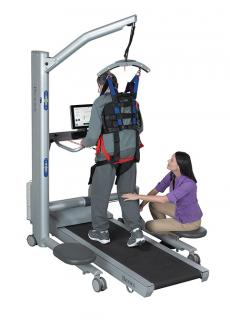
\includegraphics[height=3in]{gait_training.jpg} % first figure itself
%		\caption{Conventional gait rehabilitation. \cite{gaitrehabgantry}}\label{fig:gantry}
%	\end{subfigure}\hfill
%	\begin{subfigure}{0.45\textwidth}
%		\centering
%		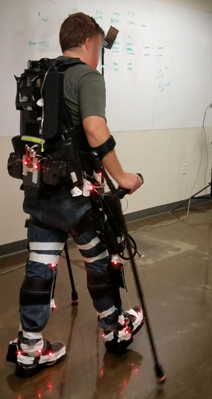
\includegraphics[height=3in]{subject.png}
%		\caption{EksoGT - powered exoskeleton}\label{fig:subject}
%	\end{subfigure}
%	\caption{Methods of gait rehabilitation}
%\end{figure}
%
%\begin{figure}
%	\centering
%	\begin{minipage}{0.45\textwidth}
%		\centering
%		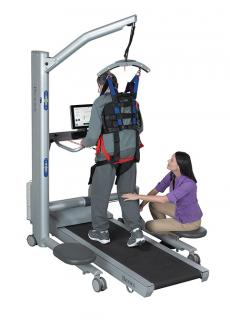
\includegraphics[height=3in]{gait_training.jpg} % first figure itself
%		\caption{Conventional gait rehabilitation. \cite{gaitrehabgantry}}\label{fig:gantry}
%	\end{minipage}\hfill
%	\begin{minipage}{0.45\textwidth}
%		\centering
%		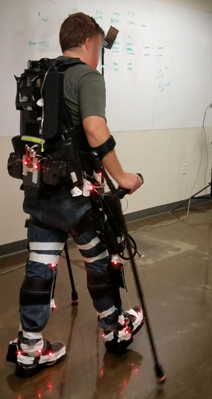
\includegraphics[height=3in]{subject.png}
%		\caption{EksoGT - powered exoskeleton}\label{fig:subject}
%	\end{minipage}
%\end{figure}
%
\begin{figure}
	\centering
	\subcaptionbox{Conventional gait rehabilitation. \cite{gaitrehabgantry}\label{fig:gantry}}[0.45\textwidth]{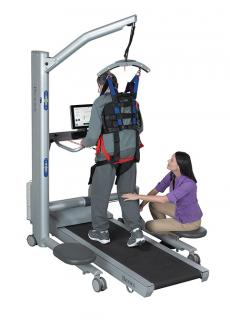
\includegraphics[height=3in]{gait_training.jpg}}%
	\hfill
	\subcaptionbox{EksoGT - powered exoskeleton \label{fig:subject}}[0.45\textwidth]{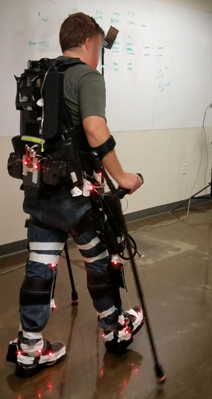
\includegraphics[height=3in]{subject.png}}%
	\caption{Methods of gait rehabilitation}
\end{figure}

\section{Motivation}
%
%\begin{figure}
%	\centering
%	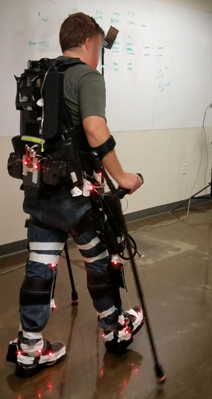
\includegraphics[width=0.15\linewidth]{subject.png}
%\end{figure}

Repeated walking practice has shown significant benefits in helping people with Spinal Cord Injury (SCI) achieve functional ambulation \cite{lam2007systematic}. The US has quarter-million existing cases of SCI with an additional 10,000 new cases annually \cite{nih} and the cost of care per patient with SCIs exceeds half a million dollars \cite{devivo2011costs}. Neural plasticity, the reorganization of the patient's intact neuronal pathways \cite{curt2008recovery}, is one of the main mechanisms of recovery from SCIs. To take advantage of this neural plasticity, gait rehabilitation strategies involve repeatedly moving the patient's legs through prescribed walking trajectories. Conventionally, this process involves physiotherapists manually moving the patient's legs to track the desired trajectories (Fig.~\ref{fig:gantry}). %The main drawback of this approach is that the necessary joint trajectories may not be tracked accurately as the treatment progresses due to therapist exhaustion. 
As this approach requires physical intervention from therapists, the lack of therapist appointments, or the need to administer therapy virtually may affect its feasibility. Robotic exoskeletons have come into use for rehabilitation due to their ability to consistently track the desired trajectories, which may accelerate recovery \cite{hidler2011role} with the therapist acting in a supervisory role.. Multiple exoskeletons, such as the Ekso GT \cite{brenner2016exploring} (Fig.~\ref{fig:subject}), Indego \cite{sup2008design}, and ReWalk \cite{rewalk}, have been cleared by the FDA for use in gait rehabilitation.

Exoskeleton usage increases the patient's level of autonomy and fluent Human-Robot Interaction (HRI) is desired to maintain the safety and efficacy of the treatment. While an abstract notion, fluency in HRI can be roughly defined as the reliability with which a human and robot can predict each other's actions~\cite{hoffman2007cost}. In addition to device safety, increasing fluency would help the user locomote more naturally and reduce the cognitive load on them caused by operating the device. Cognitive load affects gait patterns \cite{bogen2018walk} so reducing it may help exoskeleton users walk with more natural gaits. 

Fluency may be quantified by the inverse of the time it takes to complete desired tasks \cite{hoffman2019evaluating}. Fluency in HRI can be increased if the robot can anticipate the user's intent and assist accordingly. The overall goal of this work is to estimate user intent to increase the fluency of lower-extremity exoskeletons. Intent itself is difficult to quantify, so a user's desired forward velocity is considered as an expression of intent. Model-based and data-driven methods are considered to infer user intent by studying the effects of changes in velocity on gait patterns.

\section{Intent estimation for fluency in HRI}

A robot's ability to deliver timely assistance to the user is an important indicator of fluency. Anticipative intent estimation methods are necessary to reduce the delay in robot assistance delivery after the user has changed their intent as the timing of the assistance is crucial for fluent HRI. These methods estimate intent changes before they are physically realized, in contrast to reactive methods that detect changes after realization. Control actions necessary for assistance delivery may be decided in advance of when they need to be executed and assistance may be delivered more precisely due to anticipative intent inference. Intent is an abstract concept so it can be inferred in a variety of ways depending on how the estimation problem is posed.

\subsection{Model-based and learning-based approaches to estimation}
\begin{figure}
	\centering
	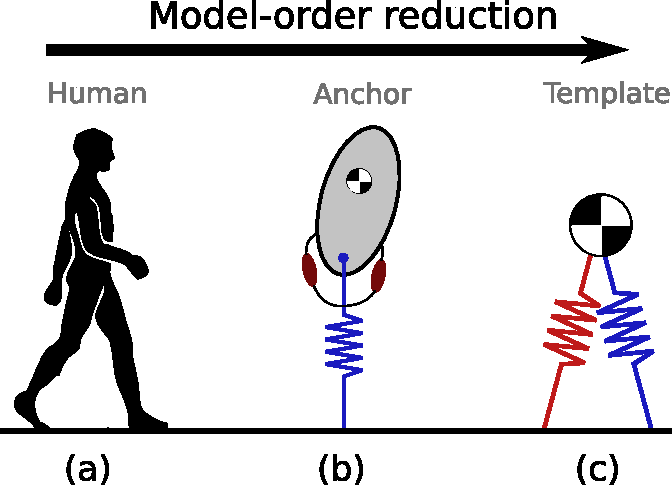
\includegraphics[width=0.55\linewidth]{abstraction.pdf}
	\caption{The model-order reduction of a human (a); (b) an anchor model, a neuromuscular model where the hip is actuated using Hill-type muscle models \cite{davoodi2019template}, (c) a template model, Bipedal Spring-Loaded Inverted Pendulum model \cite{geyer2006compliant}. }\label{fig:abstraction}
\end{figure}

Mechanically, humans are high degree of freedom systems but their gait patterns can often be accurately described by reduced-order models (Fig.~\ref{fig:abstraction}). Template models and anchor models~\cite{full1999templates} are reduced-order models used to describe human walking. Template models emulate the salient characteristics of locomotion and abstract the complexities of neuro-muscular interaction. Anchor models are higher fidelity models based on human morphology that combine template models with human physiology. The additional complexities found in anchor models make estimation and control based on these models more computationally intensive, rendering them inappropriate for use in online processes such as intent detection. While detailed musculo-skeletal models offer subject-specific insight into walking, the omission of these complexities in template models make them more suited for general use across subjects. This generality and reduced-order makes template models more suited for use in control and estimation problems for legged locomotion.

Template models often use parameters such as center of mass (CoM) height, velocity, and leg stiffness to describe gait \cite{geyer2006compliant,liu2015dynamic,full1999templates,sharbafi2015fmch}. It may be possible to estimate an exoskeleton user's intended forward velocity by comparing measurements of these parameters with gaits simulated using models of locomotion with the general scheme illustrated in Fig.~\ref{fig:schemes}. For example, intent estimation in lower-extremity exoskeletons based on orbital energy \cite{chen2018dynamic} has been carried out using the Linear Inverted Pendulum (LIP) model, which is a simple model of legged locomotion.  Alternatively, data-driven estimation strategies \cite{ge2011neural, kalinowska2019data, joukov2017rhythmic} may be used to handle gait characteristics that may be difficult to model using physics-based models.

\begin{figure}
	\centering
	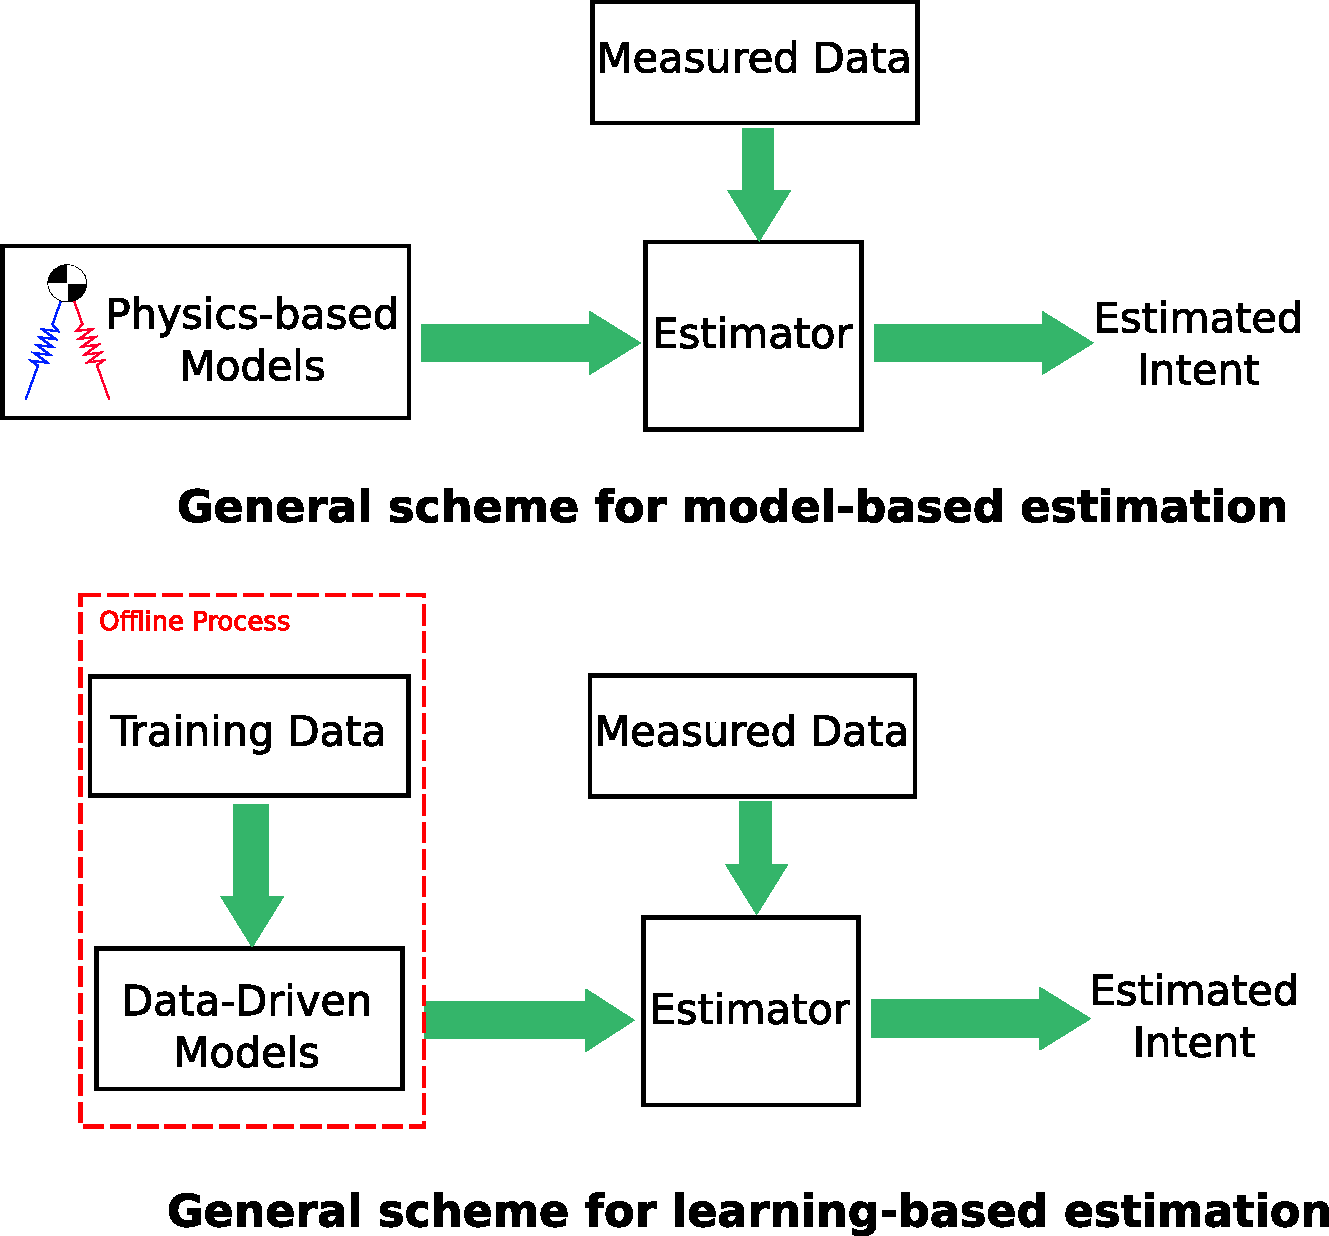
\includegraphics[width=0.6\linewidth]{schemes.pdf}
	\caption{General overview of model-based and learning-based estimation}\label{fig:schemes}
\end{figure}

Learning-based strategies use gait data to form relationships between sensor measurements and gait features such as foot placement and step frequency and these relationships may then be used for estimating user intent as illustrated in Fig~\ref{fig:schemes}. Convolutional Neural Networks (CNNs) \cite{lee2020image}, decision trees \cite{moolchandani2021design}, and Linear Discriminant Analysis (LDA) \cite{young2013classifying}  have all been used to estimate human intent in real-time with low error rates using sensors such as potentiometers and encoders onboard the prosthesis \cite{young2013classifying}, electrogoniometers \cite{lee2020image}, and force plates \cite{moolchandani2021design} in addition to  electromyography (EMG) and IMUs. A Gaussian Process (GP) based Extended Kalman Filter has been used to estimate a user's gait phase during stance to control a powered prosthetic leg \cite{thatte2019robust}.

\begin{figure}
	\centering
	\begin{overpic}[width=0.7\linewidth,percent]{intent_flow_chart.pdf}
		\put(14.5,23){\textcolor{NDgold}{\footnotesize \textbf{\cite{shen2013motion}}}}
		\put(28,3){\textcolor{NDgold}{\footnotesize \textbf{\cite{karulkarapplication,suzuki2007intention,brescianini2011ins}}}}
		\put(72,3){\textcolor{NDgold}{\footnotesize \textbf{\cite{Gambon20b,kalinowska2019data,thatte2019robust,sarac2013brain}}}}
	\end{overpic}
	\caption{Possible approaches to intent estimation. Approaches considered in this work have been indicated with green arrows.}\label{fig:flow}
	\vspace{-1em}
\end{figure} 

Different approaches to intent estimation as illustrated in Fig.~\ref{fig:flow}. One approach is to infer intent posed as a discrete variable and infer it by comparing measurements of user activity to a database of predefined activities such as sitting, standing, steady-state walking, and the transitions between them \cite{shen2013motion}. Generating databases containing a wide range of such activities may be prohibitive due to challenges involved in human subject trials. Alternatively, intent may be treated as a continuous state to achieve finer control of the assistive device. How someone interacts with a robot may be informative of their desired collaborative action.

\subsection{Leveraging Human-Robot Interaction for intent estimation}

Estimation of intent as a continuous variable may be performed by leveraging the HRI in gait rehabilitation. One study used physical Human Robot Interaction (pHRI) to estimate the user intent in collaborative reaching motions  \cite{corteville2007human}. In it, the human was considered to be in control of the HRI and measurements of the user's motion acquired using sensors onboard the robot were fit to a velocity profile to estimate the intended speed of the movement. 

Another approach to use pHRI for user intent estimation is to compare the user's efforts to the total effort necessary to accomplish the desired task \cite{pehlivan2015minimal}. Physical HRI is not limited only to interactions between the robot and the human. The human-robot system's interaction with the environment may also be considered pHRI and may be used to estimate user intent. For example, Inertial Measurement Units (IMUs) were mounted on crutches to estimate their orientation \cite{brescianini2011ins}. This configuration allowed the inference of user intent variables such as stride length, direction, and stair ascent/descent based on crutch placement. The reliance of many state-of-the-art approaches on sensors like EMGs, electrogoniometers, IMUs, force sensors may be problematic in practical applications as EMG sensors need consistency in placement and may slip during usage due to perspiration \cite{tkach2010study,ison2014role}. Therefore, relying on sensors onboard the exoskeleton may offer a more reliable option \cite{Gambon20b}. 

While pHRI may be used to infer an exoskeleton user's intent, the presence of injuries and their severity may limit the extent to which pHRI may be leveraged. HRI has been used to great effect in assisting healthy individuals walking in hip exoskeletons by modeling the impedance of the coupled human-robot system \cite{zhang2019admittance,nagarajan2016integral}. Hip torques generated by the user govern the assistance provided by the exoskeleton. However, it may be difficult to adapt these strategies to individuals with iSCIs due to significant lower-limb impairment. There are some available exoskeletons that are targeted toward individuals with iSCIs and they use rudimentary methods to infer user intent. The HAL exoskeleton uses force sensors under the feet to detect weight transfer to initiate a step \cite{suzuki2007intention} and the ReWalk system uses a combination of ground reaction force sensors and torso tilt \cite{goffer2012locomotion}. While these intent detection strategies leverage basic pHRI, using additional gait variables to obtain information for intent estimation may provide additional insight into the user's desired motion. An exoskeleton's gait patterns may be analyzed to infer their intent using model- or learning-based strategies, proceeding to the third level of Fig.~\ref{fig:flow}. This work is targeted toward individuals with iSCIs whose gait patterns depend on the severity of the injury \cite{rota2011walk}. Therefore, subjects' interactions with the robot and the environment may show individualized trends making estimator personalization necessary for intent change estimation from gait patterns. 

\subsection{Personalizing intent estimation and addressing data scarcity}

Learning-based approaches for intent estimation often rely on large amounts of data to generate models of gait features\cite{lee2020image,moolchandani2021design}. Acquiring this data for an injured population is made increasingly difficult due to changes in gait patterns resulting from the severity of injuries \cite{sohn2018variability}. The difference in gait patterns across individuals makes the need for estimator personalization unavoidable. Acquiring adequate amounts of data to train a single model to perform estimation across multiple individuals is difficult as gait variability resulting from spasticity due to iSCIs \cite{krawetz1996gait} needs to be accommodated. Data scarcity may be addressed by pooling training data from multiple subjects.

There is underlying commonality, across individuals, in changes to gait patterns relating to changes in gait velocity \cite{li1999coordination}. For example, step length and frequency, pitch and roll motions of the torso, and joint trajectories all show qualitatively similar trends relating to changes in the desired gait velocity across individuals. Training data scarcity may be addressed by exploiting this commonality to personalize intent estimation by transforming easily accessible gait data from healthy individuals using a small amount of appropriately selected user-specific data.

\section{Contributions and organization}

Multiple robotic exoskeletons have been approved by the FDA for gait rehabilitation of individuals with iSCIs, yet the intent change estimation in these devices is reactive and limited to detecting when the user wants to initiate a new step of a predefined gait pattern. This limitation also prevents sudden velocity changes. As a result, these devices are generally seen in clinical settings and their operation requires physiotherapist supervision. Anticipative user intent estimation in these devices may take these devices closer to being used unsupervised, which may lead to increased usage and accelerated rehabilitation \cite{hidler2011role}. This dissertation makes contributions with an aim to advance the state-of-the art of intent estimation to be more anticipative of changes in the user's intent as expressed through gait speed.

Chapter~\ref{chapter:bg_info} focuses on background information that forms the foundation of the contributions presented herein. This chapter discusses the basics of modeling human locomotion and gait periodicity using Poincar\'e maps. Additionally the chapter also explains the concept of state estimation with Kalman filter and describes two variations of the filter. Details of the exoskeleton trial data used to evaluate the estimators presented herein are also included in this chapter.

Accurate state estimation is a foundational component for intuitive user intent detection in HRI, as it would deliver increased insight into user actions. Chapter~\ref{chapter:IMM} details first contribution; to study the gait patterns seen during slow walking and establish a framework capable of handling hybrid dynamics seen in models of legged locomotion. This framework was then used to estimate gait characteristics such as gait phase, by comparing simulated gaits of physics-based models of legged locomotion to measurements taken during walking trials with the exoskeleton. 

The work presented in Chapter~\ref{chapter:BKF} uses the insights about walking in an exoskeleton gained from the previous chapter to develop an estimator that anticipates changes in the exoskeleton user’s intended gait velocity. In contrast to many state-of-the-art intent estimators that are reactive, the presented framework anticipatively estimates a user's desired gait speed by analyzing how the user interacts with the robot and the environment to realize the desired change. This estimator was evaluated with walking trial data of	individuals with and without iSCIs walking in an EksoGT exoskeleton and the differences in the HRI of injured and uninjured users were also explored.

Chapter~\ref{chapter:MP} builds on the estimator framework presented in Chapter~\ref{chapter:BKF}. The inter-subject gait variability observed across exoskeleton users motivated estimator personalization for anticipating speed changes. One of the main hurdles in achieving the required personalization is the scarcity of user-specific training data due to difficulty in acquisition. Estimator personalization was achieved by exploiting commonalities in gait patterns across users and augmenting data from healthy subjects with user-specific data from subjects with iSCIs. Additionally, the work presented in this chapter also describes methods to discover user-specific relevance of gait features to gait speed and ensure estimator quality while personalizing gait speed estimation.

Chapter~\ref{chapter:conc} provides concluding remarks and introduces topics for future work that have emerged from the work presented in this dissertation.

%\begin{itemize}
%	%\item \textbf{Contribution 1: Model-based Approach to Estimate Gait Characteristics:} 
%	\item Accurate state estimation is a foundational component for intuitive user intent detection in HRI, as it would deliver increased insight into user actions. The first contribution was to establish a framework capable of handling hybrid dynamics to estimate gait characteristics such as gait phase, using simulated gaits of physics-based models of legged locomotion (Chapter~\ref{chapter:IMM}).
%	%\item \textbf{Contribution 2: Intent Change Estimation Based on Physical Interactions of an Exoskeleton User:} 
%	\item In contrast to many state-of-the-art intent estimators that are reactive, this objective is to develop an estimator that anticipates changes in the exoskeleton user’s intended gait velocity by analyzing how the user interacts with the robot and the environment to realize the desired change. This estimator was evaluated with walking trial data of	individuals with and without iSCIs walking in an EksoGT exoskeleton. The differences in the interactions of injured and uninjured users was explored (Chapter~\ref{chapter:BKF}).
%	%\item \textbf{Contribution 3: Personalization of Estimation in the Presence of Data Scarcity:}
%	\item The inter-subject gait variability observed across individuals motivated personalizing estimation of changes in intended gait velocity of exoskeleton users. One of the main hurdles in achieving the required personalization is the scarcity of user-specific training data due to difficulty in acquisition. Estimator personalization was achieved by exploiting commonalities in gait patterns across users and augmenting base data from healthy subjects with user-specific data from subjects with injuries (Chapter~\ref{chapter:MP}).
%\end{itemize}
	%
	% Background Information
	\chapter{Background Information}

The work presented herein draws on multiple concepts to model human walking and estimate intent. This chapter serves to provide background information to familiarize the reader with the fundamentals of these concepts before elaborating on the goals of the dissertation in subsequent chapters. Every estimation scheme depends on a model of the underlying process, the same is true for gait velocity estimation.

\section{Models of legged locomotion}

Modeling gait walking is one of the main components of gait velocity estimation and it may be achieved using simple physics-based template models. Physics-based models may be actuated or passive i.e., without any control inputs.  

\subsection{Actuated Models}

One approach to gait modeling is including a control input to achieve the desired gait. An example of this approach is the Variable-SLIP (V-SLIP) model, which utilizes variable stiffness actuation to modulate leg stiffness in contrast to the original B-SLIP model that has constant leg stiffness~\cite{visser2017bipedal}. This model produces a gait that is robust to disturbances, and whose cost of transport is comparable to human walking\footnote{Cost of transport quantifies the energy efficiency of a system, it measures the energy expended to travel a specified distance.}. Another approach is to vary the CoM height by applying a force along the leg~\cite{koolen2016balance}. While all the previously described models have nonlinear dynamics, Kajita et al.~\cite{kajita1991study} proposed a model called the Linear Inverted Pendulum (LIP) model in which the application of a constraint control input linearizes the dynamics of the system. The LIP model also allows the use of ankle torques to improve model performance on rugged terrain. The LIP model has been extended to three dimensions with the 3D-LIP model~\cite{kajita20013d}.

Actuated models provide a more flexible framework to estimate gait, but determining the control parameters when applying those models to humans becomes a challenge. Therefore, active models are more suited to legged robots or prosthetic devices which are used in series with the user. The simplicity of passive models and the ability to modify the initial conditions to accommodate the effects of a user working in parallel makes them more suited for parallel robots such as exoskeletons. Most active models have been proposed in regards to legged robots where the dynamics of the robot are well known to the designers. This allows for the complexity of the model to be matched to the complexity of the system dynamics. With the case of exoskeletons, the dynamics of the human body are still a subject of study and they are further complicated by the parallel operation with the exoskeleton suit due to coupling in the human and robot. As a result, passive models may be better suited for use in intent detection frameworks due to their relative simplicity.

\subsection{Passive Models}

It has been shown that passive models can accurately generate gaits that qualitatively resemble key features of human locomotion~\cite{mochon1980ballistic}. The most basic passive model is an inverted pendulum (IP) with the center of mass (CoM) vaulting over a stiff leg. However, it was observed that animal gaits exhibit significant energy storage in muscles, tendons, and ligaments. As a result, legged locomotion may be analogous to a spring-mass system~\cite{blickhan1989spring} with the CoM loaded onto a compliant leg, modeled as a spring. This characterization of legged locomotion could not be reconciled with the stiff leg utilized in the IP model and a new model, called the Spring-Loaded Inverted Pendulum (SLIP), was proposed to add compliance to the leg via a massless spring~\cite{blickhan1989spring}. It has been observed that relative leg stiffness of animals ranging from dogs and rams to humans and kangaroos is similar during running~\cite{blickhan1993similarity} and that the CoM falls to its lowest position at midstance across species, compressing a virtual spring and releasing that stored energy as the gait progresses~\cite{full1999templates}. This dynamic similarity can be further reinforced using the Froude numbers for various animals. The Froude number is a metric that non-dimensionalizes velocity with leg length and gravity. Multi-legged animals exhibit gait transitions at similar Froude numbers, suggesting that may be possible to use template models to capture gaits for a more generalized set of subjects with respect to their morphology.

The SLIP model can be used to describe human running, however, it is inadequate to describe human walking. The IP model exhibited CoM trajectories with higher vertical oscillation than observed in human trials for both walking and running~\cite{lee1998determinants}. The discrepancy in the CoM trajectories was found to increase with forward velocity. The IP and SLIP models lack the double support phase, which is crucial during walking. These deficiencies were addressed when Geyer proposed an extension of the SLIP model, called the Bipedal-SLIP (B-SLIP) model, in which the CoM is supported by two massless springs of fixed stiffness~\cite{geyer2006compliant}. The  B-SLIP model matches human CoM trajectories and ground reaction force (GRF) profiles, at average walking and running velocities. Thus the B-SLIP model is a unified model that can exhibit multiple gaits across a range of velocities. While the B-SLIP model addresses the shortcomings of IP and SLIP models, it has its drawbacks when walking at extreme velocities. The model exhibits oscillations during the double support phase at low velocities in the range of walking speeds exhibited by individuals with SCIs. These oscillations may be the result of the 2D nature of these models.

In their basic forms, the IP, SLIP and B-SLIP models all ignore lateral dynamics, however, lateral dynamics become more dominant for low-speed gaits. For example, according to the human walking data presented by Fukuchi et al.~\cite{fukuchi2018public}, the peak-to-peak amplitude of the lateral sway of the CoM is approximately 3 cm while walking at 1.27 m/s but it rises to 9 cm while walking at 0.44 m/s. The model presented by Geyer is defined in only two dimensions, but it generalizes to 3D~\cite{liu2015dynamic}. This 3D model allows the lateral sway to be taken into consideration and oscillations during double support are eliminated. With appropriate leg length and step width, the sway seen in the gaits generated using the 3D B-SLIP model is comparable to human data. Taking the lateral sway into consideration is especially important while studying walking at low speeds. 

\section{The B-SLIP model}
The work presented herein is focused on individuals recovering from iSCIs whose walking velocities were as low as 0.4 m/s. A majority of the the duration of steps at low velocities is spent in double support, and it is important to use a model than can describe this gait phase. Therefore, this work considers the 3D B-SLIP model to model human locomotion shown in Fig~\ref{fig:slip}. In this model, the \COM~is loaded onto two massless spring legs of length $ l_o $ and stiffness $ k $. The position and velocity of the point mass $ m $ are given by $ \p_{\COM} = [x_{\COM} ,y_{\COM} ,z_{\COM}]^T $ and $ \v_{\COM} = [v_x ,v_y ,v_z]^T $. The position of the leading leg at touchdown is given by two angles, the angle between the leading leg and vertical $ \theta $ and the angle $ \varphi $ between the forward axis $ x $  and the ground projection of the leading leg.
%
\begin{figure}
	\centering
	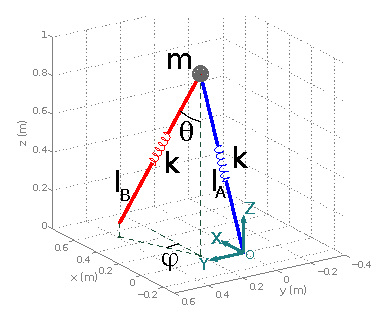
\includegraphics[width=0.6\linewidth]{3DSLIP.eps}
	\caption{The Bipedal Spring Loaded Inverted Pendulum \cite{liu2015dynamic} model of walking}\label{fig:slip}
\end{figure}
%
\begin{figure}
	\centering
	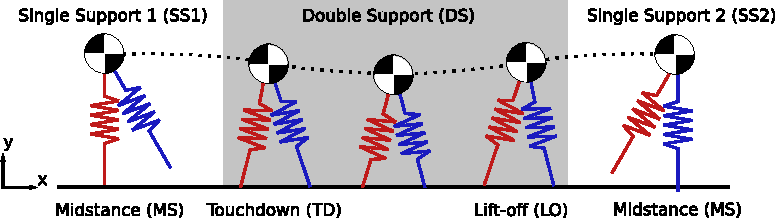
\includegraphics[width=\linewidth]{slip_gait.pdf}
	\caption{One step of a B-SLIP gait}\label{fig:slip_gait}
\end{figure} 
%

A gait of the B-SLIP model, as viewed in the sagittal plane \footnote{The saggital plane is the plane that divides the body into right and left parts.}, is illustrated in Fig.~\ref{fig:slip_gait}. This gait starts at midstance (MS), where the CoM is loaded onto the trailing leg in single-support (SS1). The gait then proceeds with the touchdown (TD) of the leading leg and enters the double support (DS) phase. The DS phase ends with lift-off (LO) of the trailing leg and the model enters the second single-support phase (SS2). The SS2 phase ends in MS, again with the CoM loaded onto the leading leg. As there are alternating SS and DS phases, the dynamics of the B-SLIP model are hybrid.

\subsection{Hybrid dynamics of the B-SLIP model}
The dynamics of the model in single support are described by
\begin{equation}
	m\ddot{\p_{\COM}} = k(l_0 - \lVert \mathbf{l}_i \rVert)\hat{\mathbf{l}}_i + m \mathbf{g}
\end{equation}
\noindent where $ i = \{A,B\} $ denotes the supporting leg, $ \mathbf{l}_i \in \mathbb{R}^3 $ is the vector along the leg from the mass to the position of the stance foot $\p_i$ , $ \hat{\mathbf{l}}_i \in \mathbb{R}^3$ is a unit vector along the leg, and $ \mathbf{g} \in \mathbb{R}^3 $ is the gravity vector. The dynamics during double support are given by
\begin{equation}
	m\ddot{\p_{\COM}} = k(l_0 - \lVert \mathbf{l}_A \rVert)\hat{\mathbf{l}}_A + k(l_0 - \lVert \mathbf{l}_B \rVert)\hat{\mathbf{l}}_B + m \mathbf{g}
\end{equation}
%
\noindent Certain conditions, known as guards, must be met to enable the switching of the dynamics from one phase to another. There are three switching surfaces to enable phase switches at TD, LO, and MS. These sets are as follows
%
\begin{eqnarray}
	\mathcal{G}_{TD} &=& \{(\p,\v)| v_z < 0 ,z_{\COM} < z_{T}\} \\
	\mathcal{G}_{LO} &=& \{(\p,\v)| v_z > 0 ,\lVert \mathbf{l}_A \rVert > l_0\} \\
	\mathcal{G}_{MS} &=& \{(\p,\v)| v_z = 0 ,z_{\COM} > z_{T} ,\lVert \mathbf{l}_A \rVert < l_0\} 
\end{eqnarray} 
%
\noindent where $ z_{T} = l_0 \cos \theta $ is the threshold height for touchdown. Satisfaction of these guard conditions triggers gait phase switches and the states of the model are transferred across the switching events using functions called reset maps. There are three reset maps for the B-SLIP model following the general form $ \x^+ = \mathcal{R(\x^-)} $, where the $ + $ and $ - $ denote pre- and post-switch states. One map is applied at TD and the other at LO such that
%
\begin{eqnarray}
	\mathcal{R}_{TD}:\x^- &\rightarrowtail& I\x^- :\mathbb{R}^6 \rightarrowtail \mathbb{R}^6 \\
	\mathcal{R}_{LO}:\x^- &\rightarrowtail& I\x^- ,\p_B \leftarrow \p_A :\mathbb{R}^6 \rightarrowtail \mathbb{R}^6 \\
	\mathcal{R}_{MS}:\x^- &\rightarrowtail& I\x^- :\mathbb{R}^6 \rightarrowtail \mathbb{R}^6
\end{eqnarray}
%
The are not impacts at touchdown as spring legs of the B-SLIP model are assumed to be massless. Reset maps handle touchdown impacts for models that consider the mass of the feet. Thus, the B-SLIP model can exhibit periodic gaits by alternately switching through SS and DS phases.

As the B-SLIP model is passive, it does not have any active control inputs to modify gaits and maintain periodicity. Therefore, optimization methods need to be used to find periodic model gaits as steady-state human walking is periodic. Poincar\'e maps are used in the gait optimization \cite{strogatz2018nonlinear,garcia1998simplest} to find periodic gaits.

\section{Poincar\'e maps}

\begin{figure}
	\centering
	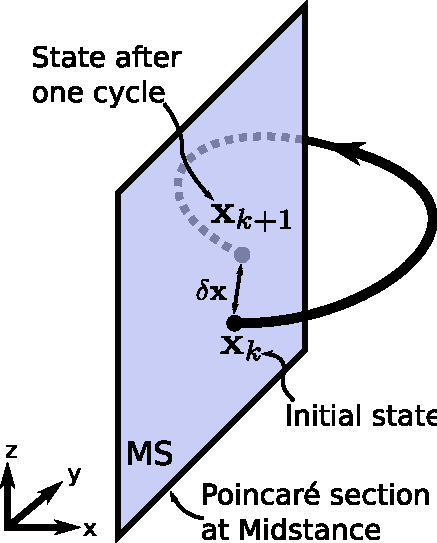
\includegraphics[width=.3\linewidth]{poincare.pdf}
	\caption{A Poincar\'e map used to find periodic gaits}\label{fig:poincare}
\end{figure}

A Poincar\'e section for a dynamical is a subspace that has fewer dimensions that the model's state space. It may be placed at a gait event such as MS, TD, or LO when the value of one of the states may be known i.e., when a guard condition is met. Let the Poincar\'e section be placed at MS, and let $ \mathcal{P}(\x_k) $ be a function that returns the state after one cycle, or a step in the case of the B-SLIP, such that $ \x_{k+1} = \mathcal{P}(\x_k) $. Then function $ \mathcal{P}(\x_k) $ is the Poincar\'e map and there exists an initial state called a fixed point, representing a periodic orbit where the initial state maps back to itself after one period such that $ \x_k = \mathcal{P}(\x_k) $.
%
%\begin{equation}
%	\x_k = \mathcal{P}(\x_k)
%\end{equation}
%

A Poincar\'e section placed at MS is shown in blue in Fig.~\ref{fig:poincare}. The dynamics of the model are integrated for one step using $ \x_k $ as the initial condition. Optimization methods are used to find initial conditions that yield periodic gait by minimizing $ \delta \x $, the error between $ \x_k $ and $ \x_{k+1} $. The nonlinear return map may be linearized about these periodic gaits for further refining the gait search as described in Chapter~\ref{chapter:IMM}. Model gaits for various velocities may be used as references while estimating an exoskeleton user's desired gait. Measurements of quantities such as \COM~height and velocity, may be compared to simulated model gaits using state estimation tools such as the Kalman filter. 

\section{State estimation using Kalman filters}

Kalman filtering is a feedback-based sequential optimal estimation technique \cite{kalman1960new} to estimate states and parameters of dynamical systems. The estimates made by the filter are conditioned on certain measurements of either the states themselves or other quantities that may be represented as a functions of the states through a measurement model. State estimation is reliant on these measurements to get a picture of the real world, however these measurements rarely free of noise that may adversely affect the quality of the state estimates. 

Kalman filters follow a predictor-corrector scheme in which states are propagated using a model of system dynamics which may be incomplete. These states are then corrected using the residual between sensor measurements and the predictions. If the feedback gain applied to this residual is too low, state estimates will not be appropriately corrected, and if the gain is too high, the noise model will overshadow the system dynamics and the estimates will begin tracking noise. Kalman filtering presents an optimal method of computing feedback gain that accounts for modeling and measurement errors with a fundamental assumption that any modeling or measurement errors are zero-mean Gaussian noise processes. The filter was originally proposed for discrete-time linear systems. 
 
\subsection{Discrete-time Kalman Filter}
The filter is initialized at a certain initial state estimate $ \hat{\x}_0 $ that may have associated uncertainty due to measurement errors. The evolution of this state is described using dynamical system presented in the following equations
%
\begin{eqnarray}
	\x_{k+1} &=& \A_k \x_k + \B_k \u_k + \mathbf{G} \mathbf{w}_k,\quad \mathbf{w}_k \sim \mathcal{N}(0, \Q_k) \label{eq:sys_disc}  \\
	\tilde{\y}_k &=& \H_k \x_k + \mathbf{v}_k,\quad \mathbf{v}_k \sim \mathcal{N}(0,\R_k) \label{eq:meas_lin}
\end{eqnarray}
%
\noindent where $ \x_k $ and $ \u_k $ are the discrete-time states and inputs, $ \y_k $ are the discrete-time measurements, $ \A_k $, $ \B_k $, $ \H_k $ are the system, input, and measurement models respectively. The system has zero-mean Gaussian noises for process noise $ \mathbf{w}_k $ and measurement noise $ \mathbf{v}_k $ with covariances  $ \Q_k $ and $ \R_k $ respectively. The measurement noise $ \mathbf{w}(t) $ is combined with the measurement equation $ \H_k \x_k$ to form the noisy measurement $ \tilde{\y}_k $. 
%
\begin{figure}
	\centering
	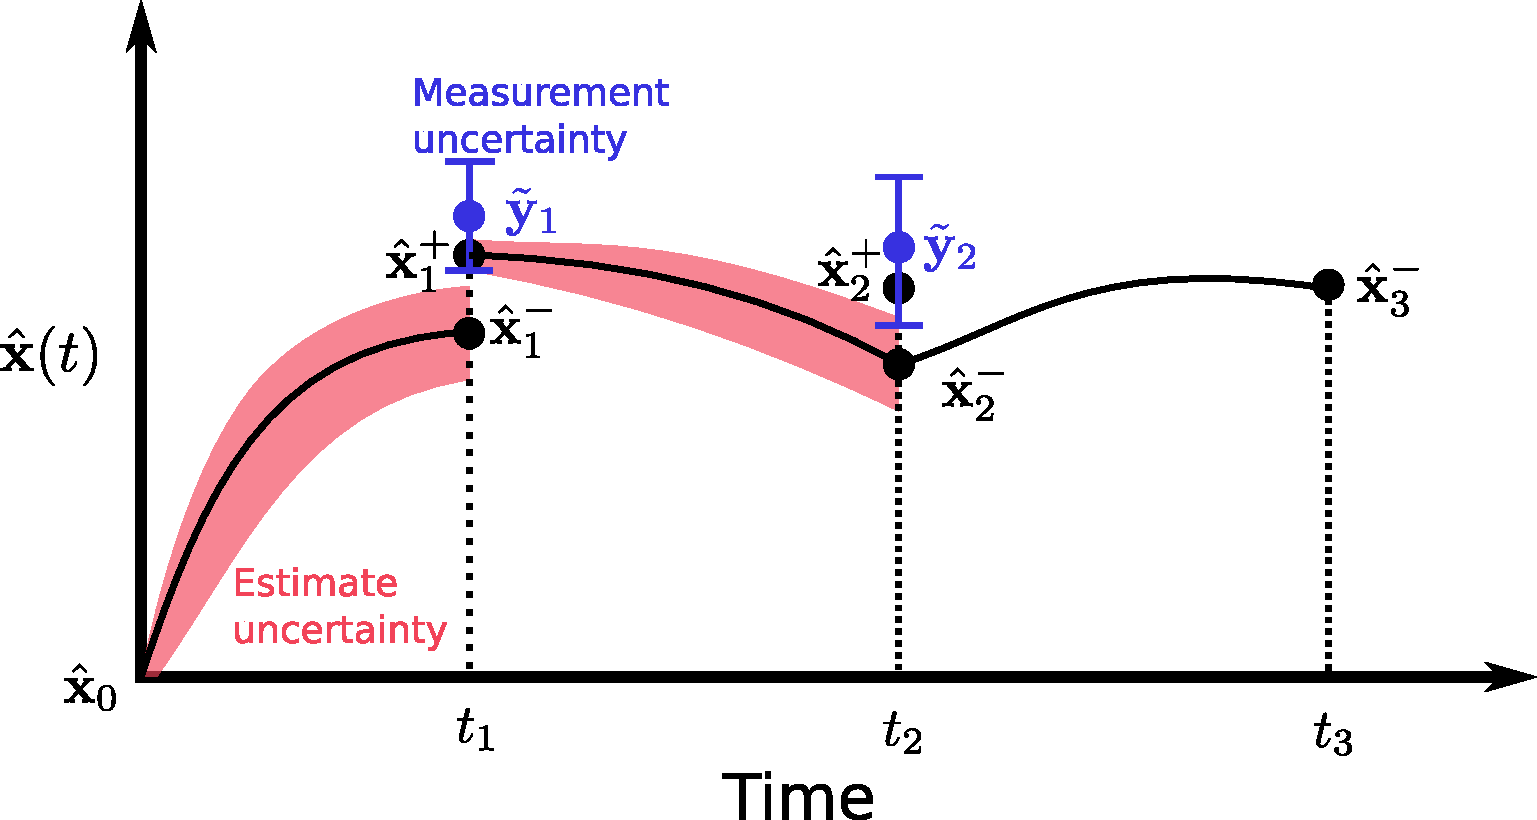
\includegraphics[width=0.8\linewidth]{kalman.pdf}
	\caption{Illustration of the Kalman Filtering process}\label{fig:kalman}
\end{figure}
%
The uncertainty associated with the estimates increases as the state is propagated forward through time using the system dynamics. Regular measurements of state variables are used to update the state estimates and reduce the uncertainty as illustrated in Fig.~\ref{fig:kalman} where the $ + $ and $ - $ in the superscript denote pre- and post-update states. The system illustrated here is discrete, however a continuous state evolution is shown to better illustrate the growth in uncertainty. Kalman filters account for both, the uncertainty in the state estimates and in the measurements. Further details of this process are as follow. The state estimates and estimate covariance $ \P $ are propagated in discrete time such that
\begin{eqnarray}
	\hat{\x}_{k+1} &=& \A_k \hat{\x}_k + \B_k \u_k \\
	\P_{k+1} &=& \A_k\P_k \A_k^T + \mathbf{G}_k\Q_k\mathbf{G}_k^T 
\end{eqnarray}
\noindent The states are sequentially updated such that
\begin{eqnarray}
	\K_k &=& \P_k^- \H^T_k \left[\H_k \P_k^- \H^T_k + \R_k\right]^{-1} \\
	\hat{\x}_k^+ &=& \hat{\x}_k^- + \K_k[\tilde{\y}_k- \H_k \hat{\x}_k^-)] \\
	\P_k^+ &=& [\mathbf{I} - \K_k \H_k]\P_k^-
\end{eqnarray}
%
\noindent where the updated estimates, their covariance and the Kalman gain are $ \mathbf{x}_k^+ $, $ \mathbf{P}_k^+ $, and $ \K_k $ respectively. The Kalman gain is optimal and the error dynamics of the filter are shown to be stable \cite{Crassidis} using the Lyapunov candidate function $ V(\e) = \e_k^T P_k^{-1} \e_k $ where $ \e_k \equiv \hat{\x}_k - \x_k $. The filter as described above is defined for linear systems, and it has been extended to nonlinear systems.

\subsection{Extended Kalman Filter}
Simple models used to describe legged locomotion have nonlinear dynamics and a variation of the Kalman filter named the Extended Kalman Filter (EKF) can be used for these systems. The nonlinear dynamics are linearized about the state estimate to work around the nonlinearity. As this linearization is an approximation of the dynamics, the EKF is not optimal like the discrete-time Kalman filter described previously. In spite of the lack of optimality, EKFs have been in widespread use for nonlinear systems. Since most nonlinear dynamics are given in continuous time, a variation of the EKF called the Continuous-Discrete EKF may be used. In this variation, dynamics evolve in continuous time, and measurements are modeled in discrete time. This combination is used for estimation in the work presented herein as it most closely reflects the model and measurement conditions observed in the estimation problem being studied. The general structure of the EKF is similar to the filter presented previously, except the equations are nonlinear as seen by comparing Eq. \eqref{eq:sys_disc} and \eqref{eq:sys}. Consider the following dynamical system with nonlinear dynamics
% Continuous-Discrete EKF
%
\begin{eqnarray}
	\dot{\x}(t) &=& \mathbf{f}(\x(t),\u(t),\mathbf{w}(t),t),\quad \mathbf{w}(t) \sim \mathcal{N}(0, \Q(t))  \label{eq:sys}  \\
	\tilde{\y}_k &=& \mathbf{h}(\x_k) + \mathbf{v}_k,\quad \mathbf{v}_k \sim \mathcal{N}(0,\R_k) \label{eq:meas}
\end{eqnarray}
%
\noindent where $ \x(t) $ and $ \u(t) $ are the continuous-time states and inputs, $ \y_k $ are the discrete-time measurements, and $ \mathbf{f}(\x(t),\u(t),t) $ and $ \mathbf{h}(\x_k) $ are the system and measurement function respectively. The system has zero-mean Gaussian process and measurement noises $ \mathbf{w}(t) $ and $ \mathbf{v}_k $ respectively with covariances $ \Q(t) $ and $ \R_k $ respectively. The measurement noise $ \mathbf{w}(t) $ is combined with the measurement equation $ \mathbf{h}(\x_k) $ to form the noisy measurement $ \tilde{\y}_k $. 

The state estimates and estimate covariance $ \P $ are propagated in continuous time such that
\begin{eqnarray}
	\dot{\hat{\x}} &=& \mathbf{f}(\hat{\x},\u,t) \\
	\dot{\P}(t) &=& \F(t)\P(t) + \P(t)\F^T(t) + \mathbf{G}(t)\Q(t)\mathbf{G}(t)^T \\ 
	\F(t) &\equiv& \frac{\partial \mathbf{f}}{\partial \x} \Bigr |_{\hat{\x}(t),\u(t)} \nonumber
\end{eqnarray}
%
\noindent The states are sequentially updated such that
\begin{eqnarray}
	\K_k &=& \P_k^- \H^T_k(\hat{\x}_k^-) \left[\H_k(\hat{\x}_k^-)\P_k^- \H^T_k(\hat{\x}_k^-) + \R_k\right]^{-1} \\
	\hat{\x}_k^+ &=& \hat{\x}_k^- + \K_k[\tilde{\y}_k-\mathbf{h}(\x_k)] \\
	\P_k^+ &=& [\mathbf{I} - \K_k \H_k(\hat{\x}_k^-)]\P_k^-,\quad \H_k(\hat{\x}_k^-) \equiv \frac{\partial \mathbf{h}}{\partial \x} \Bigr |_{\hat{\x}_k^-}
\end{eqnarray}
%
\noindent where $ \K_k $ is the Kalman gain, $ \F(t) $, and $ \H_k(\hat{\x}_k^-) $ are the linearized dynamics and measurement model respectively. The updated estimates and their covariance are $ \mathbf{x}_k^+ $ and $ \mathbf{P}_k^+ $ respectively. The above equations describe a Continous-Discrete Kalman filter setup. System dynamics are propagated in continuous time but states are updated in discrete time since measurements are discrete. This setup handles the nonlinear dynamics of the models used to emulate legged locomotion. Each step of human walking has alternating single and double support periods depending on how many legs are in contact with the ground. Therefore, addition to being nonlinear, models of legged locomotion have hybrid dynamics to describe different gait phases i.e., different dynamics for different phases. The EKF can be used as an estimation tool to handle these hybrid dynamics in a framework known as Interacting Multi-Model (IMM) estimation. This framework is used in Chapter~\ref{chapter:IMM} to estimate an exoskeleton user's gait speed and gait phase.
	%
	% IMM
	\chapter{Model-based Approach to Estimate Gait Characteristics} \label{chapter:IMM}
The target population of this work is individuals with iSCIs, so the gait velocities of interest are very small in magnitude ($ \sim $ 0.5 m/s) \cite{nymark2005electromyographic}. There is limited work that uses physics-based models as a fundamental component in intent detection. The main attraction of using physics-based models is to allow for the accommodation of a greater number of users by modifying a small set of parameters such as mass, leg length, angles, and stiffness. This contribution uses the 3D B-SLIP model \cite{liu2015dynamic} as the basis of an estimation framework.

There are often physical changes to the gait as a result of changes in intended velocity, such as changes in step frequency, step length, and CoM trajectories \cite{kuo2001simple}. Template models emulate the salient characteristics of legged locomotion such as CoM trajectories and ground reaction force (GRF) profiles \cite{mochon1980ballistic}. Therefore, they may also emulate the changes in CoM trajectories and step length corresponding to changes in intent. The purpose of this contribution is to estimate gait characteristics such as gait phase and velocity through the comparison of sensor measurements to gaits from models of bipedal locomotion, specifically the B-SLIP model. The main idea behind the estimation framework developed is to estimate a person's desired gait velocity and phase by comparing the measured CoM trajectory to those in a library of B-SLIP gaits. 

User intent estimation may not necessarily be limited to forward velocity. Other aspects of intent changes not considered herein are the user's desires to initiate/terminate gait, change heading, and change gait mode i.e., transitions from walking on flat ground to ramps or stairs. In theory, the presented IMM framework may be extended to all these scenarios, with appropriate models of locomotion e.g., the B-SLIP model cannot describe gait initiation/termination. Considering multiple aspects of intent change for estimation at once may present difficulties as they may influence the gait differently and complicate the estimation problem via crosstalk. Considering only the gait velocity as a starting point helps break the estimation problem into a smaller subsection and reduces the challenges faced during estimation.

The challenges faced during estimation were the increased difficulty in finding low-speed periodic gaits during gait library generation and handling the hybrid dynamics of legged locomotion used to describe the different gait phases. The work done to address these challenges is described in this chapter. A linearization-based seed search method was developed to search for gaits at low walking speeds (less than 0.8 m/s). Additionally, Interacting Multi-Model (IMM) estimation was used to handle hybrid dynamics along with the library gaits. This chapter describes the results reported in a previous conference publication \cite{karulkarapplication}.

\section{Generating the gait library using the B-SLIP model}

Qualitative differences in the CoM trajectories of humans walking at different were observed in experimental data. Namely, the vertical and lateral excursion of the CoM over each step increase as gait velocity decreases. It was hypothesized that gait parameters may be estimated based on the changes in CoM trajectories. The 3D B-SLIP model presents a balance between model simplicity and CoM trajectory emulation. Additionally, using the 3D B-SLIP model allows the modeling of two important attributes of walking at low speeds; the lateral CoM movement that becomes increasingly dominant as gait velocity decreases and the DS period that represents a majority of the gait cycle. As the B-SLIP is a passive model, the omission of an actuator simplifies the estimation problem by reducing the assumptions necessary while applying these models to human walking. 

As described in Section~\ref{sec:bslip_model}, the state vector representing the CoM is $ \x_{CoM} = \left[x_{CoM} ,y_{CoM} ,z_{CoM} ,\dot{x}_{CoM} ,\dot{y}_{CoM} ,\dot{z}_{CoM}\right]^T $. The remaining parameters of the model, leg angles and stiffness, are collected in a parameter vector $ \greekvec{\zeta} = [\phi, \theta ,k ,z_{0_{CoM}} ,y_{0_{CoM}} ,\dot{x}_{0_{CoM}}]^T $ where $ \theta $ and $ \phi $ are leg angles that govern step length and width, and variables $ z_{0_{CoM}}$, $y_{0_{CoM}}$, and $\dot{x}_{0_{CoM}} $ give the vertical position, lateral position, and forward velocity of the CoM relative to the stance foot at the beginning of the step. The lack of actuators means optimization methods must be used to find periodic gaits for the B-SLIP model. An optimization procedure was carried out to find the parameters that would yield a fixed point for an MS-to-MS Poincar\'e map.

\subsection{Gait Optimization}
%
\begin{table}
	\centering
	\caption{Components of the gait optimization cost function \label{table:cost}}
	\small
\begin{tabular}{|c|m{0.7\linewidth}|}
	\hline
Cost component	& \multicolumn{1}{c|}{Description} \\
	\hline
$ z_{0_{CoM}} - z_{MDS} $	& Residual between CoM height at MS and Mid-Double-Support (MDS) to minimize vertical excursion. \\
	\hline
$ y_{0_{CoM}} - y_{foot_A} $	& Minimize distance of CoM ground projection to foot at MS. \\
	\hline
$ l_{step_{des}} - l_{step} $	& Residual between desired and actual step length. \\
	\hline
$ w_{step_{des}} - w_{step} $	& Residual between desired and actual step width. \\
	\hline
\end{tabular}




%\begin{eqnarray}
%	l_{step_{des}} &-& l_{step} \\
%	w_{step_{des}} &-& w_{step} \\
%	z_{0_{CoM}} &-& z_{MDS} \\
%	y_{0_{CoM}} &-& y_{foot_A}
%\end{eqnarray}
%
%$ g(\xi) $ are nonlinear constraints that ensure periodicity of the gait. 

\end{table}
%

Gait optimization was considered via a nonlinear programming problem
%
\begin{eqnarray}
	\min_{\greekvec{\xi}}& \quad \lVert{\mat{J}(\greekvec{\xi})}\rVert ^2 + (k_{max} - k) \label{eq:gaitOpt}\\
	\textrm{s.t.}& \quad \vec{g}(\greekvec{\xi}) \leq \epsilon \nonumber
\end{eqnarray}
%
where $ \mat{J}(\greekvec{\xi}) $ was a vector-valued function returning the vertical excursion of the CoM, deviation from a desired step length and width, and the distance from the ground projection of the CoM to the foot at MS with the equations listed in Table.~\ref{table:cost}. This cost function was designed to optimize periodic gaits that qualitatively resemble human walking. It was found that gaits optimized using periodicity as the sole criterion showed lower lateral and higher vertical CoM excursion than what was observed for human walking resulting in narrow step widths and step lengths. These factors resulted in CoM trajectories that did not resemble human walking. 

To ensure resemblance to CoM trajectories seen in humans, a penalty was added on the maximum vertical excursion of the CoM to flatten the trajectory in the sagittal plane. Secondly, since the mass loaded onto the spring is essentially in free-fall during SS1, the distance of the CoM from the stance foot was penalized to encourage more lateral excursion during SS1. The increased lateral excursion was further encouraged by driving leg stiffness toward an upper limit with the inclusion of $ (k_{max} - k) $ in the cost. Additionally, values for desired step length and width were included in the cost function to better emulate human walking.

The desired step length and width components of the cost were found to be critical for the convergence of the optimization. Step length $ l_{step} $ and width $ w_{step} $ depend on gait speed \cite{andriacchi1977walking}. These quantities were approximated as polynomial functions of the target gait velocity $ v_x $ with initial CoM height as a proxy for leg length, such that
\begin{eqnarray}
	l_{step} &=& [1\ v_x\ v_x^2\ z_{0_{CoM}} v_x] \greekvec{\gamma}_l \\
	w_{step} &=& [1\ v_x\ v_x^2\ z_{0_{CoM}} v_x] \greekvec{\gamma}_w
\end{eqnarray}
%
where $ \greekvec{\gamma}_l $ and $ \greekvec{\gamma}_w $ are the coefficients for step length and width respectively computed by fitting to human walking data of people under the age of 40 for treadmill and overground walking. The RMS error for this polynomial fit was approximately 3 cm for both, step length and width which was lower than the standard deviation of the measured data which was 9.7 cm and 3.4 cm respectively.

Nonlinear constraint functions $ \vec{g}(\vec{\xi}) $ ensured the periodicity of the gait by matching the initial and final positions and velocities of the CoM with respect to the trailing foot to a tolerance $ \epsilon $ (Table.~\ref{table:const}). 
%
\begin{table}
	\centering
    \caption{Nonlinear constraints for gait optimization\label{table:const}}
	\small
\begin{tabular}{|c|m{0.7\linewidth}|}
	\hline
	Constraint	& \multicolumn{1}{c|}{Description} \\
	\hline
	$ (x_{foot_A} - x_{f_{CoM}})^2 $	& Match distance of CoM ground projection to foot at MS. \\
	\hline
	$ (\dot{x}_{0_{CoM}} - \dot{x}_{f_{CoM}} )^2 $	&  Match initial and final forward velocity of the CoM. \\
	\hline
	$ (z_{0_{CoM}} - z_{f_{CoM}})^2 $	& Match initial and final vertical velocity of the CoM. \\
	\hline
	$ \dot{y}_{f_{CoM}}^2 $ & Ensure CoM has no lateral velocity at MS \\
	\hline
\end{tabular}

%\begin{eqnarray}
%	(z_{0_{CoM}} &-& z_{f_{CoM}})^2 \\
%	(x_{foot_B}) &-& x_{f_{CoM}})^2 \\
%	(y_{foot_B}) &-& y_{f_{CoM}})^2 \\
%	(\dot{x}_{0_{CoM}} &-& \dot{x}_{f_{CoM}} )^2\\
%	&\dot{y}_{f_{CoM}}^2
%\end{eqnarray}
\end{table}
%

As speed decreased, it was progressively difficult to choose appropriate parameters to seed the optimization, as the sensitivity of the model to initial conditions increased due to low passive stability at low speeds \cite{kuo2001simple}. This was an important challenge to overcome as gait speeds during rehabilitation are low \cite{seethapathi2015metabolic}. A predictor-corrector scheme was applied to start at a high-speed gait and compute appropriate seeds for low-speed gaits. 

\subsection{Linearization-based seed search}

\begin{figure}
	\centering
	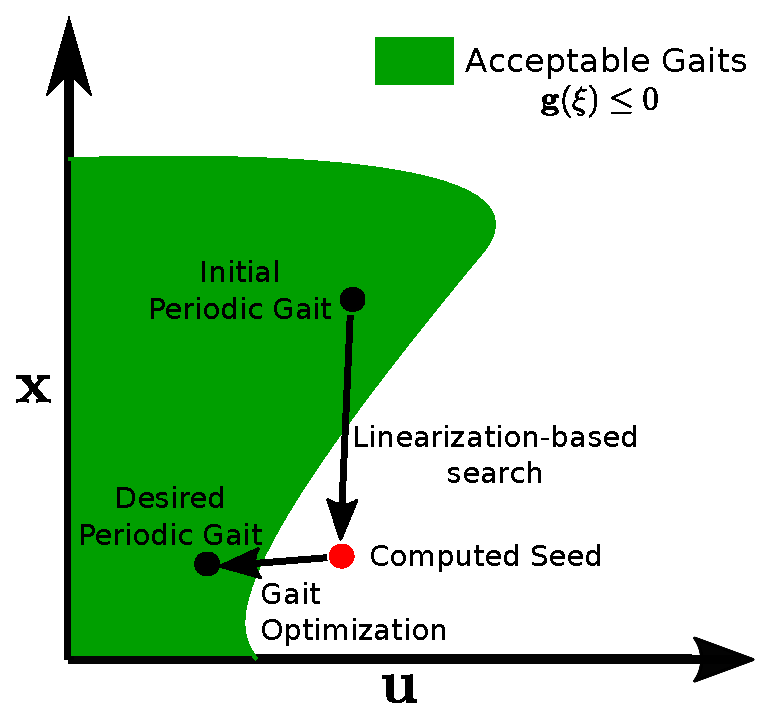
\includegraphics[width=0.5\linewidth]{homotopy.eps}
	\caption{Illustration of the linearization-based predictor-corrector search scheme to find periodic low-speed gaits}\label{fig:homotopy}
\end{figure}

Empirically, gaits at speeds greater than 0.8 m/s were found directly through optimization of \eqref{eq:gaitOpt} without special attention to initial seeds. A predictor-corrector strategy (Fig.~\ref{fig:homotopy}) was employed to address the challenges for lower velocities. In this strategy, an MS-to-MS Poincar\'e return map was linearized and used to solve for a preliminary seed during a homotopy process toward a lower-speed gait. This map is described by
%
\begin{equation}
	\x_{k+1} = \mathcal{P}(\x_k ,\u_k)
\end{equation}
%
where $\x_k$ denotes the state at MS and $\u_k$ denotes the discrete controls applied over one step as given by
\begin{align}
	\x &= \left[y_\com,\ z_\com,\ \dot{x}_\com,\ \dot{y}_\com\right]^T &
	\mathbf{u} &= \left[\phi,\ \theta,\ k\right]^T
\end{align}
The vertical velocity satisfies $\dot{z}=0$, the guard condition described in \eqref{eq:gms},  at MS. Thus $\dot{z}$ is omitted from the state $\x_k$ on the Poincar\'e surface. Following the optimization of one step of a periodic gait with state and control $\x^*_k$, $\u^*_k$, the return map is linearized providing
%
\begin{equation}\label{eq:linearized}
	\x_{k+1} \approx \x_{k+1}^* + \underbrace{\left.\frac{\partial \mathcal{P}}{\partial \x}\right|_{\x^*_k, \u^*_k}}_{:=\A} \delta \x_k + \underbrace{\left. \frac{\partial \mathcal{P}}{\partial \u}\right|_{\x^*_k, \u^*_k}}_{:=\B} \delta \u_k 
\end{equation}
%
where $\x_{k+1}^* = \mathcal{P}(\x_k^*, \u_k^*)$, $\delta \x_k = \x_k - \x^*_k$, and $\delta \u_k = \u_k - \u^*_k$. Since a gait of the 3D B-SLIP model is two-step periodic, left/right symmetry from step to step requires that $\x_{k+1}^* = \mathbf{S} \x_k^*$ where $\mathbf{S} = {\rm diag}([-1, 1, 1, 1])$. This matrix encodes that only the $y$-position of the CoM relative to the foot must change signs from step to step. Then, to solve for an approximate state/control pair for a lower-speed gait, variations to the parameters were found such that $\delta \x_{k+1} = \mathbf{S} \delta \x_k $. This constraint requires
\begin{align}\label{eq:linEq}
	\mathbf{0} = (\A-\mathbf{S})\delta \x_k + \B\delta \u_k\,. 
\end{align}

\begin{figure}
	\centering
	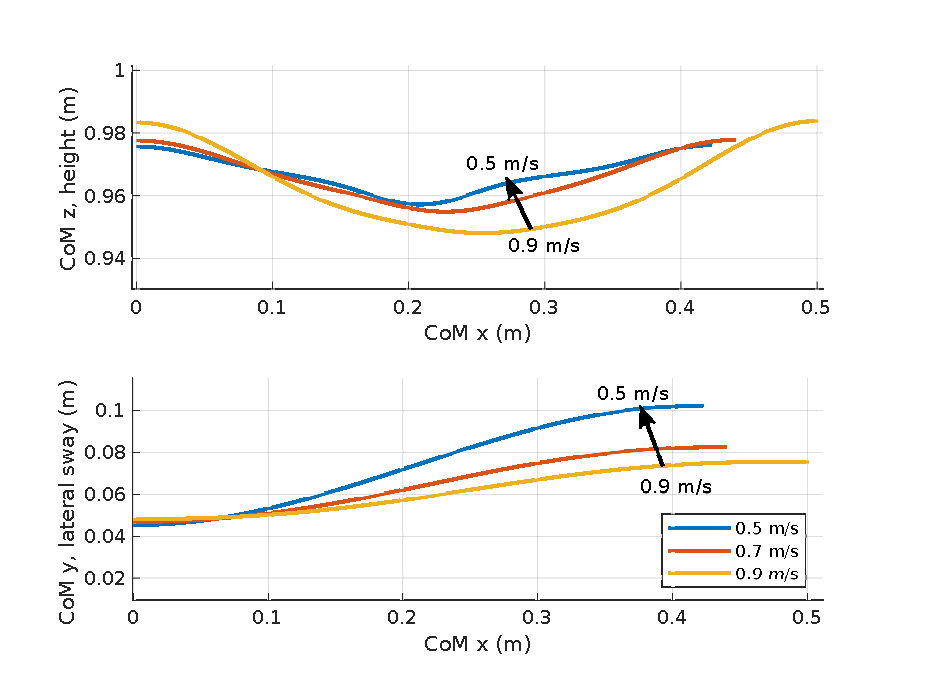
\includegraphics[width=0.8\linewidth]{subplot.eps}
	\vspace{-1em}
	\caption{A subset of the CoM trajectories in the gait library after optimization.}\label{fig:library}
\end{figure}

To generate a suitable next seed, the forward velocity component of $ \delta \x_k$ was held constant to the desired change in velocity. Considering \eqref{eq:linEq}, these equations provide 4 constraints for the 6 remaining unknowns, $ \left[\delta y_\com,\ \delta z_\com,\ \delta\dot{y}_\com,\ \delta \phi,\, \delta \theta,\, \delta k\right]^T  $, resulting in 2 degrees of freedom. Perturbations $\delta \x_k$ and $\delta \u_k$ satisfying these equations were computed with a least-norm solution, and the resulting parameters were used to seed the next gait optimization. This homotopy process was repeated until the desired low-velocity gait was optimized, resulting in a library of gaits for a range of speeds. Two libraries were generated: one at 0.4\,m/s - 0.9\,m/s for use with B-SLIP data and another at 0.6\,m/s - 1.0\,m/s for use with exoskeleton measurements, both at increments of 0.1\,m/s. As illustrated in Fig. \ref{fig:library}, generated libraries qualitatively exhibit the vertical and lateral CoM excursion trends that are observed in human data. That is vertical excursion decreases, and lateral excursion increases with a decrease in forward velocity. This linearization-based gait search method makes the generation of low-speed gaits easier and yields a library that serves as the basis for the IMM estimator outlined in the next section.

\section{Interacting Multi-Model estimation}

\begin{figure}
	\centering
	\begin{overpic}[width=0.8\linewidth,percent]{IMMblock2.pdf}
		\put(50.5,6){\textbf{\scriptsize{\eqref{eq:physicalLikelihood}},}}
		\put(50.5,3){\textbf{\scriptsize{\eqref{eq:weightCalc}}}}
		\put(72.5,4){\textbf{\scriptsize{\eqref{eq:estimates},\eqref{eq:covFuse}}}}
		\put(72.5,36){\textbf{\scriptsize{\eqref{eq:updatex}-\eqref{eq:updateP}}}}
	\end{overpic}
	\caption{IMM scheme used to estimate gait phase and walking speed.}\label{fig:IMM}
\end{figure}
The IMM is a technique to  adaptively fuse estimates from multiple filters, running in parallel. Despite their use in other hybrid systems (\cite{bar2005imm},\cite{daeipour1998imm}), the application of IMMs to legged locomotion has been minimal. One example is the use of IMMs for legged locomotion is in state estimation and gait phase prediction for RHex \cite{skaff2005context}, a six-legged robot with compliant legs. Gait phase estimation is possible by directly using force
sensors in the exoskeleton soles \cite{agostini2013segmentation,de2012gait}. However, by relating human data to template models, the presented approach may provide insight into unmeasured parameters, such as leg stiffness, and the effects of changes in them on the gait.

The IMM estimation process used in this work is illustrated in Fig. \ref{fig:IMM}. Each of the $M$ filters represents a different candidate gait and phase, and the IMM attempts to determine which of the phases is most likely. 
In what follows, $ i $ and $ j $ index over filters, and $ k$ indexes over time. There are two types of estimate interactions shown in Fig.~\ref{fig:IMM}. First, a likelihood-based mixing produces an ensemble estimate output from the IMM, while a Markov mixing relates the state estimates from the filters at time step $k$ to the initial estimates at time step $k+1$. 

The filters begin with initial state estimates $\fsup{\xh_k^0}{j}$ and covariances $\fsup{\P_k^0}{j}$ that are propagated forward to $\fsup{\xh_k^-}{j}$ and $\fsup{\P_k^-}{j}$ using the dynamics presented in \eqref{eq:sysProp} and~\eqref{eq:covProp}. Measurements from the exoskeleton sensors are used to initialize the filter at start-up and the covariance is set to be an identity matrix. The measurement likelihood ${}^j  \ell_k$ is then calculated for the state estimate of each filter as
\begin{align} \label{eq:likelihood}
	{}^j \ell_k &= p(\yt_k|\fsup{\xh_k^-}{j})  = {\rm det}( 2 \pi \fsup{\E_k}{j})^{-1/2} \,  {e}^{\lambda_r} \,~\textrm{where}\\[.5ex]
	\lambda_r &= -\frac{1}{2}\ {}^j\e_k^T \, \fsup{\E_k^{-1}}{j} \, \fsup{\e_k}{j} \nonumber
\end{align}
and $ \fsup{\e_k}{j} $ and $ \fsup{\E_k}{j} $ denote the measurement residual and its covariance, respectively, given by $ \fsup{\e_k}{j} = \yt_k - \h\!\left( \fsup{\xh_k^-}{j}\right)$ and 
\[
\fsup{\E_k}{j} = \fsup{\H_k}{j}\ \fsup{\P_k^{-}}{j}\ \fsup{\H_k^T}{j} + \fsup{\R_k}{j}. \] 
with $\fsup{\H_k}{j}$
the Jacobian of the measurement function at $\fsup{\xh_k^-}{j}$.

The measurement likelihood is then normalized across the $M$ models to calculate model weights $\fsup{w_k}{j}$ via
\begin{eqnarray}
	\fsup{w_k}{j} =  \fsup{ \ell_k}{j} \left/ \left( \textstyle\sum_{i=1}^{M} \fsup{ \ell_k}{i} \right) \right. \label{eq:weightCalc}
\end{eqnarray}
The magnitude of the weight $\fsup{w_k}{j}$ indicates the relative confidence of the filter that the system is in mode $j$ at time step $k$. In contrast to a conventional IMM approach \cite{Crassidis} where $\fsup{w_k}{j} = \fsup{w_{k-1}}{j} p(\yt_k|\fsup{\xh_k^-}{j})$, the weights from the previous iteration are not included in \eqref{eq:weightCalc}. This change was due to the fact that some likelihoods, e.g., likelihoods for DS models during SS, result in numerically zero weights, from which it is not possible to recover to non-zero weights.

Following the computation of the likelihood for each model, the noisy measurement $\yt_k$ is used with the Kalman update in \eqref{eq:kalmanGain},\eqref{eq:ekfStateUp}, and \eqref{eq:ekfCovUp} to produce \textit{a~posteriori} estimates $\fsup{\x_k^+}{j}$ and covariances $\fsup{\P_k^+}{j}$. These quantities are fused to produce an ensemble estimate $\xh_k$ with covariance $\P_k$ calculated via
\begin{eqnarray}
	\xh_k &=& \textstyle \sum_{j =1}^{M} \fsup{w_k}{j} \fsup{\xh_k^{+}}{j} \label{eq:estimates} \\
	\P_k &=& \displaystyle \sum_{j =1}^{M} \fsup{w_k}{j}  \left[\left(\fsup{\xh_k^{+}}{j} - \xh_k\right) \left(\fsup{\xh_k^{+}}{j} - \xh_k\right)^T + \fsup{\P_k^{+}}{j} \right] \label{eq:covFuse}
\end{eqnarray}
Fusion from \eqref{eq:covFuse} captures the covariance of each individual filter and of each filter estimate with the fused estimate.

Initial conditions for the next time step $\fsup{\xh_{k+1}^{0}}{j}$ are then computed considering interaction between the models as
\begin{eqnarray}\label{eq:updatex}
	\fsup{\xh_{k+1}^{0}}{j} &= \textstyle \sum_{i =1}^{M} \fsup{w_k}{(i|j)} \fsup{\xh_k^{+}}{i}
\end{eqnarray}
where  $ \fsup{w_k}{(i|j)} $ is a weight that considers a likelihood-based model probability and a Markov-based transition probability from model $ i $ to model $ j $. Markov transition probabilities $ p_{ij} $ are specified as fixed probabilities of switching from $ i $ to $ j $ and the weights are computed as
\begin{eqnarray}
	\fsup{w_k}{(i|j)} = \fsup{w_k}{i} p_{ij} / \left( \textstyle \sum_{s = 1}^{M}\fsup{w_k}{s} p_{s j} \right) \label{eq:markov}
\end{eqnarray}
Similarly, a mixed covariance for the next iteration is computed through
\begin{eqnarray}
	\label{eq:updateP}
	\fsup{\P_{k+1}^{0}}{j} &=& \sum_{i =1}^{M} \fsup{w_k}{(i|j)} \left[ \fsup{\mathbf{e}_k}{(i|j)} \fsup{\mathbf{e}^{T}_k}{(i|j)} + \fsup{\P_k^{+}}{i} \right]\,,~ \textrm{where}\\[.5ex]
	\fsup{\mathbf{e}_k}{(i|j)} &=& \fsup{\xh_k^{+}}{i} - \fsup{\xh_{k+1}^{0}}{j} \nonumber
\end{eqnarray}

\begin{figure}
	\centering
	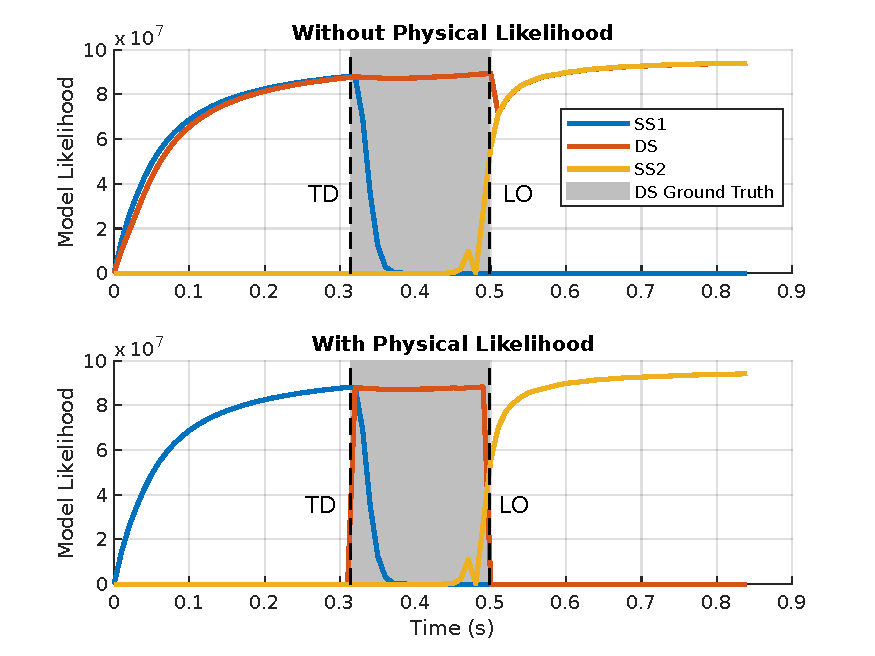
\includegraphics[width=0.75\linewidth]{likeCompare.pdf}
	\caption{The effects of the inclusion of physical likelihood on phase likelihoods}\label{fig:likeCompare}
\end{figure}

A small modification to the conventional IMM was necessary to enable the framework to correctly identify gait modes. 
The likelihood calculation \eqref{eq:likelihood} only looks at the measurement residual, which can be misleading. Dynamics during DS can track the CoM trajectories from SS data by allowing legs to extend beyond their free length, which is not physically possible. A physical likelihood term $ \lambda_p $ was added to the likelihood calculation to address this observation. This strategy takes into account the difference $\Delta l$ between the rest length and current length of the leg, which should remain positive. The likelihood is then modified as
\begin{eqnarray} \label{eq:physicalLikelihood}
	{}^j \ell_k &=& {\rm det}(2 \pi \fsup{\E_k}{j})^{-1/2}\   e^{\lambda_r + \lambda_p}\,,~\textrm{where} \\[.5ex]
	\lambda_p &=& -\kappa \min(0,\Delta l)^2  \nonumber
\end{eqnarray}
and $ \kappa>0$ is a tuning parameter. In DS, the leg with the minimum value for $\Delta l$ is used to compute $\lambda_p$.
This approach decreases the weight of a model if its estimated leg length is greater than its rest length. Figure \ref{fig:likeCompare} shows the effect this modification has on phase inference. With the change, the likelihood of DS only rises during the true DS phase, illustrated with the shaded area. The rate at which the likelihood of DS rises and decays can be tuned using $ \kappa $. With these modifications, the IMM framework can be set up to adequately identify the appropriate dynamics, SS or DS, to be used for state estimation at a given time. This IMM framework was first tested with B-SLIP simulation data and then data acquired from the EksoGT exoskeleton.

\section{Results}
%\begin{figure}
%	\centering
%	\begin{subfigure}{0.5\textwidth}
%		\centering
%		\includegraphics[width=1.1\textwidth]{posEst.pdf} % first figure itself
%		\caption{Position estimates}\label{fig:posEst}
%	\end{subfigure}\hfill
%	\begin{subfigure}{0.5\textwidth}
%		\centering
%		\includegraphics[width=1.1\textwidth]{velEst.pdf}
%		\caption{Velocity estimates}\label{fig:velEst}
%	\end{subfigure}
%	\caption{Position and velocity estimates for exoskeleton data}
%\end{figure}

\subsection{Testing with B-SLIP Simulation Data}

The B-SLIP gait used to generate synthetic measurements was from the library with a forward velocity $ \dot{x}_\com $ = 0.7 m/s. Measurements of the 3D position, forward, and vertical velocity of the CoM in the sagittal plane were used such that $ \y = [x_{\com},\ y_{\com},\ z_{\com},\ \dot{x}_{\com},\ \dot{z}_{\com}]^T $. Zero-mean Gaussian noise with constant covariance $ \R $ was added to the simulated measurements. Process noise was not added to the simulation. However, the process noise covariance $ \Q $ was retained as an estimation parameter as inaccuracies in the dynamics exist when an inaccurate gait/phase is used during estimation. The covariance values used are given by
\begin{align}
	\R &= {\rm diag}([5 ,5 ,5  ,50 ,50]) 
\times 10^{-5} \\
\Q &={\rm diag}([0,0,0,1,1,1])
\times 10^{-2}
\end{align}
where continuous process noise variances for positions and velocities are reported with units m${}^2$/s${}^2$ and m${}^2$/s${}^4$ respectively, and discrete measurement variances for positions and velocities are reported with units m${}^2 $ and m${}^2$/s${}^2$ respectively. 

\begin{figure}
	\centering
	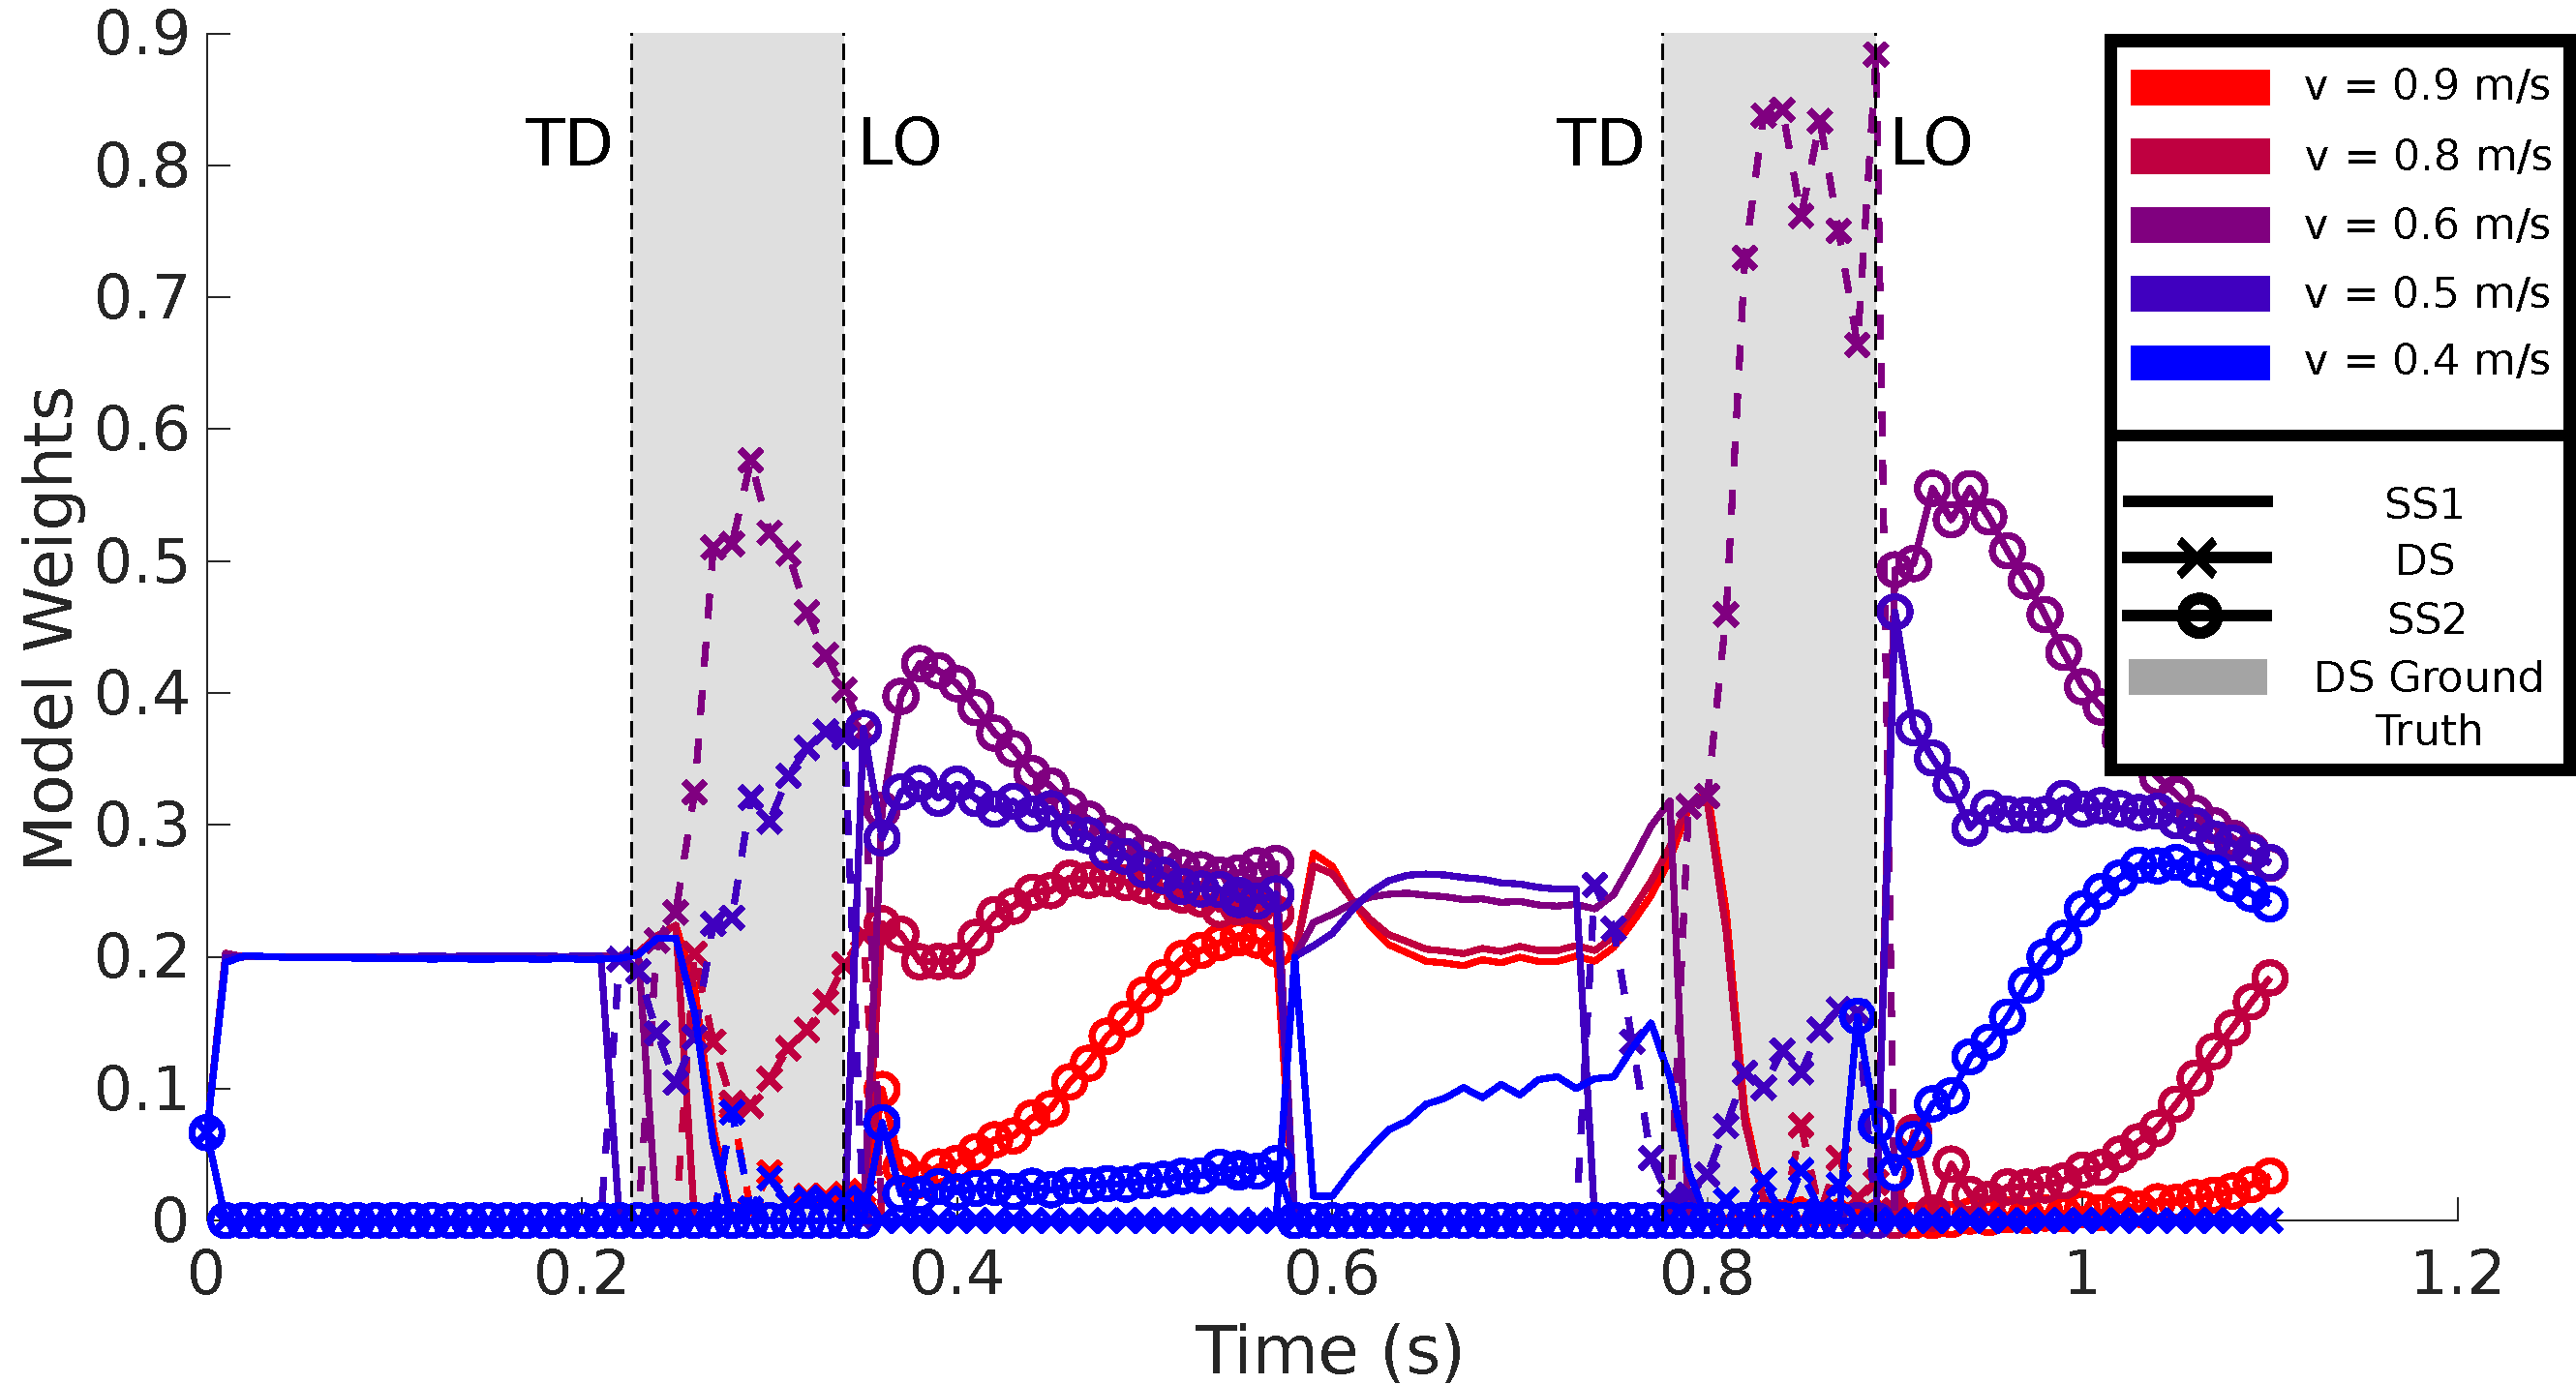
\includegraphics[width=.9\linewidth]{2StepSynth.pdf}
	\caption{Model weights output by the IMM framework applied to measurements generated from a simulation of the B-SLIP model.}\label{fig:weightSyn}
\end{figure}

Figure~\ref{fig:weightSyn} shows the weights associated with each model over two estimations cycles. The gait used to generate the measurements was excluded from the estimation library. The estimator selected the gait at $ \dot{x}_\com $ = 0.6 m/s to be the most likely as the gait that exactly matched the measurements was absent from the library. The CoM trajectories of the library gaits were similar to each other in SS1, therefore the estimator had difficulty distinguishing between them. As the gait progressed through DS, the differences in trajectories became more apparent and the estimator was able to identify the most likely gait. This may be explained by the B-SLIP model's effectiveness at describing the DS gait phase in contrast to rigid pendular models that assume an instantaneous transfer of support.

\subsection{Testing with Exoskeleton Data}

The estimation framework was then tested on data acquired from the sensors onboard the EksoGT exoskeleton during walking trials of an able-bodied person. The subject had a leg length of 0.95 m, weighed 67 kg, and walked at a self-selected speed between 0.6-0.7 m/s using crutches \cite{gambon2019characterizing}. The exoskeleton allows movement only in the sagittal plane and restricts movements in the lateral direction, however, some lateral movement of the CoM is observed due to torso roll. In addition to all the available measurements listed in Sec.~\ref{sec:exoData}, the exoskeleton also reports the estimated height and fore/aft position of the CoM in the global frame. The position of the CoM was approximated and collected in the measurement vector $ \yt = [x_\com ,y_\com ,z_\com]^T $. The evolution of the CoM state of the B-SLIP is sensitive to changes in the leg length of library gaits, particularly in the vertical direction. The parameters that defined the library gaits were rescaled with respect to the estimated CoM height of the exoskeleton user at the initial MS of the estimator trial. Additionally, the following anisotropic process and measurement noise covariances were selected.
\begin{align}
		\R &= {\rm diag}([5,5,0.5])\times 10^{-6} \\
		\Q &={\rm diag}([0,0,0,1,1,10])\times 10^{-2}
\end{align}
This covariance mitigates sensitivity by increasing the estimator's reliance on measurements and decreasing the reliance on the model when inferring vertical CoM evolution. This strategy was found to yield more accurate velocity estimates compared to isotropic covariance selection. 

\begin{figure}
	\centering
	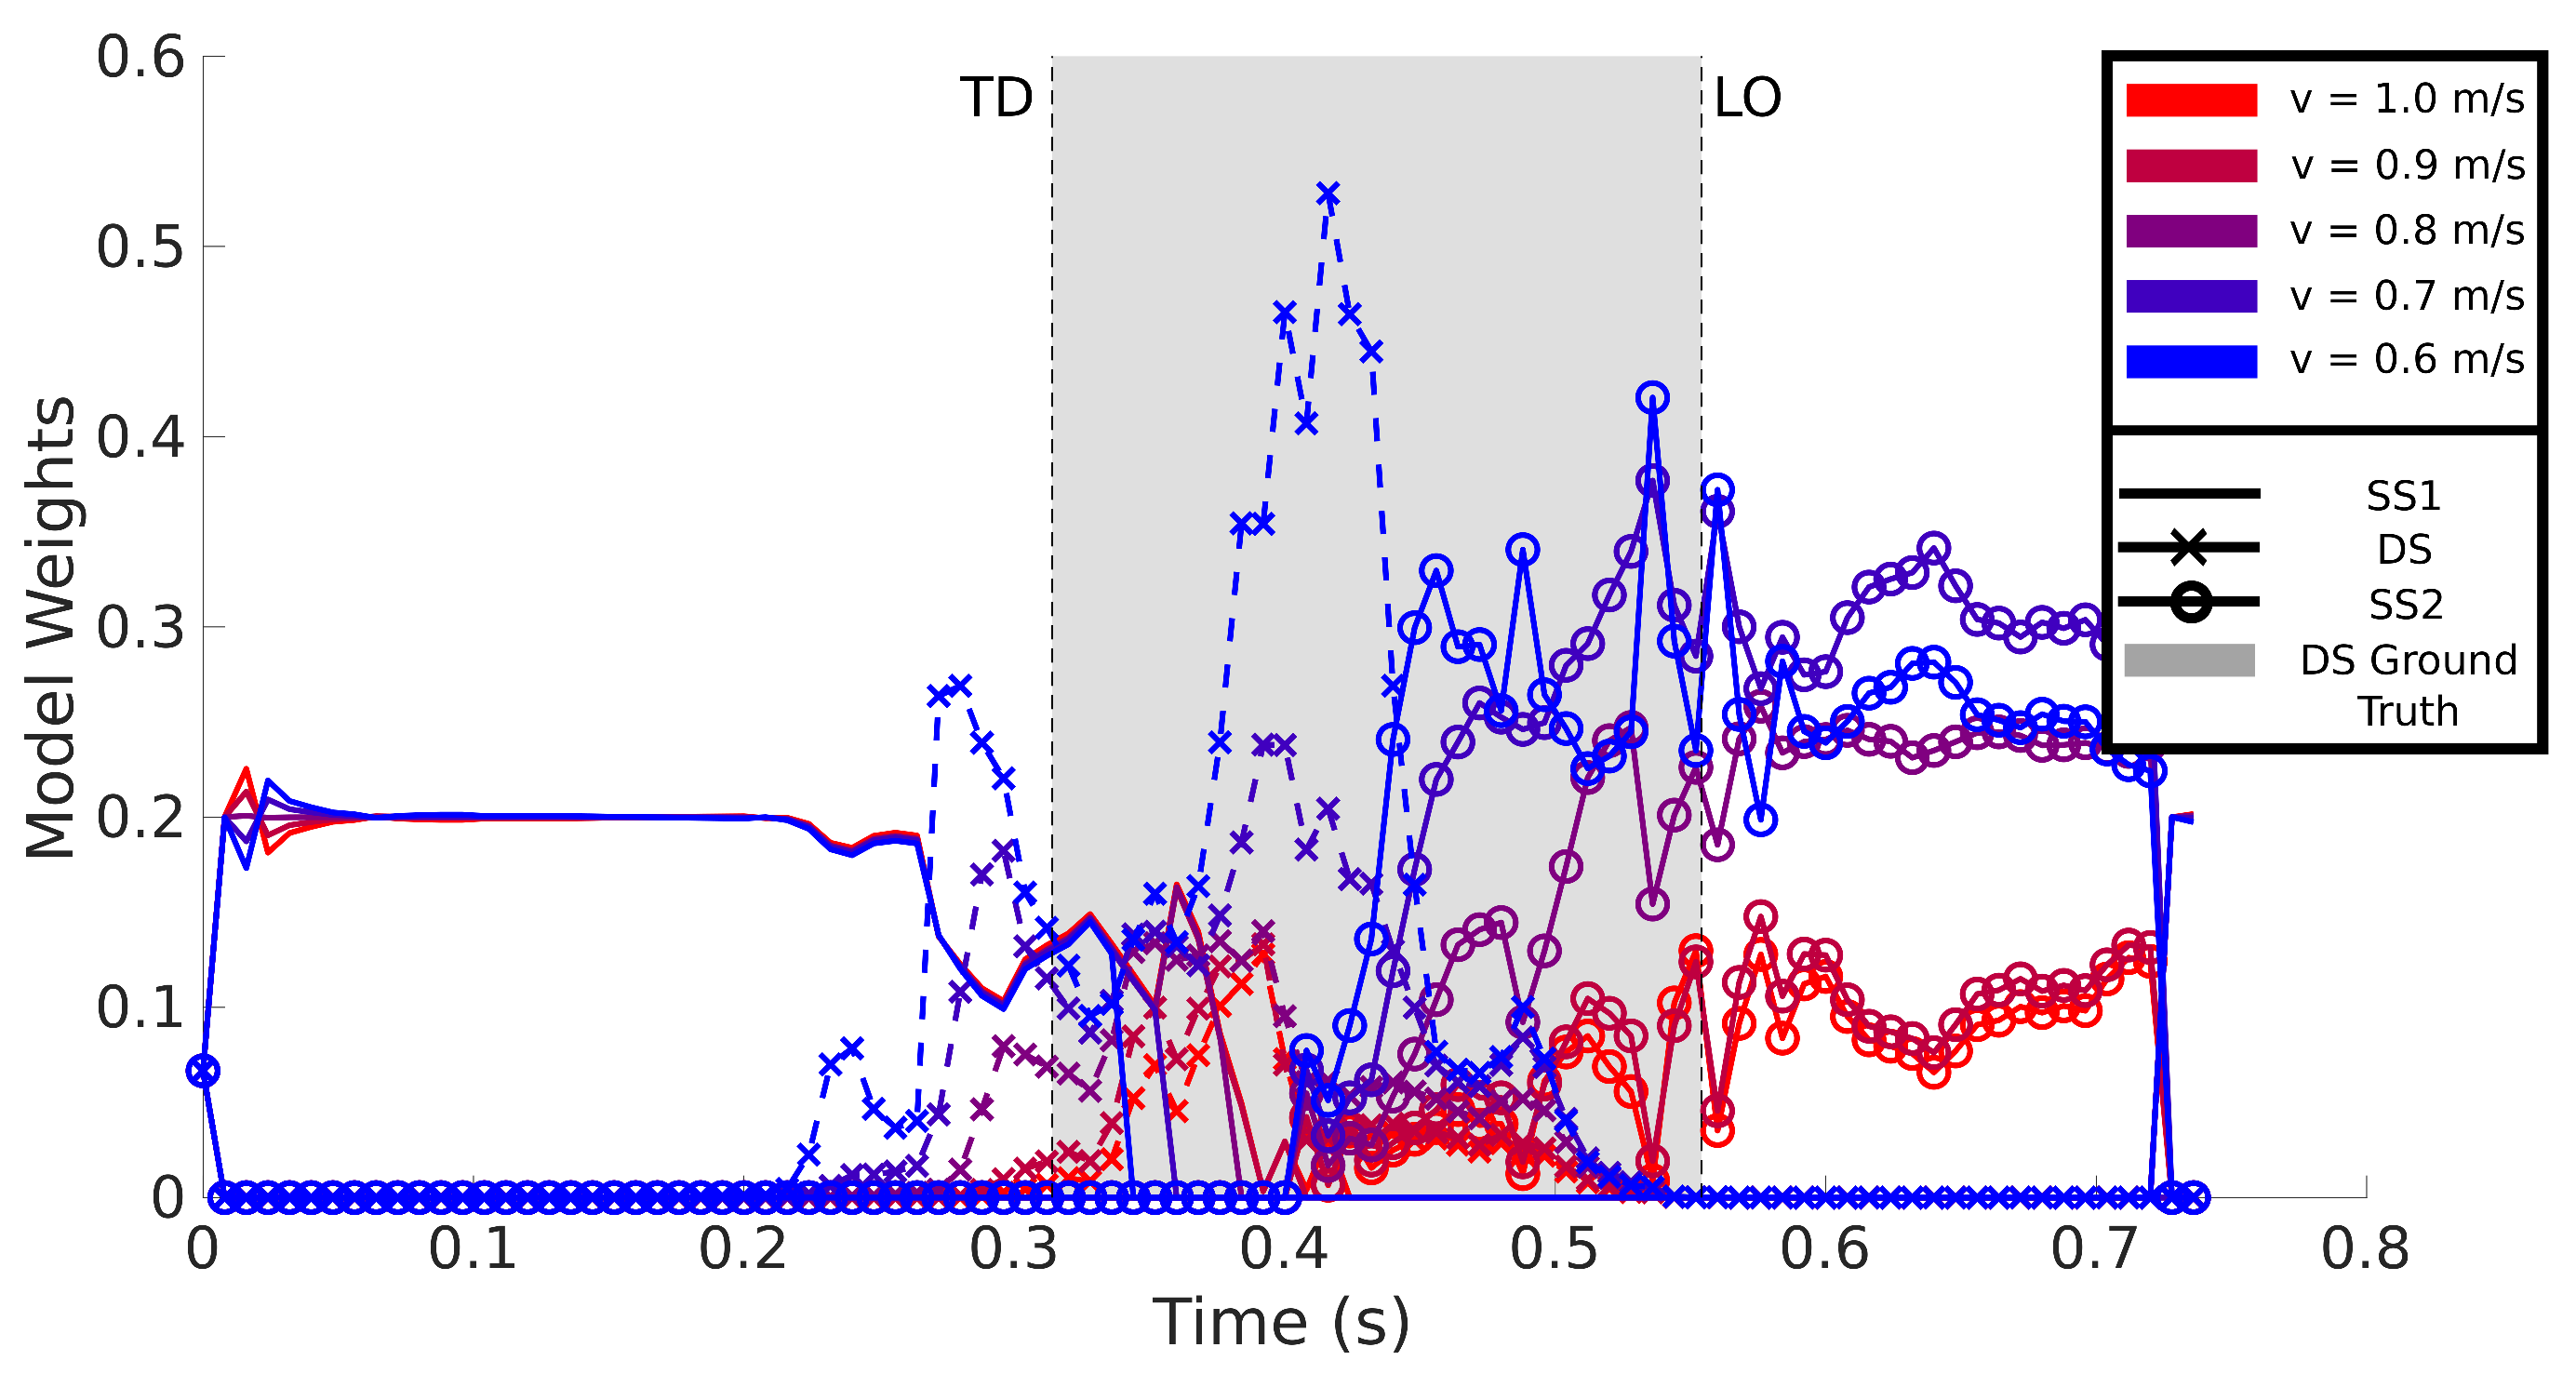
\includegraphics[width=.9\linewidth]{weightsExo.eps}
	\caption{Model weights from the IMM framework applied to experimental measurements of an able-bodied individual walking in an exoskeleton.}\label{fig:exoWeights}
\end{figure}

The most likely gaits for one step of the walking trial are illustrated in Fig.~\ref{fig:exoWeights}; higher weights indicate a more likely gait. The user was walking at a velocity between 0.6-0.7 m/s so the gaits at those speeds are shown to be most likely. All library gaits qualitatively matched human data i.e., maximum forward velocity was achieved during DS, and lateral velocity was zero at the end of the step. However, the initial and lateral positions were optimization variables when generating the gait library, and as a result, they do not match the initial position in the measured data. Therefore estimates of CoM velocities, none of which had direct measurements, took $ \approx $50 m/s to stabilize to expected behavior as illustrated in Fig.~\ref{fig:exoState} where estimates are plotted along with measured values. The DS period, illustrated in gray, was determined when foot-mounted force sensors indicated both feet were flat on the ground.
\begin{figure}
	\centering
	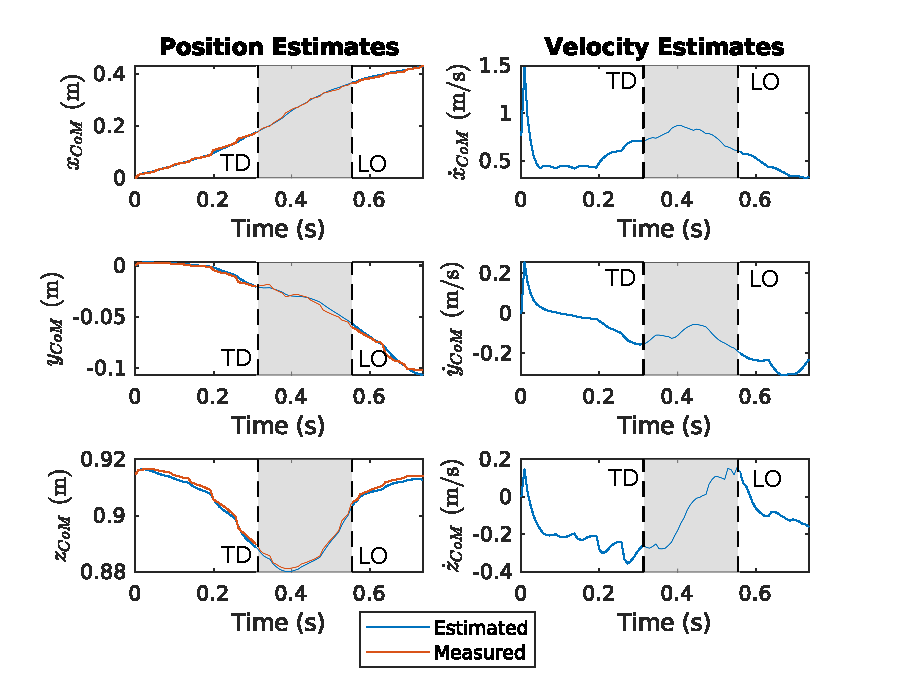
\includegraphics[width= 0.8\linewidth]{stateEstExo.eps}
	\caption{State estimates from the IMM framework applied to experimental measurements of an able-bodied individual walking in an exoskeleton.}\label{fig:exoState}
\end{figure}

\begin{figure}
	\centering
	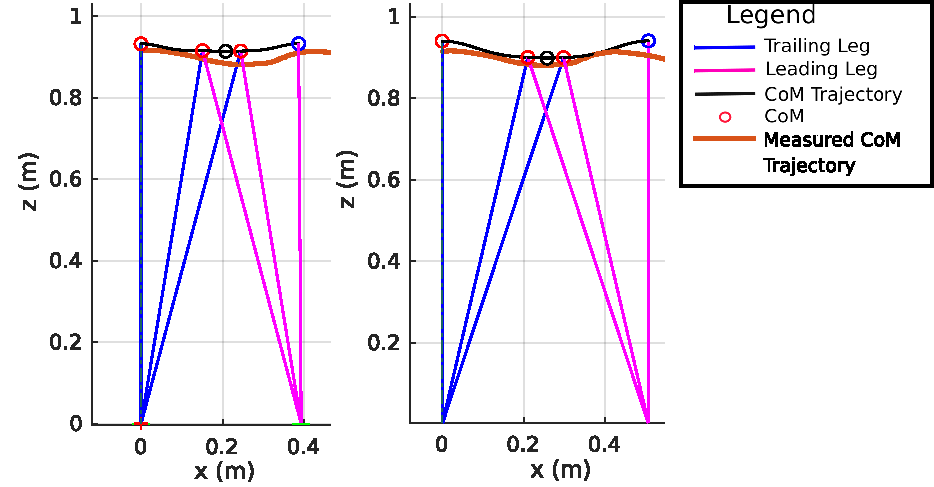
\includegraphics[width=.8\linewidth]{gaitCompare.pdf}
	\caption{Comparison of gaits at speeds of 0.6 m/s  (left) and 1.0 m/s  (right).}\label{fig:compare}
\end{figure}

The estimator relies on differences between measured CoM trajectories and simulated CoM trajectories from library gait to infer gait phase and speed. Figure 10 illustrates that while the exoskeleton user was walking at a speed between 0.6 m/s and 0.7 m/s, the CoM trajectory in the sagittal plane matches more closely with the library gait at a speed of 1.0 m/s as shown in Fig.~\ref{fig:compare}. This behavior may be due to the dynamics of walking in an exoskeleton with an ambulatory device that are not emulated by the B-SLIP model. The IMM framework was able to identify the correct gait velocity and phase of the measured data over a majority of the step despite the mismatch in trajectories. The library contains gaits at 0.6 m/s and 0.7 m/s which are indicated as most likely in Fig.~\ref{fig:exoWeights} as the user's actual gait velocity was between those two values. Thus the IMM framework functions as expected, but relies on accurate emulation of CoM trajectories from library gaits for accurate estimation.

Inaccuracies in the likelihoods of some phases were observed around phase transitions can be seen in Fig.~\ref{fig:weightSyn} and Fig.~\ref{fig:exoWeights}. This behavior is an artifact of the variety of the gait library. Computation of the physical likelihood depends on the leg length, which is the same across all library gaits. However, each of these gaits have different step lengths as the gait velocities are different. As a result, the durations of the DS phases for each of these gaits is also different. Therefore, even with the leg length rescaling, the discrepancy between the human data and library gaits causes the likelihood function to detect DS and infer the end of SS1 at different times, which causes differences in likelihood switching times. The combined state estimates of the CoM positions are still accurate to within 1cm of the measurements despite this (Fig.~\ref{fig:exoState}).

\section{Challenges with using IMMs}

\begin{figure}
	\centering
	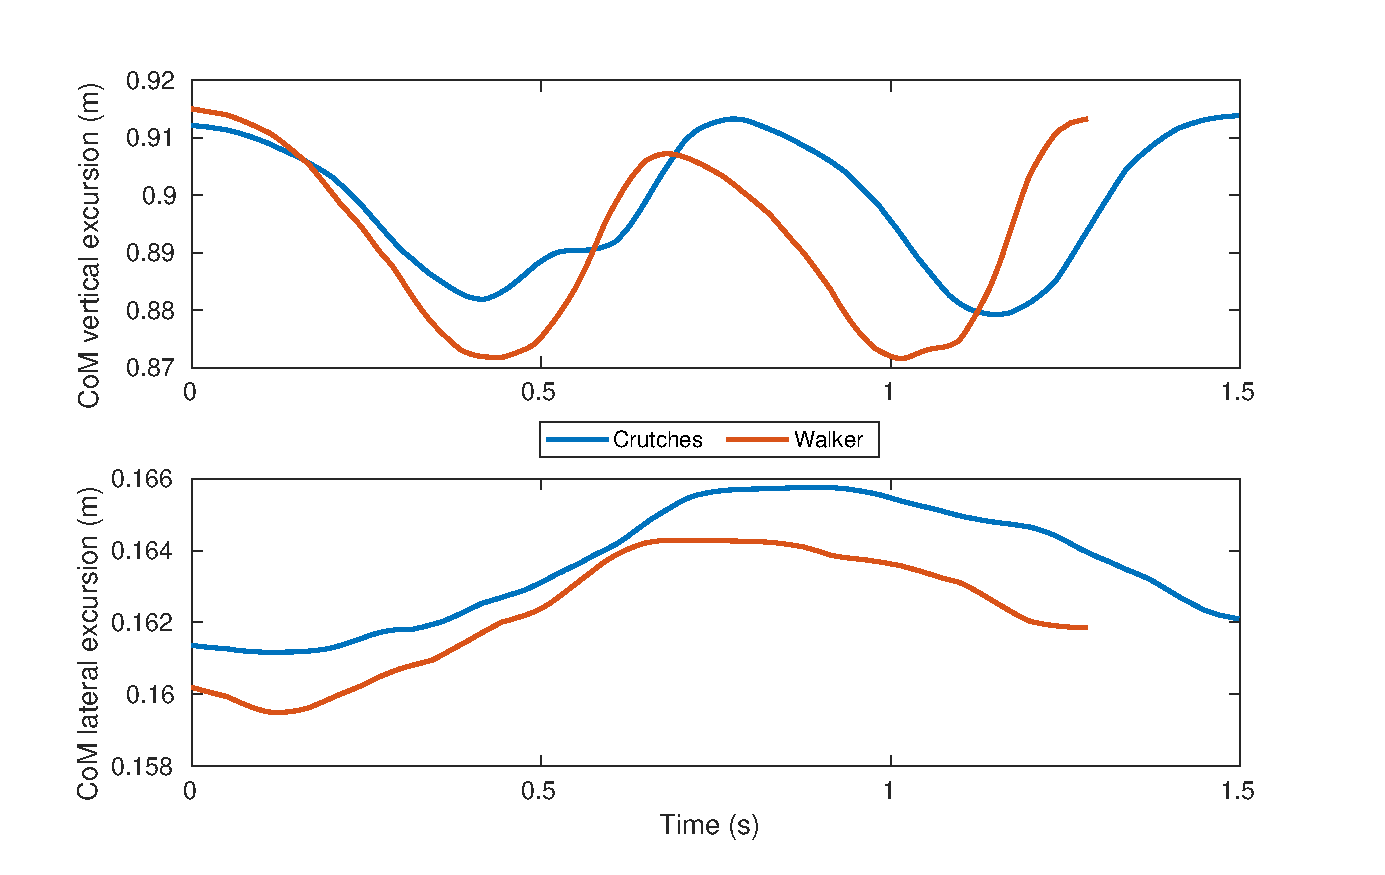
\includegraphics[width=0.9\linewidth]{trajDiff}
	\caption{CoM trajectories for two steps of the same subject walking at steady-state with a self-selected gait speed using a walker vs. crutches.}\label{fig:trajDiff}
\end{figure}
Discrepancies were observed between the measured CoM trajectories and those of B-SLIP gaits. The measured CoM trajectories are asymmetric and it is difficult to generate high-fidelity matching B-SLIP gaits. Center of mass trajectories are influenced by a variety of factors such as the choice of ambulatory device, and gait features such as gait speed, and individual joint trajectories resulting from uncoordinated limb movements. Figure~\ref{fig:trajDiff} shows the CoM trajectories of the same subject over two steps walking at steady-state using a walker and crutches. The step length and therefore, step duration, were shorter when the walker was being used resulting in considerably different trajectories. This variation in trajectories is challenging to capture using only the B-SLIP model and simply increasing the number of gaits considered by the IMM is an insufficient solution.

The ensemble estimate as calculated by the IMM (\ref{eq:estimates}) is a weighted summation of estimates from the filter library. As all gaits in the gait library are intended to match human walking, the likelihoods of the corresponding estimates will rarely go to zero. Therefore, the more gaits there are in the library, the more "polluted" the ensemble estimate will be due to irrelevant estimates being included. The implementation of the physical likelihood in \eqref{eq:physicalLikelihood} mitigates this issue between gait phases, but it does not address this issue when dealing with different filters of the same phase. A similar problem of context-based estimator selection and its scalability was addressed for legged robots by deactivating and reactivating individual filters \cite{skaff2010context} based on measurements from sensors onboard the robot. However, this approach may not capture the variability observed in human walking.

\section{Summary}
This chapter shows that the IMM framework is capable of estimating an exoskeleton user's intended gait and phase by comparing measured CoM trajectories of exoskeleton users to simulated B-SLIP gaits. The  quality of these estimates is highly dependent on the quality of the underlying gait library as the estimation relies solely on matching CoM trajectories. Changes in the individual gait variables add up to influence CoM trajectory. It may not always be possible to predict these changes with a simple template model such as the B-SLIP, therefore, the IMM framework may be used as a high-level framework that may be supplemented by another estimator to monitor the individual gait features that affect CoM trajectories. The reactive nature of this framework may also be addressed by considering these gait features and relating them to changes in gait velocity.
	%
	% BKF
	\chapter{Intent Change Estimation Based on Physical Interactions of an	Exoskeleton User}\label{chapter:BKF}
The IMM estimation framework presented previously is reactive as it monitors signs of gait transition i.e.~if the CoM trajectory after gait transition does not resemble library gaits, the IMM algorithm will misidentify the intended change until after it has been realized. However, anticipative intent inference is more desirable to time the assistance delivery appropriately and help the user realize their intended gait transition. Improper assistance timing may result in the robot resisting the user's actions, hampering HRI fluency. Intent may be anticipatively inferred by identifying the actions the user takes to realize their intent change and using data from gait features to detect them. Actions indicative of intent change may be detected by monitoring the interactions the user has with the exoskeleton and the environment. These interactions may provide an earlier indicator of intent changes compared to CoM or joint motions making it possible to anticipate user intent and provide assistance to the user to help realize the desired objective. 

\section{Quantifying intent - Enabling estimation}
User intent is an abstract content, so it must be quantified and inferred using a measurable quantity, and this quantification is a design choice. The intended gait speed was chosen to represent user intent as the primary objective of the exoskeletons herein is gait rehabiliation. Estimating the gait speed of an individual may increase the possibility for finer control of the gait and also limit the need to train for multiple discrete scenarios. The state of the exoskeleton user is represented in a vector \[\x = [\mathbf{p}_{CoM}^{\top} ,\mathbf{v}_{CoM}^{\top}]^{\top} \] 
To capture intent, the state was extended to include the intended gait velocity $ z $ as a hidden state in an augmented state vector $ \q = [\x^{\top} ,z]^{\top} $. The gait velocity $ v_x^d $ only represents the velocity in the sagittal plane. Velocity in the transverse \footnote{The transverse plane is the plane that divides the body into top and bottom parts. } plane (e.g., while turning) is neglected, as the exoskeleton restricts adduction/abduction of the legs. This state augmentation approach allows using the Kalman filter to directly estimate the intended gait speed. 

Previously performed studies of bipedal locomotion give us an idea of how changes in walking gaits corresponding to transitions in user intent. These physical indicators include differences in CoM trajectories and foot placement, as illustrated in Fig.~\ref{fig:main_idea}. Ground contacts greatly influence the stability of legged locomotion, so it was hypothesized that intent will be reflected strongly in the user's choice of ground contacts through foot placement \cite{bhounsule2014foot}. Modulating foot placement while walking is an effective control mechanism to maintain stability \cite{hof2010balance,bhounsule2015control}, and it has been shown that velocity changes at MS influence foot placement at TD \cite{wang2014stepping,redfern1994model}. 

\begin{figure}
	\centering
	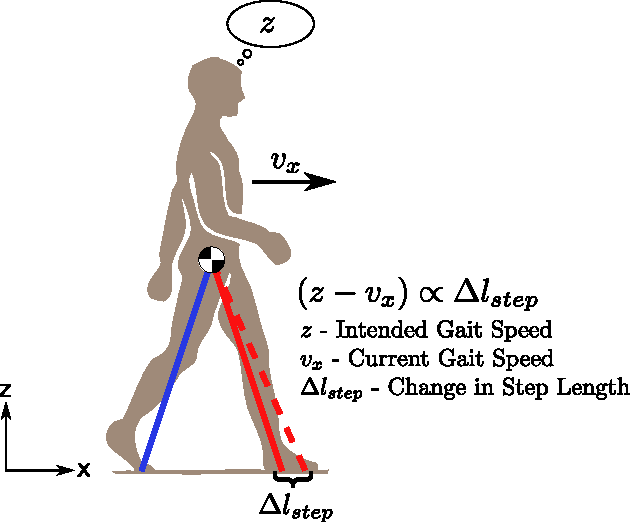
\includegraphics[width=0.5\linewidth]{main_idea}
	\caption{Change in intended velocity may be inferred from change in step length}\label{fig:main_idea}
\end{figure}

The B-SLIP model may be used to adequately model steady-state walking, and foot placement was found to be critical in optimizing periodic gaits. The model does not inherently capture the active changes required to change speed nor the first-principles humans employ for foot-placement as a function of the desired gait speed. These aspects were initially modeled by designing a controller for the B-SLIP model to emulate human motor control. With such a design, intent changes may be considered analogous to controller setpoint changes. Several theories try to explain human motor control, one of which says that the human sensorimotor system relies on optimal control \cite{todorov2004optimality,sylla2014assessing}. Therefore, we chose to assume the human motor controller to be a Linear Quadratic Regulator (LQR). The MS-to-MS Poincar\'e map was linearized about a periodic gait and the linearized model was used to design a controller that minimized deviations from a specified gait. 

The dynamics of the B-SLIP model are nonlinear and linearizing them about a single periodic gait results in a model valid for a very small portion of the gait which rendered the controller unable to handle large speed changes. A derivative-free technique i.e., the Unscented Transform \cite{manchester2016derivative} were employed to generate a linear model. This technique required integrating dynamics backward in time which was difficult to do for the hybrid dynamics of the B-SLIP model as the gait event timing cannot be fixed. Therefore, due to the lack of first principles that describe human choices to bring about intended gait changes, a data-driven approach was chosen to model the relationship between intended gait speed and foot placement.

\begin{figure}
	\centering
	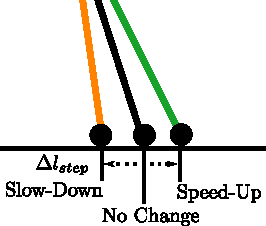
\includegraphics[width=0.35\linewidth]{step_change.pdf}
	\caption{Speed-up and slow-own increase and decrease the step length respectively}\label{fig:step_change}
\end{figure}

There is a correlation between step length and walking velocity that can be exploited to infer changes in intended gait speed. People walking at lower velocities exhibit shorter step lengths, and an increase in velocity results in an increase in step length \cite{kuo2001simple,andriacchi1977walking}, as illustrated in Fig.~\ref{fig:step_change}. Such a velocity-step-length relationship can also be viewed as valid assuming that the walk ratio is roughly constant \cite{sekiya1997optimal}. 

The walk ratio, defined as the ratio of the step length to cadence~\cite{rota2011walk}, is fairly invariant with respect to gait speeds for community ambulation, i.e.,~gait velocities greater than 0.8 m/s, despite age and terrain. It is affected when attention is divided between motor and cognitive tasks i.e., dual-task walking \cite{bogen2018walk}. The walk ratio increases as speed decreases below community ambulation velocities \cite{murakami2017estimated} and is dependent on the nature and severity of injuries \cite{rota2011walk} during unassisted walking. In rehabilitation, the variability in the walk ratio may be reduced due to the stability provided by the exoskeleton structure and consistent timing of the exoskeleton assistance \cite{seo2015new}. While the effects of exoskeleton-assisted walking on the walk ratio remain open, this analysis suggests that it is reasonable to assume a constant walk ratio for the work herein.

\section{Framework to estimate desired gait speed - Buttressed Kalman Filter}

It was assumed that intent changes made at the first MS are reflected in the placement of the foot at TD and then maintained as constant until the subsequent MS. As illustrated in Fig.~\ref{fig:step_stages}, a step starts at MS, the footstep is finalized at TD, and the step is completed at the next MS. Therefore, a twice-per-step strategy that relies on a simple model to exploit the relationship between velocity change and step length change was used to estimate intent at TD and MS. 

\begin{figure}
	\centering
	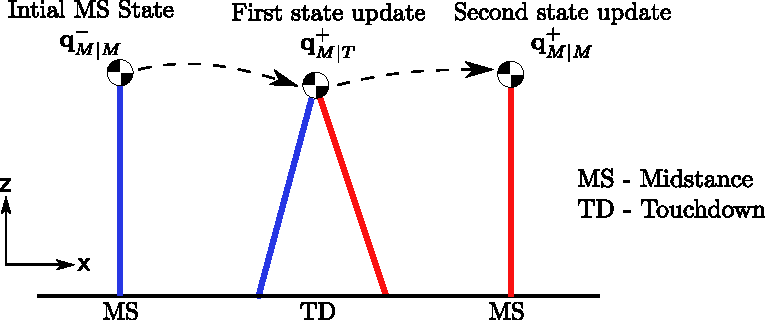
\includegraphics[width=0.75\linewidth]{step_stages.pdf}
	\caption{Two-stage estimation process}\label{fig:step_stages}
\end{figure}

A staged estimation scheme, as illustrated in Fig.~\ref{fig:block_diag}, was considered to infer intent changes using step length change information. The unit delay represents the passing of estimates as initial conditions for the next estimation cycle. In this scheme, footstep information at TD was first used to update the intent state for the initial MS. The position and velocity of the CoM were then corrected with a second update at the terminal MS of the step. A simple data-driven model of step length was used as a function of the velocity $ v_x $ at the MS prior to TD, desired velocity $ z $, and leg length $ l_{leg} $:

\begin{equation}
	l_{step} = [v_x\ (z-v_x)\ l_{leg}] \greekvec{\kappa} \label{eq:stepModel},
\end{equation}
where $ \greekvec{\kappa} $ is a vector containing regression coefficients and the model output is a scalar value in meters. This model takes into consideration the nominal step length as a function of leg length, the current velocity, and desired velocity.

\begin{figure}
	\centering
	\begin{overpic}[width=0.7\linewidth,percent]{block_diagram}
		\put(12.7,11){\scriptsize Eq.~\eqref{eq:sig_yy} - \eqref{eq:tdCovUp}}
		\put(47,11){\scriptsize Eq.~\eqref{eq:model} - \eqref{eq:P_up}}
	\end{overpic}
%	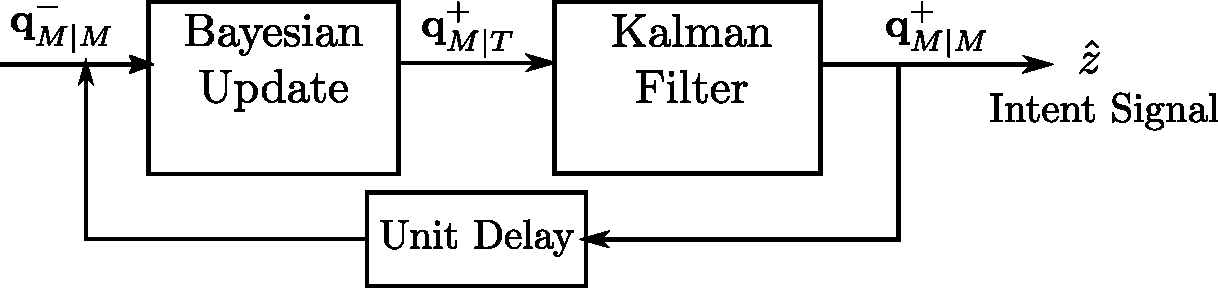
\includegraphics[width=0.7\linewidth]{block_diagram.pdf}
	\caption{Twice-per-step strategy to estimate user intent}\label{fig:block_diag}
\end{figure}

This estimation strategy is briefly  where  

The step length model may be used as a measurement model in a Kalman filter framework to relate the intended gait speed to the measured step length. The estimator operates on the the state $ \hat{\q} $ and its covariance $ \P $. In the following equations, the superscripts $ - $ and $ + $ denote pre-/post-update states respectively, the subscripts $ M $ and $ T $ denote MS and TD respectively, and the bar denotes the update location. For instance, $\hat{\q}_{M|T}^+ $ represents the state of the CoM at MS updated at TD. 

Since the footstep model is data-driven and may have inaccuracies, a process noise covariance $ \Q_{T} $ was added to the state estimate covariance $ \P^-_{M|M} $. Additionally, the estimated measurement covariance $ \Ssigma_{yy} $ was computed using the Jacobian of the measurement model $ \H_{T} $ and measurement covariance $ \R_{T} $. The predicted step length from Eq.~\eqref{eq:stepModel} was compared to the measured step length $ \tilde{\y}_{T} $. The state at MS $ \hat{\q}_{M|M}^- $ and its covariance were then updated using a Bayesian update as shown in Eq.~\eqref{eq:tdUp} and Eq.~\eqref{eq:tdCovUp}.

\begin{eqnarray}
	\hat{\y}_{T} &=&  l_{step}(\hat{v}_x,\hat{z}, l_{leg}) \nonumber \\
	\H_{T} &=& \left. \frac{\partial \hat{\y}_{T}}{\partial \q}\right|_{\hat{\q}} \nonumber \\
	\Ssigma_{yy} &=& \H_{T} \left(\P^-_{M|M} + \Q_{T}\right) \H_{T}^{\top} + \R_{T} \label{eq:sig_yy}\\
	\hat{\q}_{M|T}^+ &=& \hat{\q}_{M|M}^- + \P^- \H_{T}^{\top} \Ssigma_{yy}^{-1} (\tilde{\y}_{T} - \hat{\y}_{T})  \label{eq:tdUp}\\
	\P^+_{M|T} &=& \P^-_{M|M} -\P^-_{M|M} \H_{T}^{\top} \Ssigma_{yy}^{-1} \H_{T} \P^-_{M|M} \label{eq:tdCovUp}
\end{eqnarray}

This update to the previous MS state using TD information then primes $ \hat{\q}_{M|T}^+ $ and $ \P^+_{M|T} $ to be used with a Kalman filter.	Simple dynamics are used to propagate this state and covariance to the next MS 
\begin{eqnarray}
			\hat{\q}_{M|T}^+ &\leftarrow& \D \hat{\q}_{M|T}^+ \label{eq:model}\\
			\P^+_{M|T} &\leftarrow& \D  \P^+_{M|T} \D^{\top} + \Q_{M} \label{eq:cov}
\end{eqnarray}

These simple dynamics change the signs of the lateral position and velocity of the CoM to emulate the switching of the stance foot and allow for the application of a standard Kalman filter from MS to MS. It is assumed that the motion of the CoM is periodic with respect to the stance foot; however, since the CoM position is referenced from the stance foot, which changes step to step, the lateral position and velocity also change signs. Therefore, the propagation matrix is $ \D = {\rm diag}([1 ,-1 ,1 ,1 ,-1 ,1 ,1]) $. 

The second update takes place at the next MS, with the stance foot switched. The outputs of Eq.~\eqref{eq:model} and \eqref{eq:cov} are updated using a Kalman update 
\begin{eqnarray}
	\K &=& \P^+_{M|T} \H_{M}^{\top} \left(\H_{M} \P^+_{M|T} \H_{M}^{\top} + \R_{M}\right)^{-1}\\
	\hat{\q}_{M|M}^+ &=& \hat{\q}_{M|T}^+ + \K(\tilde{\y}_{M} - \H_{M} \hat{\q}_{M|T}^+) \\
	\P^+_{M|M} &=& (\I - \K \H_{M}) \P^+_{M|T} \label{eq:P_up}
\end{eqnarray}
where the measurement model Jacobian is $ \H_{M} = \I^{6\times7} $ since the measurements are $ \tilde{\y}_{M} = [\tilde{\p}_{CoM} ,\tilde{\v}_{CoM}]^{\top} $.


	%
	% Model Personalization
 	\chapter{Personalization of Gait Speed Estimation in the Presence of Data Scarcity}\label{chapter:MP}

The BKF framework presented in the previous chapter was able to anticipatively estimate changes in the user's desired gait speed. Anticipative estimation can enable the exoskeleton to better react to the user's desire to change speed and react accordingly. Additional analysis showed that estimator performance can be improved by increasing the number of gait features considered in the BKF. As a result, the work presented in this chapter considers measurements from 18 gait features in the estimation framework. Additionally, this chapter describes a data pooling process to increase the amount of available training data while maintaining the user-specific nature of the estimator, and the resulting improvements in estimator performance. 

Gait patterns of people with iSCI exhibit higher inter-subject variability than uninjured people \cite{sohn2018variability}, which creates the need for personalized exoskeleton assistance to better suit each user. Personalization may better accommodate the increased intra-subject variability because of spastic disturbances resulting from iSCIs~\cite{krawetz1996gait}. Tucker et al.~\cite{tucker2020preference} further highlight the benefits of personalizing exoskeleton assistance by giving the user pairwise options to modify exoskeleton control parameters and increase comfort. While controller personalization is important for comfort, the personalization of intent estimation represents a complementary area of need for HRI fluency.

One of the challenges of effective personalization is the prohibitive amount of training data required. As there is a limited amount of data for exoskeleton-assisted walking, the work presented in this chapter aims to address that scarcity by fusing user-independent trial data from uninjured users with user-specific data from novel users (Fig.~\ref{fig:main_idea_mp}).
The main idea of this approach is that gait feature trends exhibit similarities across subjects, e.g., step length and frequency increase with speed. The estimator personalization developed in this work seeks to exploit these similarities and create a base dataset from uninjured subjects. As people with iSCIs are expected to show similar gait feature trends, this dataset may then be transformed to provide additional training data for them. Similar ideas of exploiting gait feature commonalities has previously been used to develop user-independent gait mode estimation approaches for healthy individuals \cite{kilmartin2009optimising,ibrahim2008gait}. 

\begin{figure}
	\centering
	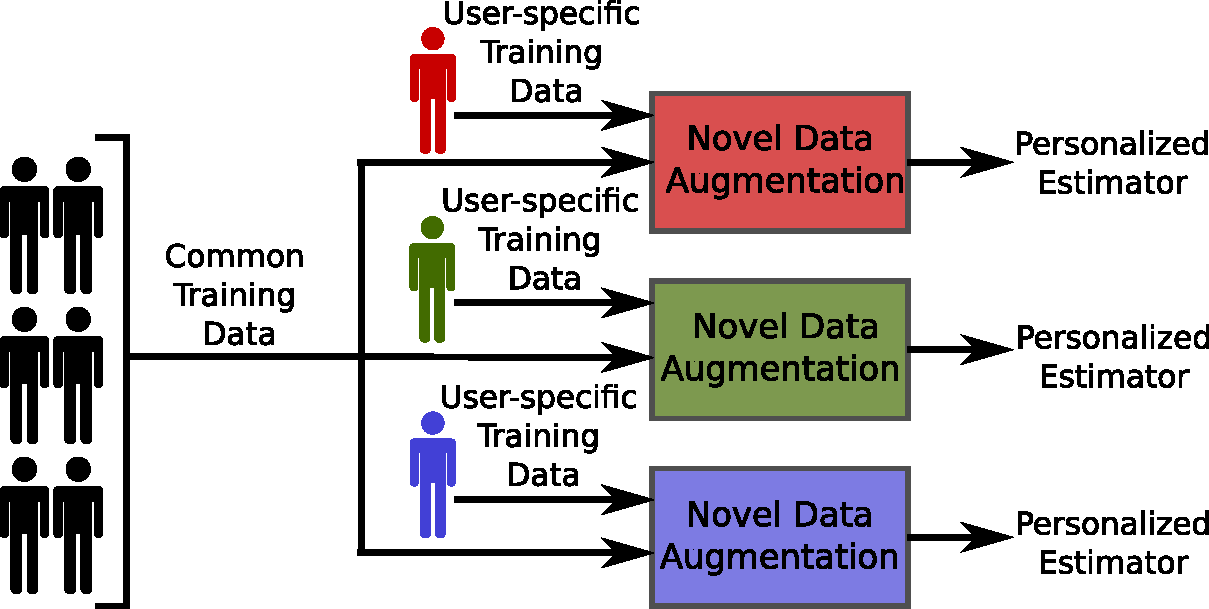
\includegraphics[width=0.7\linewidth]{main_idea_mp.pdf}
	\caption{Estimator personalization by using base and user-specific novel data from walking trials in the EksoGT exoskeleton.}\label{fig:main_idea_mp}
\end{figure}

User-independent intent detection strategies for powered prostheses are also relevant to the goals of this study, since prosthesis control strategies must address similar HRI challenges. There is very little work regarding user-independent intent recognition for powered prostheses and even less for exoskeleton-assisted walking for individuals with iSCIs. User-independent prediction of gait mode for prosthesis users has been implemented using Linear Discriminant Analysis (LDA) \cite{young2013classifying}, Dynamic Bayesian Networks (DBNs) \cite{young2015classification}, and gradient boosted decision trees \cite{bhakta2020machine} with each method showing improvement over the last. These methods rely on EMG or mechanosensory data, however, a gait-mode estimator based on 3D imaging of foot placement has also been shown to produce accurate results \cite{massalin2017user}. 

A majority of the state-of-the-art work referenced previously considers the problem of activity classification, i.e., detecting walking on flat ground, ascent/descent on ramps and stairs. The objective of the work presented in this chapter, similar to Chapter~\ref{chapter:BKF}, is to capture intent changes through changes in intended gait speed. This objective, coupled with the gait variability seen in exoskeleton walking, means there is difficulty in obtaining labeled training data about changes in intended speed as compared to changes in activity. This shortage of training data increases the difficulty of developing estimators that can identify changes in intended gait speed. Further, while there is some initial previous work regarding continuous speed estimation for prostheses \cite{best2021phase}, no such work is available regarding exoskeleton-assisted walking.

Despite inter-subject gait variability, common patterns relating gait changes to speed changes are observed across users. For example, step length and frequency, pitch and roll motions of the torso, and joint angle trajectories all show qualitatively similar trends relating to speed changes across individuals. The main contribution of this work is a method to personalize the estimation of the gait speed for subjects with SCIs walking in a lower-limb exoskeleton. The proposed method addresses training data scarcity by supplementing novel user data with transformed gait data collected from trials of uninjured users. 

While the work presented herein uses the BKF, its formulation was revised to help improve accuracy. The models used in the estimator proposed in Chapter~\ref{chapter:BKF} were trained using data from a single subject. In contrast, the work presented in this chapter explores how to incorporate data from multiple subjects to generate the necessary models, while retaining personalization for new users. Additionally, the work presented herein explores the effects that the user's choice of assistive ambulatory device, a walker or crutches, has on the personalized estimator.

%The primary contribution of this work to address data scarcity is a method to pool data from walking trials of uninjured and injured users. 
This chapter is organized as follows. Section~\ref{sec:mp_transform} describes the transformation of base data from uninjured subjects to match the distribution of the novel data form injured subjects and enable pooling. This pooling can be achieved via a variety of combinations of base and nove data. Section~\ref{sec:MI} describes a strategy to choose the appropriate combination of novel and base data using the Mutual Information between measurements of gait features and gait speed and Section~\ref{sec:models} describes the conditional Gaussian models used in the first stage of the revised formulation of the BKF. The performance of the method for crutch and walker-assisted walking was evaluated on experimental data, as discussed in Section \ref{sec:results}. This chapter describes the results reported in a previous journal publication \cite{karulkar2022personalized}.

\section{Methods} 
One of the difficulties in using learning-based strategies is the shortage of training data. There are multiple datasets of walking trials of uninjured individuals \cite{hu2018benchmark,anguita2013public,fukuchi2018public} however there is a lack of data from walking trials of exoskeleton users. This problem is further complicated by the coupling present in human-robot dynamics as each user may interact differently with the robot \cite{sylla2014assessing}. This variability increases when considering different ambulatory devices \cite{gambon2019characterizing} or injury severity \cite{gambon2020effects, rota2011walk}. Therefore, it is important to develop a method that may address the data scarcity in exoskeleton-assisted walking by enabling the re-use of training data across multiple users.

\subsection{Novel User Data Augmentation}

Combining base and novel data is a two-step process. This first step (Section~\ref{sec:mp_transform}) is to transform the distribution of the base data so its mean and covariance match that of the distribution of the novel data. The second step (Section~\ref{sec:MI}) is to choose the appropriate combination of novel and base data to ensure that the exoskeleton user's gait patterns are well represent in the pooled data.

\begin{table}
	\footnotesize
	\centering
	\caption{Gait features considered for desired gait speed estimation }\label{table:features}
	\setlength\extrarowheight{2pt} 
\begin{tabularx}{\linewidth}{|C|C|}
	\hline
	\textbf{Gait Feature}	& \textbf{Description} \\
	\hline
	Step Length (m)	& Step length as computed at TD \\
	\hline
	RMS Swing Current - Hip (A)	& Swing leg hip motor - MS to TD \\
	\hline
	RMS Swing Current - Knee (A) & Swing leg knee motor - MS to TD \\
	\hline
	Time-to-TD (s)	& Time from MS to TD - proxy for step frequency \\
	\hline
	Hip Angle - Swing (rad)	& Hip angle of the swing leg at TD \\
	\hline
	Knee Angle - Swing (rad)	& Knee angle of the swing leg at TD \\
	\hline
	Hip Angular Velocity - Swing (rad/s) & Hip joint velocity - swing leg at TD \\
	\hline
	Knee Angular Velocity - Swing (rad/s)	&  Knee joint velocity - swing leg at TD \\
	\hline
	Hip Angle - Stance (rad) & Hip angle of the stance leg at TD \\
	\hline
	Knee Angle - Stance (rad) & Knee angle of the stance leg at TD \\
	\hline
	Hip Angular Velocity - Stance (rad/s) & Hip joint velocity - stance leg at TD \\
	\hline
	Knee Angular Velocity - Stance (rad/s) & Knee joint velocity - stance leg at TD \\
	\hline
	Torso Pitch Angle (rad)	&  Angle with the vertical in the sagittal plane\\
	\hline
	Torso Pitch Angular Velocity (rad/s) & Angular velocity in the sagittal plane \\
	\hline
	Torso Roll Angle (rad) &  Angle with the vertical in the frontal plane \\
	\hline
	Torso Roll Angular Velocity (rad/s)	& Angular velocity in the frontal plane  \\
	\hline
	Leg Angle (rad) & The angle made with the vertical by the line connecting the estimated CoM and leading foot position at TD \\
	\hline
	Leg Angle (rad) & The angle made with the vertical by the line connecting the estimated CoM and leading foot position at TD \\
	\hline
	Current gait speed (m/s) & The gait speed measured at MS \\
	\hline
\end{tabularx}
\end{table}

\subsubsection{Transforming Data from Uninjured Users to Match Novel Data} \label{sec:mp_transform}
Measurements from sensors onboard the exoskeleton were used to compute eighteen gait features ($S=18$) listed in Table~\ref{table:features} for use in the estimator. Data from healthy users walking in an exoskeleton may be easily obtained to satisfy the requirements of data-driven methods. These data still retain high-level similarities in gait feature trends (e.g., changes in step length with changes in gait speed \cite{karulkar2021using}). This commonality between gait patterns may be exploited to augment the amount of available training data for injured users.

Gait feature and gait speed measurements were found to be well approximated with Gaussian distributions \cite{austin2011disambiguation}. This assumption to use Gaussian distributions was further justified by the analysis of gait feature and gait speed measurements. Figures \ref{fig:v_dist} and \ref{fig:sl_dist} show the histogram of the changes in measured gait velocity and step length for IU-1 along with fitted normal distributions. These measurements were used in the selection of the appropriate novel/base pairing. 

\begin{figure}
	\centering
	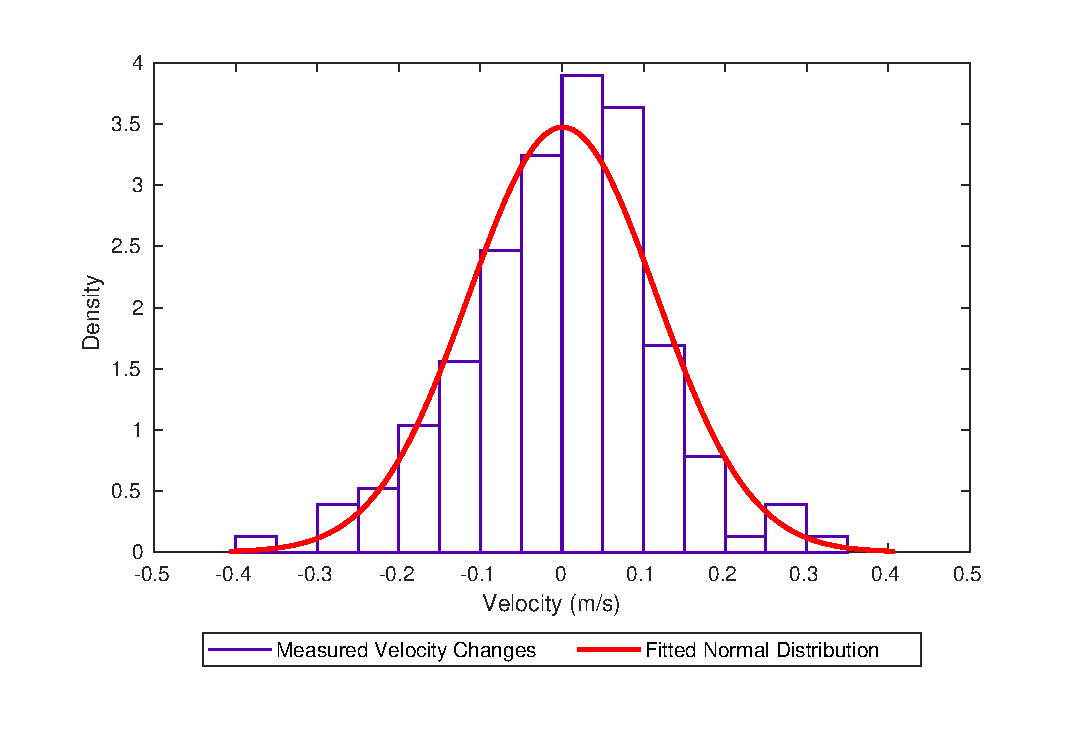
\includegraphics[width=0.8\linewidth]{v_dist.eps}
	\caption{Distribution of measured velocity changes for IU-1 - Pooled Novel \& Base data}\label{fig:v_dist}
\end{figure}

\begin{figure}
	\centering
	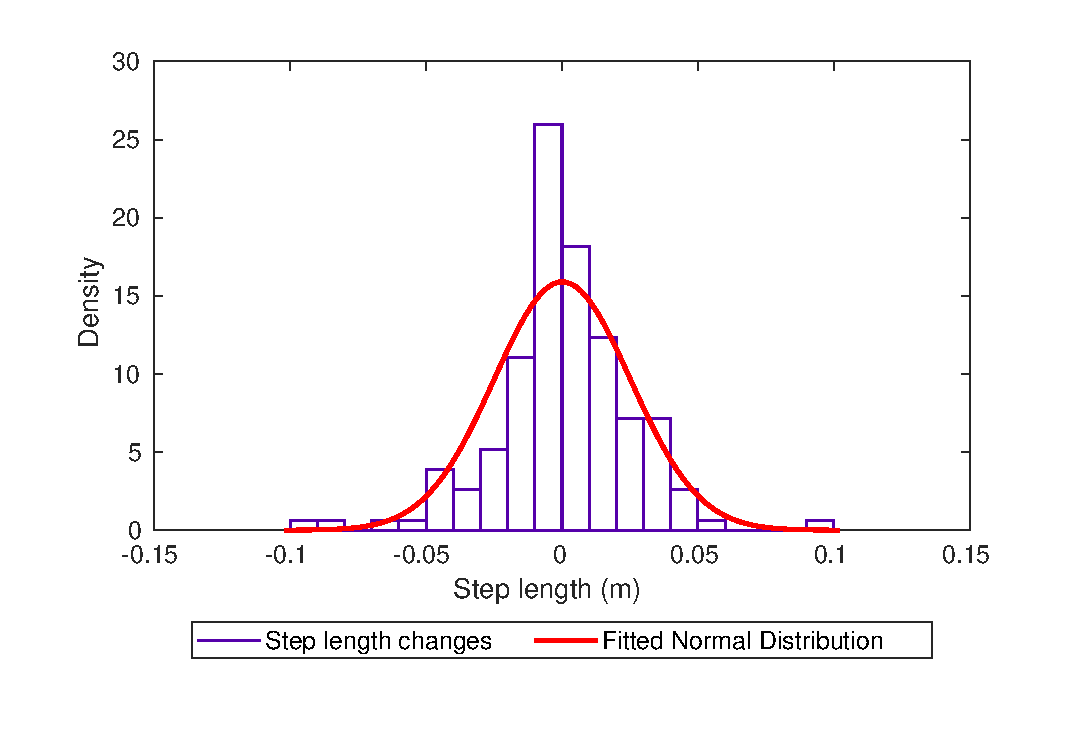
\includegraphics[width=0.8\linewidth]{sl_dist.eps}
	\caption{Distribution of measured step length changes for IU-1 - Pooled Novel \& Base data}\label{fig:sl_dist}
\end{figure}

Approximating gait data with Gaussian distributions motivated transforming the data from healthy user trials to match the mean and standard deviation of  data from an injured user. A transformation was performed on a vector of measurements $ \q_s \in \mathcal{R}^N$ of an individual gait feature,  where $ N $ is the number of  measurements and $ s \in \{ 1 \dots S\}$. A vector containing measurements of a single gait feature is also denoted by $ \q $, with the subscript $ s $ omitted for readability. Its mean and standard deviation are $ \bar{q} $ and $ \sigma $ respectively. Subscripts $ b $ and $ n $ are denote base and novel data respectively and $ n/b $ represents base data that has been transformed to match the distribution of novel data from a single user via:
%
\begin{eqnarray}
	\q_{n/b} &=& (\q_b - \bar{q}_b)\sigma_n \sigma_b^{-1} + \bar{q}_n \label{eq:transform} \\
	\q &\leftarrow& [\q_{n/b}^T\ \q_{n}^T]^T
\end{eqnarray}
The features are then collected in a matrix $ \Q \in \mathcal{R}^{N \times S} $ such that $ \q = [\q_1 \dots \q_S] $. As the objective of this method is to relate changes in gait features to corresponding changes in gait speed, the work that follows considers the changes in gait feature measurements from step-to-step $ \Delta \Q $.

It is important to choose appropriate novel data to ensure that the gait feature data carries a sufficiently high amount of information about the subject's desired gait speed.
\subsubsection{Choosing Appropriate Novel Data}\label{sec:MI}

\begin{figure}
	\centering
	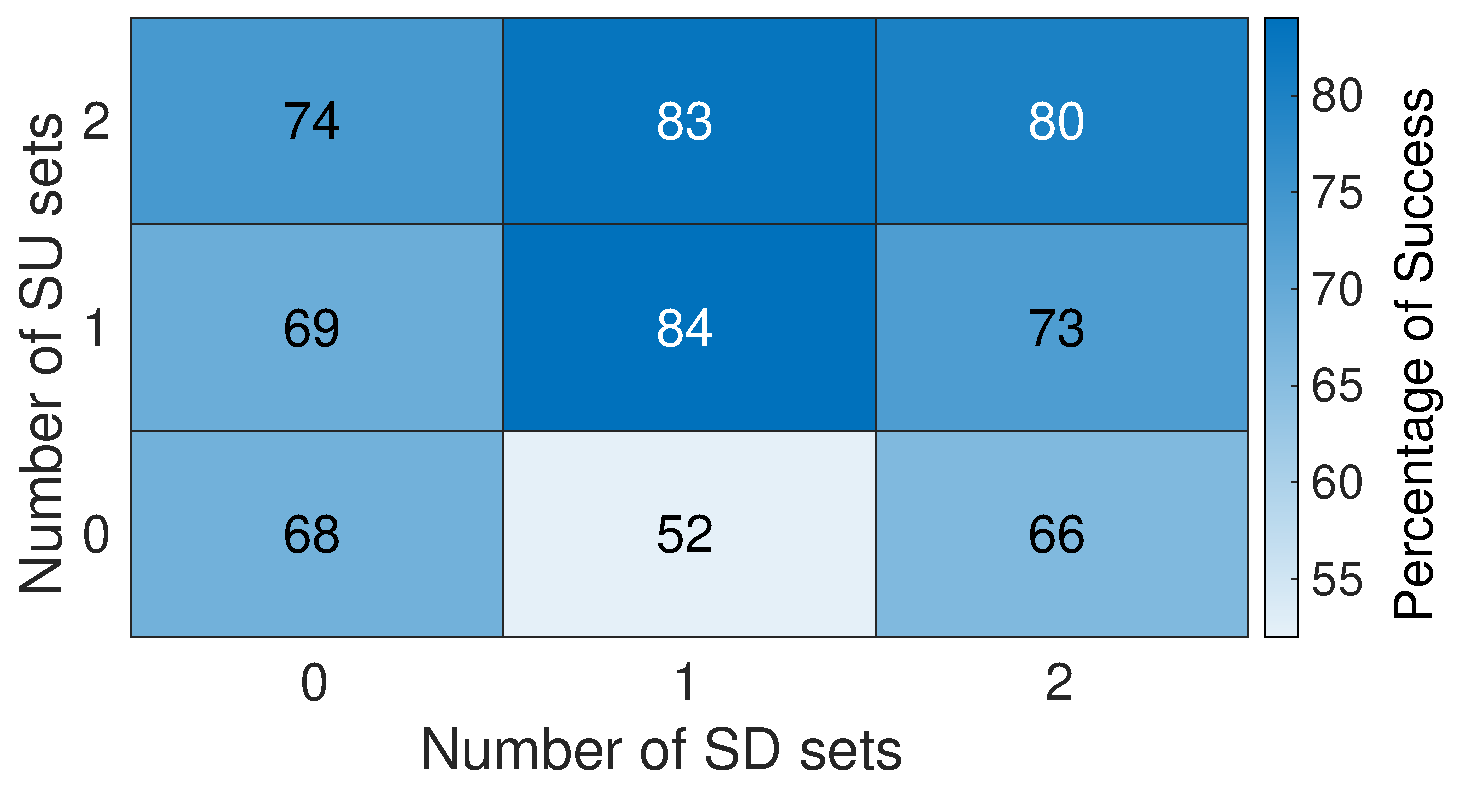
\includegraphics[width=0.65\linewidth]{NAB2_heatmap}
	\caption{Estimator performance for a user with SCI for chosen novel data.}\label{fig:heatmap}
\end{figure}

Steady-state walking in trials of subjects with iSCIs had a standard deviation of up to 0.18 m/s for their walking speed compared to 0.1 m/s seen in healthy users walking without robot assistance \cite{socie2013gait}. In addition to the severity of the iSCI, variability can be affected by user fatigue, discomfort, or misfit orthoses. As a result, some walking trials better represent the exoskeleton user's gait patterns than other trials performed on the same day. Therefore, choosing the appropriate training datasets from injured users is important to reduce noise in the data and accurately capture their gait patterns. Figure~\ref{fig:heatmap} shows the differences in accuracy of different estimator configurations in predicting gait speed changes. Each of these configurations used the same base data but different novel training data from a combination of a number SU/SD trials as listed on the axes. Estimator accuracy differs based on the novel data used for customization, so these data must be chosen carefully. This choice may be increasingly difficult to make as the number of trials to consider increases. 

One way to make this choice is to consider the Mutual Information (MI) between the measured variables (gait features) and those to be inferred (desired speed). MI is a measure of the information obtained about one random variable by observing another variable \cite{cover1999elements}. The MI between two variables may be computed using the Kullback-Leibler (KL) divergence, $ D_{KL} $, between their joint and marginal distributions. For example, consider two distributions $ A $ and $ B $ of an arbitrary variable $ x $. The KL divergence $ D_{KL}(A||B) $ is a measure of how different the two distributions are, as illustrated in Fig.~\ref{fig:divergence}. The mutual information between the two variables $ A $ and $ B $ is $ I(A;B) = D_{KL}(p_{(A,B)}||p_A p_B) $ where $ p_{(A,B)} $ is their joint probability and $ p_A $ and $ p_B $ are their marginal probabilities. Roughly, the MI provides a scalar measure of the correlation between the two variables.
%
\begin{figure}
	\centering
	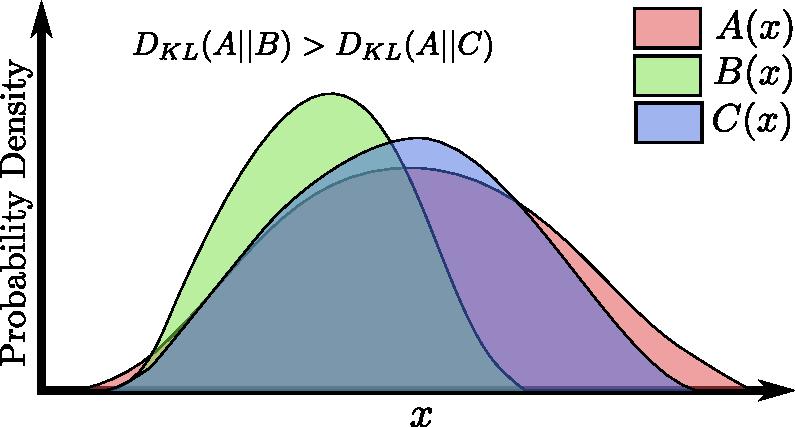
\includegraphics[width=0.6\linewidth]{divergence.pdf}
	\caption{The difference between two distributions may be quantified using KL divergence.}\label{fig:divergence}
\end{figure}

The computation of KL divergence is simplified with the assumption that both distributions are Gaussian. The KL divergence between distributions $ A \sim \mathcal{N}\left(\mmu_a, \Ssigma_a\right) $ and $ B \sim \mathcal{N}\left(\mmu_b, \Ssigma_b\right) $ is given by

\begin{equation}
	D_{KL} (A||B) = \int_{x} P_A(x) \log \frac{P_A(x)}{P_B(x)}dx \label{eq:kl_def}
\end{equation}
%
with the probability density function of a generic multivariate Gaussian random variable $ \x \in \mathbb{R}^k$ with mean $ \mmu \in \mathbb{R}^k $ and covariance $ \Ssigma \in \mathbb{R}^{k \times k}$ given by
%
\[
	p(\x) = \frac{1}{(2\pi)^{k/2} |\Ssigma|^{1/2}} \exp\left(-\frac{1}{2} (\x-\mmu)^T \Ssigma^{-1} (\x-\mmu)\right)
\]
%
%The expected value of a random variable $ X $ is defined as \[\mathbb{E}[X] = \int_{-\infty}^{\infty} x f(x) dx\] therefore, using \eqref{eq:kl_def}, KL divergence may be defined as
%\begin{eqnarray}
%	D_{KL}(A||B) &=&  \mathbb{E}_A \left[\log \frac{A}{B}\right] \nonumber \\
%	{} &=& \mathbb{E}_A \left[\log(A) - \log(B)\right] \label{eq:dkl_exp}
%\end{eqnarray}
%%
Substituting the probability density functions of $ A $ and $ B $ into \eqref{eq:kl_def}, the computation of $ D_{KL}(A||B) $ is simplified \cite{duchi2007derivations} to
%
\begin{equation}
	D_{KL}(A||B) = \frac{1}{2} \left[\log \frac{|\Ssigma_b|}{|\Ssigma_a|} - k + (\mmu_a - \mmu_b)^T \Ssigma_b^{-1} (\mmu_a - \mmu_b) + tr\{\Ssigma_b^{-1} \Ssigma_a\} \right] \label{eq:dkl}
\end{equation}
%
where $ tr\{\Ssigma_b^{-1} \Ssigma_a\} $ is the trace of $\Ssigma_b^{-1} \Ssigma_a $. As $ p_{(A,B)} $ and $ p_A p_B $ have the same dimension, mean, and diagonal of the covariance matrix when computing the MI, the computation of $ I(A;B) $ using \eqref{eq:dkl} further simplifies down to
\begin{equation}
	I(A;B) =\frac{1}{2} \left[\log \frac{|\Ssigma_{ab}^{'}|}{|\Ssigma_{ab}|} \right] \label{eq:MI}
\end{equation}
where $ \Ssigma_{ab} = E[(A - \greekvec{\mu}_a)(B - \greekvec{\mu}_b)^T] $ and $ \Ssigma_{ab}^{'} $ is a block diagonal matrix with the cross-covariance between $ A $ and $ B $ in $ \Ssigma_{ab} $ set to zero. Roughly, the MI provides a scalar measure of the correlation between the two variables.	

MI was used to measure the utility of the measured gait features for estimating the desired gait speed. Since the true desired gait speed is difficult to determine, the speed at the next step, denoted $ v' $, was assumed as its proxy, similar to Chapter~\ref{chapter:BKF}. The distributions of gait speed and features were approximated as Gaussian and the MI $ I(V ; Q) $ was computed, where $ V $ is the distribution of the step-to-step changes in desired speed estimated via $ \Delta v' $, and $ Q $ is the distribution of the corresponding changes in gait feature measurements from step-to-step, estimated from $ \Delta \Q $. The intuition behind using distributions of the changes in gait speed and features is to incorporate the knowledge of their evolution through intent changes into the selection process. 

To avoid training the estimator on all available speed change data and leave some data for testing, the novel training dataset was limited to at most three out of all available trials for each injured user. Combinations of available novel trial data were generated by choosing two or three out of the available number of trials and collected in a set $ W $. The MI was computed for the novel/base data pairing for each combination in the set, stored in a vector $ \greekvec{\iota} \in \mathcal{R}^{{\rm len}(W)}$. The pairing with the highest MI was chosen. Algorithm \ref{algo:selection} details this overall process to select the appropriate novel trial data for augmenting the base data.

\begin{algorithm}
	\caption{Training set selection}\label{algo:selection}
	\begin{algorithmic}[1]
		\Require $ \v'_n$, $\v'_b $, $ \Q_n $, $\Q_b$
		\State {\em Note:} $ W $ denotes a set where each element is a combinations of novel trials to be considered
		\For{$ m = 1 $ to $ {\rm len}(W) $}
		\State $ \v'_{n/b} = (\v'_b - \bar{v}'_b)\sigma_{v'_n} \sigma_{v'_b}^{-1} + \bar{v}'_n $ 
		\State $ \v' \leftarrow [\v_{n/b}^{'T}\ \v_{n}^{'T}]^T $
		\For{$ s = 1 $ to $ S $}
		\State $ \q_{n/b} = (\q_b - \bar{q}_b)\sigma_n \sigma_b^{-1} + \bar{q}_n $ 
		\State $ \q \leftarrow [\q_{n/b}^T\ \q_{n}^T]^T $
		\EndFor
		\State $ \Q = [\q_1 \ \q_2 \dots \q_S] $
		\State $ \v' \leftarrow \Delta \v' $
		\State $ \Q \leftarrow \Delta \Q $
		\vskip 5pt
		\State $ \begin{bmatrix}
			Q \\
			V
		\end{bmatrix} \sim \mathcal{N} \left( \begin{bmatrix}
			\bar{\q} \\
			\bar{v}'
		\end{bmatrix},\begin{bmatrix}
			\Ssigma_{\q \q} & \Ssigma_{\q v'} \\
			\Ssigma_{v' \q} & \Sigma_{v'v'}
		\end{bmatrix}\right) $
		\vskip 2pt
		\State $ \iota_m = I(V;Q) $
		\EndFor
		\State \Return $m$ such that $\iota_m$ = $ \max(\greekvec{\iota}) $ 
	\end{algorithmic}
\end{algorithm}%

\subsection{Estimating the Desired Gait Velocity}\label{sec:models}

Gait features and desired speed were assumed to follow Gaussian distributions during estimation as well. In contrast to Chapter~\ref{chapter:BKF}, let the desired gait speed $ v^d $ be rewritten as $ z $ to simplify notation:
\begin{align}
	\begin{bmatrix}
		\q \\
		z
	\end{bmatrix} &\sim \mathcal{N}\left(\begin{bmatrix}
		\bar{\q} \\
		\bar{z}
	\end{bmatrix},
	\begin{bmatrix}
		\Ssigma_{\q \q} & \Ssigma_{\q z} \\
		\Ssigma_{z \q} & \Sigma_{z z}
	\end{bmatrix}\right) \label{eq:full_dist}
\end{align}
where the means and covariances were computed using the training data that includes both base and novel data. Given measurements $\tilde{\q}$ of the gait features at TD, the estimated mean and variance of the desired gait speed, for the first stage of the BKF, were determined using standard conditional probability equations
\begin{align}
	\hat{z} &= \bar{z} + \Ssigma_{z \q} \Ssigma_{\q \q}^{-1} \left(\tilde{\q} - \bar{\q}\right) \label{eq:v_up} \\	
	\hat{\Sigma}_{z z} &= \Sigma_{z z} - \Ssigma_{z \q} \Ssigma_{\q \q}^{-1} \Ssigma_{\q z} \label{eq:c_up}
\end{align}

The estimate $\hat{z}$ is driven by the error between the training mean $ \bar{\q} $ and gait feature measurements $ \tilde{\q} $. Along with $\hat{z}$, the resulting estimator outputs an SU/SD signal at TD as the difference between $ \hat{z} $ at the current and previous TD. A speed change threshold for a SU/SD was determined by recording the standard deviation in step-to-step speed changes observed from three steady-state walking steps from each trial in the training data. This threshold is important due to the minimal detectable change (MDC) or the minimal change in the measured gait speed required to distinguish between a true change and noise. The MDC for people with iSCIs was shown to be around 0.17~m/s \cite{mohandas2012minimal}.

\section{Results \& Discussion} \label{sec:results}

The performance of data pooling for crutch and walker-assisted walking was evaluated on experimental data (Section~\ref{sec:exoData}) and the efficacy of the algorithm was explored as described in Section~\ref{sec:efficacy}. Initial testing involved using base and novel data from trials using the same ambulatory device, i.e., walker or crutches as presented in Sections~\ref{sec:ww}~and~\ref{sec:cc}. Additional testing was then performed to explore the interchangeability of base data to explore the effects of these ambulatory devices on gait patterns and estimator performance and is described in Section~\ref{sec:interchangeability}.

\subsection{Testing on walking trial data}
One step before and three steps after the speed change command, for a total of four steps, were chosen as training data from all base and novel trials. For each ambulatory device, i.e., crutches or walker, the base data consisted of 6 trials from each uninjured user in each mode, adaptive and free, for a total of 72 trials. While similar user responses to desired speed change exist for free and adaptive mode, they are evident in different sensor measurements, as described in the previous chapter. Despite these differences, more base data was found to result in improved accuracy, even when that data resulted in a mode mismatch between base and novel data. For example, for IU-1, excluding base data from trials in free mode resulted in an estimator accuracy of 69\% compared to 80\% when both free and adaptive mode data were included in the base set. Up to three trials (i.e., 12 steps' worth of data) were selected as novel data for each injured user via Algo.~\ref{algo:selection} and used to transform the base data. The estimator was then run on all available trial data for each subject (38-85 steps) out of which at most 12 steps were seen in training. The estimated change in desired speed was compared to the measured change, and if the speed change sign was correctly anticipated, it was considered a successful estimate.

Figure~\ref{fig:single_trial} visualizes the output of the estimator for an SD trial with IU-1 where the dashed black lines illustrate the speed change threshold used to determine true changes. While the intent signal is represented similarly as in the previous chapter, the accuracy of $ \hat{z} $ was found to be comparatively better due to the revisions to estimator described in this Chapter. Therefore, similarly to Section~\ref{sec:add_analysis}, the RMS error between the predicted gait speed change at TD and the value measured at the subsequent MS was considered while evaluating estimator performance. 

\begin{figure}
	\centering
	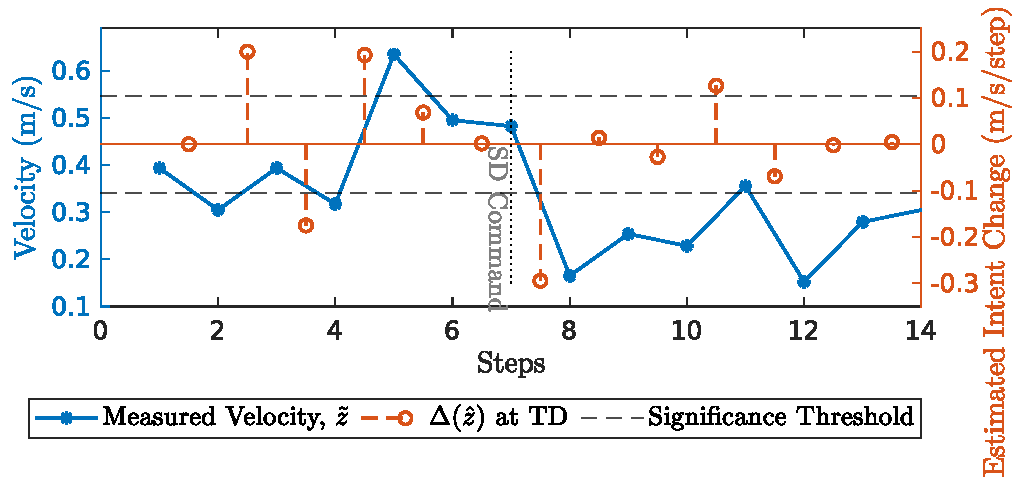
\includegraphics[width=0.9\linewidth]{single_trial.pdf}
	\caption{Output of a single estimator trial for IU-1.}\label{fig:single_trial}
\end{figure}

The  estimator was run in three configurations for both subjects to highlight the benefits of using both novel and base data, as illustrated in Fig.~\ref{fig:novel_comp}. The confusion matrix for the trials of IU-2 is listed in Table~\ref{table:comp_table}. The color of each cell ranges from green to red as the accuracy ranges from 100\% to 0\% therefore, the higher the accuracy, the greener the cell. The base data was from walker trials and the novel data was from walker and crutch trials for IU-1 and IU-2, respectively. The first configuration used untransformed base data (Base\textsubscript{b}), the second used only the transformed base data (Base\textsubscript{n/b}), and the third used both novel and transformed base data (Novel+Base\textsubscript{n/b}). Minor increases in SU/SD identification accuracy were observed (Fig.~\ref{fig:novel_comp}) when using only the transformed base data, as the accuracy depends on identifying only the speed changes, and not their magnitude. Despite increases in accuracy, the RMS errors deteriorated and were unacceptable at 12.8 m/s and 3.6 m/s for IU-1 and IU-2 respectively. Adding novel data to the transformed base data increased the speed change estimation accuracy and decreased the RMS errors. 

\begin{figure}
	\centering
	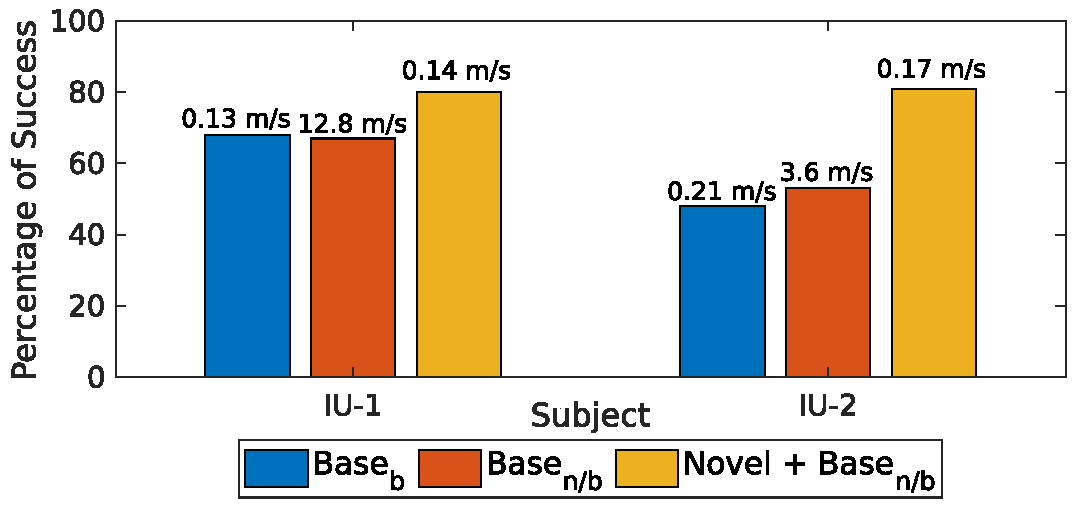
\includegraphics[width=0.8\linewidth]{novel_comp.pdf}
	\caption{Percentage of success with and without novel data for both subjects, labeled with RMS error between predicted and measured gait speed changes.}\label{fig:novel_comp}
\end{figure}

\begin{table}
	\centering
	\caption{Confusion matrix for IU-2 \\ For estimation with and without novel data }\label{table:comp_table}
	\begin{tabular}{|c|c|c|c|c|c|c|}
	\hhline{-------}
	& \multicolumn{3}{c|}{Predicted SD} & \multicolumn{3}{c|}{Predicted SU} \\ 
	\hhline{~------}
	& Base \textsubscript{b} & Base \textsubscript{n/b} & Novel & Base \textsubscript{b} & Base \textsubscript{n/b} & Novel \\
	\hhline{-------}
	Actual SD	& \prescolor{50} & \prescolor{51} & \prescolor{78} & \frescolor{53} & \frescolor{45} & \frescolor{17} \\ %\hhline{---} %6/ & 8/3
	\hline
	Actual SU	&  \frescolor{50} & \frescolor{49} & \frescolor{22} & \prescolor{47}& \prescolor{55} & \prescolor{83} \\ \hhline{-------}%6/ & 7/9
	%			\hline 
\end{tabular}
\end{table}

The trials of IU-1 using only base data had an overall success rate of 68\%. Upon using novel data, the success rate increased to 80\% with a p-value $ p = 0.049$ where the null hypothesis was that the success rate would stay the same. Similarly, the success rate for IU-2 increased from 48\% to 80\% with a p-value $ p = 7\times10^{-5} $. Therefore, using novel data resulted in statistically significant increases in accuracy.

\subsection{Efficacy of the Novel Data Selection Algorithm}\label{sec:efficacy}

The number of possible combinations of novel data in Algo. \ref{algo:selection} for training was 35 for walker trials and 12 for trials with crutches for IU-1. There were fewer trials with walking using crutches, as there was data loss from sensors that hindered the identification of gait events. All combinations of these trials were used as novel data with base data from uninjured subjects using a walker to train conditional models that were used in the estimator. The percentages of success of those estimator trials are shown in Fig.~\ref{fig:rand_box}. The whiskers denote the most extreme points, and the central line denotes the median. The green markers illustrate the success rates observed when the novel data chosen using Algo.~\ref{algo:selection} was used. If novel data is chosen at random, accuracy may be as low as 59\%, however, using the novel data selection algorithm outlined previously ensures a high likelihood of increased success despite not guaranteeing it. The difference between the results shown in green and the maximum success rate shown by the top whisker would be of at most four misclassified steps for both, crutch and walker trials. The increase in accuracy seen in Figure~\ref{fig:novel_comp} after pooling novel and base data further highlights the importance of including user-specific data.

Overall, our analysis showed different outcomes based on the assistive device used in the novel data. This observation motivates the remainder of the analysis herein, which considers the effects of the assistive device on the efficacy of our methods. 

\begin{figure}
	\centering
	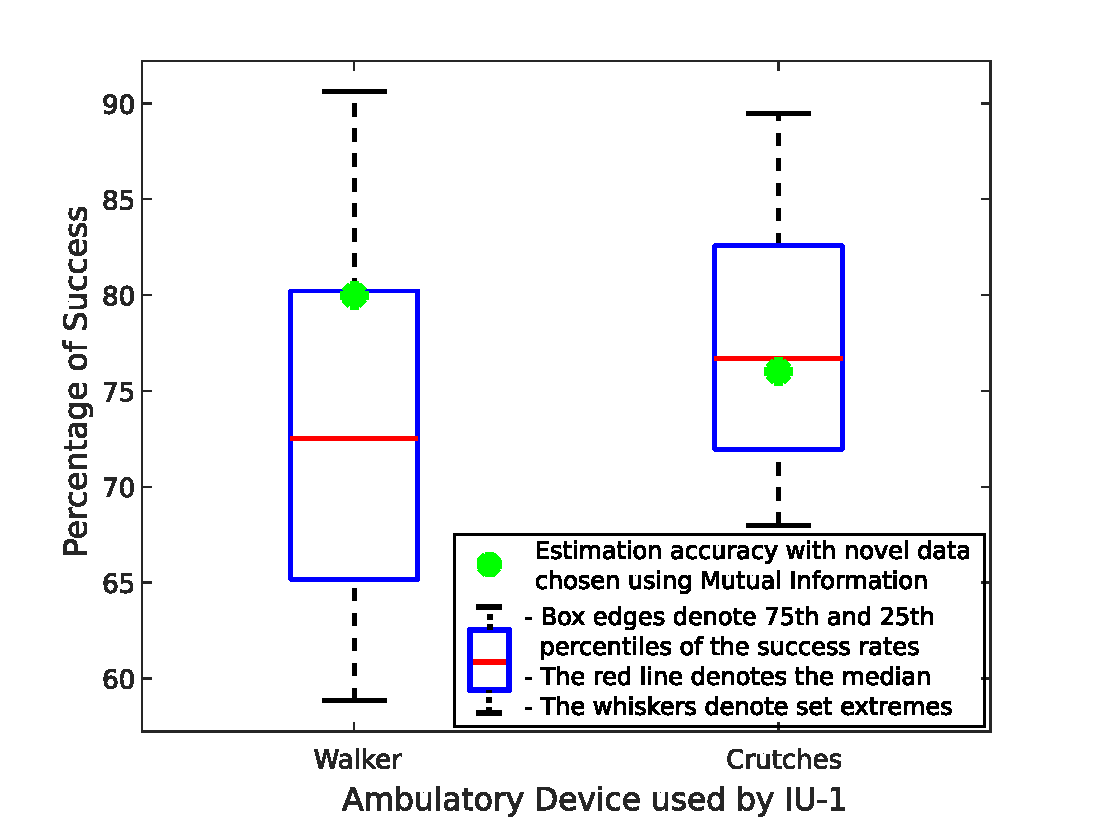
\includegraphics[width=0.86\linewidth]{rand_box_new.pdf}
	\caption{Percentage of success for IU-1 with the base data from walker trials and the novel dataset chosen randomly vs. using Algo. \ref{algo:selection}.}\label{fig:rand_box}
\end{figure}

\subsection{Walking Trials Using Walker}\label{sec:ww}
Estimation for both IU-1 and IU-2 was first performed using base data exclusively from walking trials of uninjured users using walkers. The performance for these users is summarized by the confusion matrix in Table~\ref{table:confmat_w_w}. The estimator for IU-1 was personalized using one SD and two SU trials. The speed change threshold for this estimator configuration was 0.072 m/s, i.e., if the change in predicted speed at TD compared to the measured speed at the previous MS was smaller than this threshold, the SU/SD prediction was ignored. Walking trials for IU-1 had 90 steps, 46 having significant speed changes. 80\% of SU and 81\% of SD changes were accurately detected at TD, for an overall accuracy of 80\% with an RMS speed error of 0.14 m/s.

\begin{table}
	\centering
	\caption{Confusion matrix for \\Novel Data - Walker/Base Data - Walker}\label{table:confmat_w_w}
	\begin{tabular}{|c|c|c|c|c|}
		\hhline{-----}
		& \multicolumn{2}{c|}{Predicted SD} & \multicolumn{2}{c|}{Predicted SU} \\ 
		\hhline{~----}
		& IU-1 & IU-2 & IU-1 & IU-2 \\
		\hhline{-----}
		Actual SD	& \prescolor{80} & \prescolor{58} & \frescolor{19} & \frescolor{78} \\ %\hhline{---} %6/ & 8/3
		\hline
		Actual SU	&  \frescolor{20} & \frescolor{42} & \prescolor{81}& \prescolor{22} \\ \hhline{-----}%6/ & 7/9
		%			\hline 
	\end{tabular}
\end{table}

Similarly for IU-2, the change threshold was 0.13 m/s. Out of the 73 total steps, 21 had significant speed changes, and 58\% SD and 22\% SU changes were accurately detected at TD for an overall accuracy of 43\%. The confusion matrix is given in Table~\ref{table:confmat_w_w}. These trials had higher gait variability as seen from the standard deviation of the steady-state velocity of 0.13 m/s compared to 0.072 m/s for IU-1, which may explain the difficulty in estimation and drop in success rate. Preliminary work suggests other methods to address this low success rate, which are discussed at the end of this section.

\subsection{Walking Trials Using Crutches}\label{sec:cc}

The choice of the assistive device affects gait patterns, so estimation was performed for both injured users for walking trials using crutches with the performance summarized in Table~\ref{table:confmat_c_c}. The base data contained walking trials of uninjured users exclusively using crutches. The speed change threshold was 0.11 m/s. There were 4 significant speed changes in the trials for IU-1, out of which 3 were detected successfully for an overall success rate of 75\% with an RMS error of 1.52 m/s. The success rates of SU and SD are shown in Table~\ref{table:confmat_c_c}.

\begin{table}
	\centering
	\caption{Confusion matrix for \\Novel Data - Crutches/Base Data - Crutches}\label{table:confmat_c_c}
	\begin{tabular}{|c|c|c|c|c|}
		\hhline{-----}
		& \multicolumn{2}{c|}{Predicted SD} & \multicolumn{2}{c|}{Predicted SU} \\ 
		\hhline{~----}
		& IU-1 & IU-2 & IU-1 & IU-2 \\
		\hhline{-----}
		Actual SD	& \prescolor{100} & \prescolor{85} & \frescolor{33} & \frescolor{22} \\ 
		\hline
		Actual SU	&  \frescolor{0} & \frescolor{15} & \prescolor{67}& \prescolor{78} \\ \hhline{-----}
		%			\hline 
	\end{tabular}
\end{table}

The trials for IU-2 had 75 steps, out of which 36 had significant speed changes with a threshold speed of 0.1~m/s. The percentage of success was 81\% with 29 speed changes correctly identified and the rates for SU and SD changes are shown in Table~\ref{table:confmat_c_c}. The RMS error of the speed estimates was 0.2 m/s. A possible explanation for the lower estimator performance for IU-1 is that there may not be enough information about the desired gait speed in the user's gait patterns as evidenced by the amount of MI in the data. The values of MI for the selected novel data for IU-1 and IU-2 were 0.3 and 0.39 respectively. The difference in the $ \iota $ of the two pairings indicates that the gait feature measurements for IU-2 carried roughly 30\% more information about the intended speed than those for IU-1 in this case.

\subsection{Exploring the Interchangeability of Base Data}\label{sec:interchangeability}

Interchangeability of base data was studied to explore the effect of ambulatory devices on estimator accuracy by using different devices for the novel and base data. The first pairing was for IU-1 where the novel data was from trials using crutches and base data was from trials using a walker. The overall success rate for this trial, with 17 significant speed changes, was 76\% and the RMS error was 0.09 m/s. The confusion matrix for this trial is listed in Table~\ref{table:confmat_c_w}. Estimation performed on trial data of IU-2 walking using crutches with base data from trials using a walker yielded a percentage of success of 80\% and an RMS error of 0.17 m/s with the confusion matrix also given in Table~\ref{table:confmat_c_w}. 

\begin{table}
	\centering
	\caption{Confusion matrix for \\Novel Data - Crutches/Base Data - Walker}\label{table:confmat_c_w}
	\begin{tabular}{|c|c|c|c|c|}
		\hhline{-----}
		& \multicolumn{2}{c|}{Predicted SD} & \multicolumn{2}{c|}{Predicted SU} \\ 
		\hhline{~----}
		& IU-1 & IU-2 & IU-1 & IU-2 \\
		\hhline{-----}
		Actual SD	& \prescolor{78} & \prescolor{78} & \frescolor{25} & \frescolor{17} \\ 
		\hline
		Actual SU	&  \frescolor{22} & \frescolor{22} & \prescolor{75}& \prescolor{83} \\ \hhline{-----}
		%			\hline 
	\end{tabular}
\end{table}

These results were compared to estimator trials with IU-1 in which the base data and novel data were both from walking trials with crutches. In this case, the success rate and RMS error were 75\% and 1.52 m/s respectively. Surprisingly, this overall success rate was similar and the RMS error was higher than when the base data was from trials with a walker as in the previous paragraph. Further analysis revealed that the task of gait speed estimation was particularly difficult for IU-1 with crutches since  32 of the 38 steps were below the MDC threshold of 0.17 m/s found in literature. In both of the previous cases, the novel data was the same, only the base data was changed. However, pairing the novel data with walker and crutch base data results in MI values of 0.4048 and 0.3007 respectively, so gait features are more informative of gait speed when uninjured users use a walker. As a result, the model generated using base data from walker trials was able to handle the increased estimation difficulty and increase the estimator accuracy and lower RMS error. This result highlights the flexibility of the estimator to incorporate the most informative base data, even under potentially mismatched conditions.

However, this interchangeability did not hold for every pairing. Estimation was performed for IU-1 with novel data from walking trials with a walker and base data from trials with crutches. Compared to estimation using base data from trials with a walker, the percentage of success dropped to 63\% with an RMS error of 0.12 m/s, and the confusion matrix for this trial is given in Table~\ref{table:confmat_w_c}. There was a less severe deterioration in performance for IU-2. The success rate and RMS error were 38\% and 0.26 m/s, respectively; a difference of 5\% and 0.046 m/s  when  compared to the performance of the same novel data paired with data of trials with a walker (see Section \ref{sec:ww}). 

\begin{table}
	\centering
	\caption{Confusion matrix for \\Novel Data - Walker/Base Data - Crutches}\label{table:confmat_w_c}
	\begin{tabular}{|c|c|c|c|c|}
		\hhline{-----}
		& \multicolumn{2}{c|}{Predicted SD} & \multicolumn{2}{c|}{Predicted SU} \\ 
		\hhline{~----}
		& IU-1 & IU-2 & IU-1 & IU-2 \\
		\hhline{-----}
		Actual SD	& \prescolor{67} & \prescolor{50} & \frescolor{45} & \frescolor{75} \\ 
		\hline
		Actual SU	&  \frescolor{33} & \frescolor{50} & \prescolor{55}& \prescolor{25} \\ \hhline{-----}
		%			\hline 
	\end{tabular}
\end{table}

In general, estimators had higher percentages of success across all tests when using base data of walker trials. This may be as the crutches offer more freedom to move during use than a walker, resulting in more individualized effects on gait patterns across trials. Again, the lower correlation between gait speed and features is evidenced by the MI in the untransformed walker base data (0.3675) being higher than the  crutch base data (0.2813), so gait features are more informative of gait speed when uninjured users use a walker. These inconsistencies could possibly be overcome by adding instrumentation such as IMUs \cite{brescianini2011ins} to crutches to capture their role in gait dynamics. Additionally, upon expanding the base dataset to include both crutch and walker trials, estimator performance either stayed the same or deteriorated. This deterioration is seen when comparing the estimator performance in Tables~\ref{table:confmat_w_w}~and~\ref{table:confmat_w_wc} where the overall accuracy dropped from 80\% to 61\% and the RMS error increased from 0.14 m/s to 0.19 m/s. In the case of IU-2, comparing Tables~\ref{table:confmat_c_c}~and~\ref{table:confmat_c_wc}, the estimator performance is similar with accuracies of 81\% each and RMS errors of 0.17 m/s and 0.16 m/s respectively. These results suggest that choosing subsets of the base data along with novel data (e.g., using extensions of Algo.~\ref{algo:selection}) may allow further improvement in estimator performance.

\begin{table}
	\centering
	\caption{Confusion matrix for \\Novel Data - Walker/Base Data - Walker \& Crutches}\label{table:confmat_w_wc}
	\begin{tabular}{|c|c|c|c|c|}
		\hhline{-----}
		& \multicolumn{2}{c|}{Predicted SD} & \multicolumn{2}{c|}{Predicted SU} \\ 
		\hhline{~----}
		& IU-1 & IU-2 & IU-1 & IU-2 \\
		\hhline{-----}
		Actual SD	& \prescolor{60} & \prescolor{43} & \frescolor{33} & \frescolor{67} \\ 
		\hline
		Actual SU	&  \frescolor{40} & \frescolor{57} & \prescolor{67}& \prescolor{33} \\ \hhline{-----}
		%			\hline 
	\end{tabular}
\end{table}

\begin{table}
	\centering
	\caption{Confusion matrix for \\Novel Data - Crutches/Base Data - Walker \& Crutches}\label{table:confmat_c_wc}
	\begin{tabular}{|c|c|c|c|c|}
		\hhline{-----}
		& \multicolumn{2}{c|}{Predicted SD} & \multicolumn{2}{c|}{Predicted SU} \\ 
		\hhline{~----}
		& IU-1 & IU-2 & IU-1 & IU-2 \\
		\hhline{-----}
		Actual SD	& \prescolor{100} & \prescolor{91} & \frescolor{50} & \frescolor{24} \\ 
		\hline
		Actual SU	&  \frescolor{0} & \frescolor{9} & \prescolor{50}& \prescolor{76} \\ \hhline{-----}
		%			\hline 
	\end{tabular}
\end{table}

Overall, pooling base and novel data improved estimator accuracy in every case except for trials of IU-2 using a walker. This loss of accuracy was due to noisy measurements during those particular trials. The traces of the model covariance matrices when using novel walker and crutch data were 3.425 and 2.015 respectively (for the same base data). Preliminary work shows that this noise in the IU-2 walker data can be attributed to certain noisy features for this user. Multiple gait features often provide the same information about gait speed while introducing unique noise. In such cases, using a reduced, minimally-redundant set of gait features \cite{peng2005feature} offers the potential to further improve accuracy. Preliminary results addressing this aspect show increases of over 20\% in overall estimation accuracy of the IU-2 trials shown in Tables~\ref{table:confmat_w_w}~and~\ref{table:confmat_w_c}. 

For IU-2, estimation was first performed using novel and base data from walker trials. Four minimally redundant features were selected, namely, the step length, the angle and angular velocity of the swing leg, and the angular velocity of the knee of the stance leg. The overall percentage of success increased from 43\%, as seen in Section~\ref{sec:ww}, to 79\% and the RMS error decreased from 0.21 m/s to 0.13 m/s. The confusion matrix for these trials is listed in Table~\ref{table:confmat_wc_red} where the columns show results with different base data pairings. Similarly, when using walker novel data and crutch base data, the only one feature, the time-to-touchdown (tTD), was selected. The overall percentage of success increased from 38\%, as seen in Section~\ref{sec:interchangeability}, to 67\% and the RMS error decreased from 0.26 m/s to 0.19 m/s. 

\begin{table}
	\centering
	\caption{Confusion matrix for IU-2 Walker Trials\\ Using a Reduced Feature Set and Varying Base Data}\label{table:confmat_wc_red}
	\begin{tabular}{|c|c|c|c|c|}
		\hhline{-----}
		& \multicolumn{2}{c|}{Predicted SD} & \multicolumn{2}{c|}{Predicted SU} \\ 
		\hhline{~----}
		& Walker & Crutches & Walker & Crutches \\
		\hhline{-----}
		Actual SD	& \prescolor{80} & \prescolor{83} & \frescolor{25} & \frescolor{50} \\ 
		\hline
		Actual SU	&  \frescolor{20} & \frescolor{17} & \prescolor{75}& \prescolor{50} \\ \hhline{-----}
		%			\hline 
	\end{tabular}
\end{table}

\subsection{Limitations}

The training process assumed that the velocity at the next step was a reliable proxy for the user's desired speed at the current step.  This approach is likely a worse approximation in adaptive mode than in free mode due to the effects of human-robot coupling. However, it may still accurately capture the direction (SU/SD) of the desired speed change, which is the goal of this work.

The number of possible novel/base data pairings makes it difficult to manually choose a pairing to customize the estimator. The presented method automates that choice but it does not provide any guarantee that the selected pairing is the best possible option. This observation is further supported by the study  by Moolchandani et al.,~\cite{moolchandani2021design} where estimation performed with an unoptimized feature set had marginally lower error than when an optimized set was used. 

Data from walking trials of only two subjects with iSCIs were used to evaluate this data selection method. These were experienced users and that experience affects the pHRI during exoskeleton use, as their familiarity with the device may allow them to better predict device behavior and convey their intent more reliably than a novice user. Therefore, it would be beneficial in the future to acquire data from additional trials of both injured and uninjured users with varying degrees of usage proficiency to expand both the novel and base datasets.

Finally, it is noted that the presented results were all obtained in offline evaluation. Assessing methods for integrating the estimated intent into control is an interesting next step, beyond the scope of this dissertation, the details of which will have coupling with the intent signals present for real-time estimation.

\section{Summary} \label{sec:conclusion}
%
This chapter presented a data-driven method for personalized estimation of the intended gait speed of a novel exoskeleton user while addressing the scarcity of training data. Data scarcity is addressed by using a small amount of user-specific data to transform an easily accessible base dataset with data from walking trials of uninjured users. This method relies on commonalities in gait patterns observed across subjects and considers 18 gait features to estimate the user's desire to change speeds. A pairing of novel and base data that well represents the novel user's gait patterns is achieved using the Mutual Information between gait features and gait speed. Conditional Gaussians were used to construct an estimate of the desired speed, which was then used to infer SU/SD changes. In the future, this method may be extended to use the estimated magnitude of the speed change, though additional work may be required to improve the metric quality of the speed estimates. Human limitations on speed change perceptions would set a lower bound of roughly 0.2~m/s for the  accuracy that would be practically noticeable \cite{zhang2015investigation}.
%    \chapter{Personalization of Gait Speed Estimation in the Presence of Data Scarcity}\label{chapter:MP}
	%
	% Conclusion
	\chapter{Summary \& Conclusions}\label{chapter:conc}
\section{Summary}
Inferring user intent is an important step in achieving fluent HRI for robotic exoskeletons. Doing so predictively and intuitively will enable the robot to assist the user in realizing their desired changes while allowing for easy operation of the device. The objective of this dissertation was to develop frameworks to enable such user intent estimation for people with iSCIs using solely the sensors onboard the exoskeleton. In this dissertation, the exoskeleton user's desired gait speed was assumed to represent their intent, as intent is abstract and thus difficult to quantify. The first of the two estimation frameworks presented in this dissertation employs a library containing gaits, generated using the Bipedal Spring Loaded Inverted Pendulum model, that qualitatively emulate human walking. This library is then used to estimate the gait speed and phase of an exoskeleton user via a bank of EKFs running in parallel. The second framework exploits changes in gait patterns of exoskeleton users to infer the corresponding changes in their desired speed. As inter-subject gait variability and the severity of the subjects' injuries present challenges in estimating the user's desire to change speed, a data-driven strategy was presented to customize intent change estimation to fit each subject's individualized gait patterns.

%Estimation of gait speed can be performed using models of human locomotion along with models that correlate changes in gait features and speed. As such, this work draws on concepts from a variety of fields to use these models in appropriate estimation frameworks. %The fundamentals of these concepts are described in Chapter~\ref{chapter:bg_info}. This chapter describes the B-SLIP model of human locomotion, its hybrid dynamics, guard conditions, and reset maps. Poincar\'e surfaces and maps and their application to the B-SLIP model to analyze gait periodicity is also explained. Furthermore, as state estimation is a fundamental component of the objective of this dissertation, an explanation of discrete and extended Kalman Filters is also provided.

Accurate state estimation is necessary for fluent HRI and it can be performed using physics-based models. Human gait patterns can often be accurately described by reduced-order models such as the B-SLIP model. Chapter~\ref{chapter:IMM} described a study of gait patterns observed during slow walking. A linearization-based gait search method was developed to handle the difficulty in optimizing low-speed gaits of the B-SLIP model, which was then used to generate a library of gaits that qualitatively matched human gaits. This library was used in an estimation framework capable of handling the hybrid dynamics of the B-SLIP model. This framework compared sensor measurements from the exoskeleton with library gaits using a bank of parallel Extended Kalman Filters to estimate the most likely gait speed and gait phase. This framework was tested on data from walking trials of an exoskeleton user. It was found that the the accuracy of the estimator depended on how well the library gaits matched human gaits. Therefore, while model-based estimation methods have the potential to easily generalize across individuals, models must be able to accurately emulate human gaits. The insights gained from this work allowed us to anticipate a user's desire to change their intended gait speed.

Foot placement while walking is highly informative of an individual's intended speed as step length varies with gait speed. A two-stage data-driven method to predict a user's desire to speed up or slow down in the future was described in Chapter~\ref{chapter:BKF}. This method leveraged the relationship between user's gait speed and their interactions with the robot and the environment. Using this relationship, a prediction of user's desire to speed up or slow down was made at touchdown before the user realized that change at the next midstance. This predictive nature of this method was in contrast to the reactive nature of many state-of-the-art user intent detection methods, including the framework presented in Chapter~\ref{chapter:IMM}. The estimator was configured to only rely on step length for the trials with the uninjured user and RMS currents of the hip motors were included for the trials with the injured user. The probability of successful intent change inference for the aggregated trials of the uninjured subject was 69\% and that for the user with iSCI was 78\%. The models used in the estimator were trained on all available trial data for the respective user, using up to 78 steps of user-specific data.

The initial formulation of the BKF relied on simple, linear models to establish a relationship between gait speed and gait features such as step length and motor currents. Further analysis, comparing the increase in model complexity versus the number of considered gait features, was performed to increase estimator accuracy. It was found that increasing the number of gait features considered in the estimator resulted in a greater increase in accuracy than increasing model complexity. User trials showed that the physical HRI is user-dependent. This user-dependence was further emphasized upon increasing the number of considered gait features and motivated the personalization of the estimation framework. However, being data-driven, the scarcity of user-specific training data was a challenge in this approach. 

Data scarcity can be addressed by exploiting commonalities in gait patterns that exist across users. Common patterns relating changes in gait speed to changes in gait features, e.g., changes in step length, are observed across exoskeleton users. Easily accessible walking data from healthy exoskeleton can be transformed and pooled with a small amount of novel, user-specific data to increase the available amount of training data while maintaining the user-specificity of the estimator. This pooling can be done with multiple different combinations of trial data and it is difficult to choose the appropriate combination manually. An approach that compared the mutual information between the gait speed and gait feature measurements to choose a combination of novel and base data was described in Chapter~\ref{chapter:MP}. This extended dataset was then used to create models correlating gait features to gait speed to be used in the estimation framework from Chapter~\ref{chapter:BKF}. Data scarcity was addressed as the pooling process only used 8-12 steps' worth of novel user-specific data resulting in a reduction of over 70 steps compared to Chapter~\ref{chapter:BKF}. The average successful estimation of speed-up and slow-down changes increased from 52\% to 67\% with personalization, with a best-case improvement of 32\%, from 48\% to 80\%. 

\section{Future work}

The contributions made in this dissertation have resulted in a variety of directions for future research to advance user intent estimation for lower-limb exoskeletons. A number of potential improvements and extensions are offered below.

\subsection{Refined models for use in the IMM framework}
The work presented in Chapter~\ref{chapter:IMM} shows that the IMM-based framework is dependent on the \com~ trajectories of the library gaits matching those observed in human trials. There are discrepancies between these trajectories that can be reduced through further refinement of the template model. The potential need for modifications to the template is motivated by the additional accuracy required of them in state estimation as compared to previously. The B-SLIP model was historically motivated by the fact that it qualitatively displays the characteristic M-shaped ground reaction force profile of human walking. The use of such models for accurate state estimation requires quantitative accuracy beyond these previous qualitative considerations. Differences in the MI between gait speed and gait features were observed in Chapter~\ref{chapter:MP} due to the effects of assistive devices (walkers or crutches) that were required for use with the exoskeleton. Therefore, one key modification to potentially improve the estimation accuracy would be to address the effects from the assistive device, and incorporate them into the model and the resulting gait library. Another modification to the model would be to use a model that considers torso dynamics. A candidate model may be the B-SLIP with a Virtual Pivot Point (VPP) \cite{maus2010upright}. However, further research to ascertain the applicability of the VPP to the gaits of exoskeleton users is necessary. 

\subsection{Extending the framework to handle other intended actions}

The estimators presented in this dissertation only consider the changes in the user's forward gait speed. However, there are many other actions the user may wish to perform such as gait initiation or termination, turning, i.e., yaw movement, or transitions to/from sitting. In case of the turning motion, for example, the user's desired turn rate and final bearing also need to be estimated. Additional analysis of the available data is required to generate the necessary models to extend the estimation framework and estimate these actions. The lack of hip abduction/adduction in the exoskeleton presents a potential challenge in gathering data for turning actions. Furthermore, the amount of available data related to gait initiation/termination and turning is limited in comparison to forward speed data. This shortage of data motivates the need to conduct further human trials.

\subsection{Extending the dynamics used in the second stage of the BKF}

The second stage of the BKF uses simple dynamics that switch the signs the lateral position and velocity of the CoM to emulate the switching of the stance foot from step-to-step. The simplicity of these dynamics was motivated by the assumption that the motion of the CoM is periodic with respect to the stance foot. Extending these dynamics enabling them to describe non-periodic motion is necessary for the estimator to apply to actions such as turning and gait initiation/termination. Furthermore, the CoM state may also be extended to include the exoskeleton user's bearing.

\subsection{Testing on an increased number of subjects}

The data used to validate the estimators in this dissertation consisted of trials of three uninjured users and two injured users. All of these users were highly experienced exoskeleton users. Their proficiency in the use of the exoskeleton may affect the fluency of their pHRI and subsequently, the performance of the estimator. It may be beneficial to increase the number of subjects to assess the robustness of the estimator and the data augmentation method to inter-subject variability. Additionally, the estimator may also be tested on data from novice users to explore any challenges that may arise from less fluent pHRI as compared to experienced users.

\subsection{Guarantees about the quality of the pooled data and the selection of appropriate base data}

In Chapter~\ref{chapter:MP}, it was observed that appropriate novel data must be used in training the conditional models for the estimator due to gait variability present across trials. This selection served to capture gait patterns accurately while avoiding forming misleading relationships resulting from noisy trials. However, it is difficult to guarantee that the chosen novel data will result in the best possible estimator performance. Refinements to the data pooling framework towards achieving such a guarantee may be made in the future.

It was also found that walker base data led to uniformly better estimator performance over the use of crutch base data, even when the novel data was for user trials with crutches. This result shows that the selection of appropriate base data needs to be considered to ensure optimal estimator performance. The new data selection algorithm suggests future work to address other configuration options of the data pooling and training process. However, leaving the choice of both base and novel datasets free for selection results in a combinatorial challenge. New methods to address this scaling challenge would be needed. Selecting subsets of the gait features could also be assessed to further improve estimator performance.

\subsection{Exoskeleton control based on intent estimation}

This dissertation describes frameworks to estimate the user's intended gait velocity. However, it is necessary perform tests using control based on the output of these frameworks. The inclusion of user intent estimation in exoskeleton control may further affect pHRI. Studying these effects will help in improving the quality of the estimates output by the frameworks and help increase their robustness to gait variability.

\section{Conclusion}
%
%In summary, this dissertation has developed a data-driven framework to intuitively and predictively estimate an exoskeleton user's desire to change their walking speed. The key benefit of this framework is that the estimate of the sign of the desired speed change is made at touchdown, which will allow the exoskeleton to assist the user in realizing their desired change through the remainder of the step. It is difficult to acquire a sufficiently large quantity of user-specific training data from people with iSCIs to generate the models used in the estimator. To address this challenge, this dissertation has also developed a method to address the scarcity of training data required for use in the estimation estimation framework by pooling user-independent base data with user-specific novel data. This method results in a larger training dataset while customizing the estimator to deal with each subject's individualized walking patterns. This expanded dataset also resulted in improvements to the accuracy of the estimator.

As exoskeleton technology advances, fluent HRI is important considering an SCI patient's dependence on the exoskeleton for locomotion. Estimating user intent via intuitive pHRI can contribute toward increasing this fluency. As a result, users may locomote more naturally and reduce the cognitive load associated with using an assistive device resulting in a more comfortable user experience. While many intent estimation strategies have been designed for prostheses users, limited work exists for exoskeleton users. The contributions of this dissertation are intended to advance this field and address the limitation.

This work uses forward gait speed to represent a user's intent, as intent is difficult to quantify. In the future, this estimation framework may be expanded to handle the estimation of the user's desire to perform other actions such as to initiate/terminate the gait, turn, or the user's desired bearing. These developments combined, will allow easier use of the exoskeleton, leading to improved patient outcomes and quality of life.
	
	
	\appendix
	
	% If you have appendices, add them here.
	% Begin each one with \chapter{TITLE} as before. The \appendix command takes
	% care of renaming chapter headings and creates a new page in the Table of
	% Contents for them.
	% \include{appendix-one}
	
	\backmatter              % Place for bibliography and index
	
	
	\bibliographystyle{nddiss2e}
	\bibliography{references.bib}           % input the bib-database file name
	
	
\end{document}

%%
\endinput
%%
%% End of file `template.tex'.
